% Options for packages loaded elsewhere
\PassOptionsToPackage{unicode}{hyperref}
\PassOptionsToPackage{hyphens}{url}
%
\documentclass[
  12pt,
]{article}
\usepackage{amsmath,amssymb}
\usepackage{lmodern}
\usepackage{iftex}
\ifPDFTeX
  \usepackage[T1]{fontenc}
  \usepackage[utf8]{inputenc}
  \usepackage{textcomp} % provide euro and other symbols
\else % if luatex or xetex
  \usepackage{unicode-math}
  \defaultfontfeatures{Scale=MatchLowercase}
  \defaultfontfeatures[\rmfamily]{Ligatures=TeX,Scale=1}
\fi
% Use upquote if available, for straight quotes in verbatim environments
\IfFileExists{upquote.sty}{\usepackage{upquote}}{}
\IfFileExists{microtype.sty}{% use microtype if available
  \usepackage[]{microtype}
  \UseMicrotypeSet[protrusion]{basicmath} % disable protrusion for tt fonts
}{}
\makeatletter
\@ifundefined{KOMAClassName}{% if non-KOMA class
  \IfFileExists{parskip.sty}{%
    \usepackage{parskip}
  }{% else
    \setlength{\parindent}{0pt}
    \setlength{\parskip}{6pt plus 2pt minus 1pt}}
}{% if KOMA class
  \KOMAoptions{parskip=half}}
\makeatother
\usepackage{xcolor}
\IfFileExists{xurl.sty}{\usepackage{xurl}}{} % add URL line breaks if available
\IfFileExists{bookmark.sty}{\usepackage{bookmark}}{\usepackage{hyperref}}
\hypersetup{
  pdftitle={Supplementary Online Content},
  hidelinks,
  pdfcreator={LaTeX via pandoc}}
\urlstyle{same} % disable monospaced font for URLs
\usepackage[margin=1in]{geometry}
\usepackage{graphicx}
\makeatletter
\def\maxwidth{\ifdim\Gin@nat@width>\linewidth\linewidth\else\Gin@nat@width\fi}
\def\maxheight{\ifdim\Gin@nat@height>\textheight\textheight\else\Gin@nat@height\fi}
\makeatother
% Scale images if necessary, so that they will not overflow the page
% margins by default, and it is still possible to overwrite the defaults
% using explicit options in \includegraphics[width, height, ...]{}
\setkeys{Gin}{width=\maxwidth,height=\maxheight,keepaspectratio}
% Set default figure placement to htbp
\makeatletter
\def\fps@figure{htbp}
\makeatother
\setlength{\emergencystretch}{3em} % prevent overfull lines
\providecommand{\tightlist}{%
  \setlength{\itemsep}{0pt}\setlength{\parskip}{0pt}}
\setcounter{secnumdepth}{-\maxdimen} % remove section numbering
\usepackage{titling}
\pretitle{\begin{center}\huge\bfseries}
\posttitle{\end{center}}
\usepackage{pdflscape}
\newcommand{\blandscape}{\begin{landscape}}
\newcommand{\elandscape}{\end{landscape}}
\usepackage{geometry}
\renewcommand\contentsname{Table of Contents}
\usepackage{caption}
\captionsetup[table]{labelformat=empty}
\usepackage{booktabs}
\usepackage{longtable}
\usepackage{array}
\usepackage{multirow}
\usepackage{wrapfig}
\usepackage{float}
\usepackage{colortbl}
\usepackage{pdflscape}
\usepackage{tabu}
\usepackage{threeparttable}
\usepackage{threeparttablex}
\usepackage[normalem]{ulem}
\usepackage{makecell}
\usepackage{xcolor}
\ifLuaTeX
  \usepackage{selnolig}  % disable illegal ligatures
\fi

\title{\textbf{Supplementary Online Content}}
\usepackage{etoolbox}
\makeatletter
\providecommand{\subtitle}[1]{% add subtitle to \maketitle
  \apptocmd{\@title}{\par {\large #1 \par}}{}{}
}
\makeatother
\subtitle{Antithrombotic Regimens for the Prevention of Major Adverse
Cardiac Events in Patients with Chronic Coronary Syndrome - A Systematic
Review and Network Meta-Analysis}
\author{}
\date{\vspace{-2.5em}}

\begin{document}
\maketitle

\newpage 
\tableofcontents 
\newpage

\newpage

\hypertarget{systematic-review}{%
\section{Systematic Review}\label{systematic-review}}

\hypertarget{search-strategies}{%
\subsection{Search Strategies}\label{search-strategies}}

\begingroup\fontsize{9.3}{11.3}\selectfont

\begin{tabu} to \linewidth {>{}l>{\raggedright}X}
\hline
Database & Terms\\
\hline
\cellcolor{gray!6}{\textbf{PubMed}} & \cellcolor{gray!6}{(“Arteriosclerosis”[mh] OR “Angina, Stable”[mh]) AND (“Platelet Aggregation Inhibitors” [Mesh] OR “Dual Anti-Platelet Therapy” [Mesh] OR “Aspirin”[mh] OR “Clopidogrel”[mh] OR “Factor Xa Inhibitors”[mh] OR “apixaban”[Supplementary Concept] OR “edoxaban”[Supplementary Concept] OR “Rivaroxaban”[mh] OR “Purinergic P2Y Receptor Antagonists”[mh] OR “Ticagrelor”[mh] OR “Prasugrel”[tw] OR “Vorapaxar”[tw]) AND (“Myocardial Infarction”[mh] OR “Angina, Unstable”[mh] OR “Stroke”[Mesh] OR Death, Sudden, Cardiac [Mesh] OR “Myocardial Revascularization”[mh] OR “Major Adverse Cardiac Event”[tw] OR “Hemorrhage”[mh])}\\
\hline
\textbf{EMBASE} & (‘atherosclerosis’/exp OR ‘stable angina pectoris’/exp) AND (‘antithrombocytic agent’/exp OR ‘dual antiplatelet therapy’/exp OR ‘acetylsalicylic acid’/mj OR ‘clopidogrel’/mj OR ‘blood clotting factor 10a inhibitor’/exp OR ‘apixaban’/mj OR ‘edoxaban’/mj OR ‘rivaroxaban’/mj OR ‘purinergic p2y receptor antagonist’/exp OR ‘ticagrelor’/mj OR ‘prasugrel’/mj OR ‘vorapaxar’/mj) AND (‘heart infarction’/mj OR ‘unstable angina pectoris’/mj OR ’cerebrovascular accident’/mj OR ‘heart muscle revascularization’/exp OR ‘major adverse cardiac event’/mj OR ‘bleeding’/exp)\\
\hline
CENTRAL & /\#1 MeSH descriptor: [Arteriosclerosis] explode all trees 11018
/\#2 MeSH descriptor: [Angina, Stable] explode all trees 360
/\#3 \#1 OR \#2 11264
/\#4 MeSH descriptor: [Platelet Aggregation Inhibitors] explode all trees 4016
/\#5 MeSH descriptor: [Dual Anti-Platelet Therapy] explode all trees 45
/\#6 MeSH descriptor: [Aspirin] explode all trees 6018
/\#7 MeSH descriptor: [Clopidogrel] explode all trees 2074
/\#8 MeSH descriptor: [Factor Xa Inhibitors] explode all trees 572
/\#9 (apixaban):ti,ab,kw 984
/\#10 (edoxaban):ti,ab,kw 598
/\#11 MeSH descriptor: [Rivaroxaban] explode all trees 568
/\#12 MeSH descriptor: [Purinergic P2Y Receptor Antagonists] explode all trees 359
/\#13 MeSH descriptor: [Ticagrelor] explode all trees 786
/\#14 \#4 OR \#5 OR \#6 OR \#7 OR \#8 OR \#9 OR \#10 OR \#11 OR \#12 OR \#13 10962
/\#15 MeSH descriptor: [Myocardial Infarction] explode all trees 11333
/\#16 MeSH descriptor: [Angina, Unstable] explode all trees 1138
/\#17 MeSH descriptor: [Stroke] explode all trees 10342
/\#18 MeSH descriptor: [Death, Sudden, Cardiac] explode all trees 635
/\#19 MeSH descriptor: [Myocardial Revascularization] explode all trees 9254
/\#20 (Major Adverse Cardiac Event):ti,ab,kw 2745
/\#21 MeSH descriptor: [Hemorrhage] explode all trees 14754
/\#22 \#15 OR \#16 OR \#17 OR \#18 OR \#19 OR \#20 OR \#21 43672
\cellcolor{gray!6}{\textbf{/\#23 \#3 AND \#14 AND \#22}}\\
\hline
\end{tabu}
\endgroup{}

\newpage

\hypertarget{etable-1-trial-definitions}{%
\subsection{eTable 1: Trial
definitions}\label{etable-1-trial-definitions}}

\begingroup\fontsize{9.5}{11.5}\selectfont

\begin{tabu} to \linewidth {>{}l>{\raggedright}X>{\raggedright}X}
\hline
Study & MACE trial definition & Safety endpoint definition\\
\hline
\cellcolor{gray!6}{\textbf{DAPT}} & \cellcolor{gray!6}{Composite of death, myocardial infarction, or stroke during the randomized treatment period month 12 to month 30.} & \cellcolor{gray!6}{Incidence of moderate or severe bleeding during the randomized treatment period month 12 to month 30 assessed according to the Global Utilization of Streptokinase and Tissue Plasminogen Activator for Occluded Arteries [GUSTO] criteria.*}\\
\hline
\textbf{COMPASS} & Composite of cardiovascular death, stroke, or myocardial infarction. & Modification of the International Society on Thrombosis and Haemostasis (ISTH) criteria for major bleeding and included fatal bleeding, symptomatic bleeding into a critical organ, bleeding into a surgical site requiring reoperation, and bleeding that led to hospitalization (including presentation to an acute care facility without an overnight stay). Unlike the ISTH criteria, we considered all bleeding that led to presentation to an acute care facility or hospitalization as major.\\
\hline
\cellcolor{gray!6}{\textbf{HOST-EXAM}} & \cellcolor{gray!6}{Composite of cardiac death, non-fatal myocardial infarction, ischaemic stroke, readmission due to acute coronary syndrome, and definite or probable stent thrombosis (originally referred to as "thrombotic composite outcome").} & \cellcolor{gray!6}{Major bleeding, that  was defined as Bleeding Academic Research Consortium (BARC) type bleeding of least 3.**}\\
\hline
\textbf{THEMIS} & Composite of cardiovascular death, myocardial infarction, or stroke. & TIMI major bleeding. ***\\
\hline
\cellcolor{gray!6}{\textbf{PEGASUS}} & \cellcolor{gray!6}{Composite of cardiovascular death, myocardial infarction, or stroke.} & \cellcolor{gray!6}{Major bleeding, which was defined according to the TIMI classification.***}\\
\hline
\end{tabu}
\endgroup{}

\footnotesize

* Moderate bleeding is defined as bleeding requiring blood transfusion,
but not resulting in hemodynamic compromise, and severe bleeding is
defined as either an intracerebral hemorrhage or bleeding resulting in
substantial hemodynamic compromise requiring treatment according to the
GUSTO criteria.

** BARC type bleeding of 3 is defined as clinical, laboratory, and/or
imaging evidence of bleeding with healthcare responses, as listed: Any
transfusion with overt bleeding; Overt bleeding plus hemoglobin (Hb)
drop \textgreater=3 to \textless5 g/dI (provided Hb drop is related to
bleeding); Overt bleeding plus Hb drop \textgreater=5 g/dl; Cardiac
tamponade; Bleeding requiring surgical intervention for control;
Bleeding requiring intravenous vasoactive drugs; Intracranial
hemorrhage; Intraocular bleed compromising vision.

*** TIMI major bleeding is defined as any intracranial bleeding
(excluding microhemorrhages \textless10 mm evident only on gradient-echo
MRI), or clinically overt signs of hemorrhage associated with a drop in
hemoglobin of \textgreater=5 g/dL or a \textgreater=15\% absolute
decrease in haematocrit, or a fatal bleeding (bleeding that directly
results in death within 7 d).

\normalsize

\hypertarget{efigure-1-effect-modifiers}{%
\subsection{eFigure 1: Effect
Modifiers}\label{efigure-1-effect-modifiers}}

\begin{center}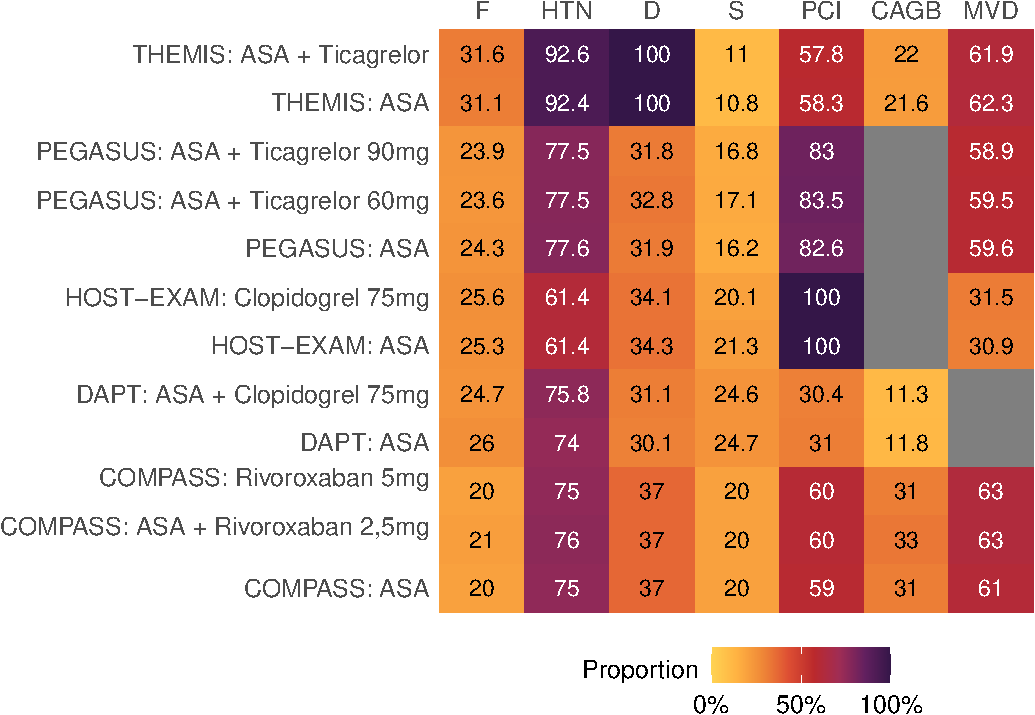
\includegraphics{03_supplementary_files/figure-latex/unnamed-chunk-4-1} \end{center}

Heatmap on the proportions of potential efffect modifiers across
included studies and treatment arms. Each row corresponds to a specific
study and treatment arm combination. Each column corresponds to a
specific effect modifier. The exact proportion is depicted by both
filled color and the number on top in each cell.

Abbreviations: F, female; HTN, hypertension; D, diabetes; S, smoker;
PCI, percutaneous coronary intervention; CAGB, coronary artery bypass
graft; MVD, multivessel disease.

\newpage

\hypertarget{etable-2-risk-of-bias-assessment}{%
\subsection{eTable 2: Risk of Bias
Assessment}\label{etable-2-risk-of-bias-assessment}}

Risk of bias for domain-level as well as overall judgements.

D1: bias arising from randomisation process; D2: bias arising from
deviations from intended interventions; D3: bias due to missing outcome
data; D4: bias in measurement of the outcome; D5: bias in selection of
the reported result.

\hypertarget{mace}{%
\subsubsection{MACE}\label{mace}}

\begin{table}[!h]
\centering
\resizebox{\linewidth}{!}{
\begin{tabular}[t]{lllllll}
\toprule
Study, Comparison & D1 & D2 & D3 & D4 & D5 & Overall\\
\midrule
THEMIS, ASA + Ticagrelor 60mg vs.ASA & \cellcolor[HTML]{5CA881}{\textcolor{white}{Low}} & \cellcolor[HTML]{5CA881}{\textcolor{white}{Low}} & \cellcolor[HTML]{5CA881}{\textcolor{white}{Low}} & \cellcolor[HTML]{5CA881}{\textcolor{white}{Low}} & \cellcolor[HTML]{5CA881}{\textcolor{white}{Low}} & \cellcolor[HTML]{5CA881}{\textcolor{white}{Low}}\\
THEMIS, ASA + Ticagrelor 90mg vs.ASA & \cellcolor[HTML]{5CA881}{\textcolor{white}{Low}} & \cellcolor[HTML]{5CA881}{\textcolor{white}{Low}} & \cellcolor[HTML]{5CA881}{\textcolor{white}{Low}} & \cellcolor[HTML]{5CA881}{\textcolor{white}{Low}} & \cellcolor[HTML]{5CA881}{\textcolor{white}{Low}} & \cellcolor[HTML]{5CA881}{\textcolor{white}{Low}}\\
THEMIS, ASA + Pooled Ticagrelor vs.ASA & \cellcolor[HTML]{5CA881}{\textcolor{white}{Low}} & \cellcolor[HTML]{5CA881}{\textcolor{white}{Low}} & \cellcolor[HTML]{5CA881}{\textcolor{white}{Low}} & \cellcolor[HTML]{5CA881}{\textcolor{white}{Low}} & \cellcolor[HTML]{5CA881}{\textcolor{white}{Low}} & \cellcolor[HTML]{5CA881}{\textcolor{white}{Low}}\\
PEGASUS, ASA + Ticagrelor 60mg vs.ASA & \cellcolor[HTML]{5CA881}{\textcolor{white}{Low}} & \cellcolor[HTML]{5CA881}{\textcolor{white}{Low}} & \cellcolor[HTML]{5CA881}{\textcolor{white}{Low}} & \cellcolor[HTML]{5CA881}{\textcolor{white}{Low}} & \cellcolor[HTML]{5CA881}{\textcolor{white}{Low}} & \cellcolor[HTML]{5CA881}{\textcolor{white}{Low}}\\
PEGASUS, ASA + Ticagrelor 90mg vs.ASA & \cellcolor[HTML]{5CA881}{\textcolor{white}{Low}} & \cellcolor[HTML]{5CA881}{\textcolor{white}{Low}} & \cellcolor[HTML]{5CA881}{\textcolor{white}{Low}} & \cellcolor[HTML]{5CA881}{\textcolor{white}{Low}} & \cellcolor[HTML]{5CA881}{\textcolor{white}{Low}} & \cellcolor[HTML]{5CA881}{\textcolor{white}{Low}}\\
\addlinespace
PEGASUS, ASA + Pooled Ticagrelor vs.ASA & \cellcolor[HTML]{5CA881}{\textcolor{white}{Low}} & \cellcolor[HTML]{5CA881}{\textcolor{white}{Low}} & \cellcolor[HTML]{5CA881}{\textcolor{white}{Low}} & \cellcolor[HTML]{5CA881}{\textcolor{white}{Low}} & \cellcolor[HTML]{5CA881}{\textcolor{white}{Low}} & \cellcolor[HTML]{5CA881}{\textcolor{white}{Low}}\\
DAPT, ASA + Prasugrel 10mg or Clopidogrel 75mg vs.ASA & \cellcolor[HTML]{5CA881}{\textcolor{white}{Low}} & \cellcolor[HTML]{5CA881}{\textcolor{white}{Low}} & \cellcolor[HTML]{5CA881}{\textcolor{white}{Low}} & \cellcolor[HTML]{5CA881}{\textcolor{white}{Low}} & \cellcolor[HTML]{5CA881}{\textcolor{white}{Low}} & \cellcolor[HTML]{5CA881}{\textcolor{white}{Low}}\\
\bottomrule
\end{tabular}}
\end{table}

\hypertarget{bleeding}{%
\subsubsection{Bleeding}\label{bleeding}}

\begin{table}[!h]
\centering
\resizebox{\linewidth}{!}{
\begin{tabular}[t]{lllllll}
\toprule
Study, Comparison & D1 & D2 & D3 & D4 & D5 & Overall\\
\midrule
THEMIS, ASA + Ticagrelor 60mg vs.ASA & \cellcolor[HTML]{5CA881}{\textcolor{white}{Low}} & \cellcolor[HTML]{5CA881}{\textcolor{white}{Low}} & \cellcolor[HTML]{5CA881}{\textcolor{white}{Low}} & \cellcolor[HTML]{5CA881}{\textcolor{white}{Low}} & \cellcolor[HTML]{5CA881}{\textcolor{white}{Low}} & \cellcolor[HTML]{5CA881}{\textcolor{white}{Low}}\\
THEMIS, ASA + Ticagrelor 90mg vs.ASA & \cellcolor[HTML]{5CA881}{\textcolor{white}{Low}} & \cellcolor[HTML]{5CA881}{\textcolor{white}{Low}} & \cellcolor[HTML]{5CA881}{\textcolor{white}{Low}} & \cellcolor[HTML]{5CA881}{\textcolor{white}{Low}} & \cellcolor[HTML]{5CA881}{\textcolor{white}{Low}} & \cellcolor[HTML]{5CA881}{\textcolor{white}{Low}}\\
THEMIS, ASA + Pooled Ticagrelor vs.ASA & \cellcolor[HTML]{5CA881}{\textcolor{white}{Low}} & \cellcolor[HTML]{5CA881}{\textcolor{white}{Low}} & \cellcolor[HTML]{5CA881}{\textcolor{white}{Low}} & \cellcolor[HTML]{5CA881}{\textcolor{white}{Low}} & \cellcolor[HTML]{5CA881}{\textcolor{white}{Low}} & \cellcolor[HTML]{5CA881}{\textcolor{white}{Low}}\\
PEGASUS, ASA + Ticagrelor 60mg vs.ASA & \cellcolor[HTML]{5CA881}{\textcolor{white}{Low}} & \cellcolor[HTML]{5CA881}{\textcolor{white}{Low}} & \cellcolor[HTML]{5CA881}{\textcolor{white}{Low}} & \cellcolor[HTML]{5CA881}{\textcolor{white}{Low}} & \cellcolor[HTML]{5CA881}{\textcolor{white}{Low}} & \cellcolor[HTML]{5CA881}{\textcolor{white}{Low}}\\
PEGASUS, ASA + Ticagrelor 90mg vs.ASA & \cellcolor[HTML]{5CA881}{\textcolor{white}{Low}} & \cellcolor[HTML]{5CA881}{\textcolor{white}{Low}} & \cellcolor[HTML]{5CA881}{\textcolor{white}{Low}} & \cellcolor[HTML]{5CA881}{\textcolor{white}{Low}} & \cellcolor[HTML]{5CA881}{\textcolor{white}{Low}} & \cellcolor[HTML]{5CA881}{\textcolor{white}{Low}}\\
\addlinespace
COMPASS, ASA + Rivaroxaban 2.5mg vs.ASA & \cellcolor[HTML]{5CA881}{\textcolor{white}{Low}} & \cellcolor[HTML]{5CA881}{\textcolor{white}{Low}} & \cellcolor[HTML]{5CA881}{\textcolor{white}{Low}} & \cellcolor[HTML]{5CA881}{\textcolor{white}{Low}} & \cellcolor[HTML]{5CA881}{\textcolor{white}{Low}} & \cellcolor[HTML]{5CA881}{\textcolor{white}{Low}}\\
COMPASS, ASA + Rivaroxaban 2.5mg vs.ASA & \cellcolor[HTML]{5CA881}{\textcolor{white}{Low}} & \cellcolor[HTML]{5CA881}{\textcolor{white}{Low}} & \cellcolor[HTML]{5CA881}{\textcolor{white}{Low}} & \cellcolor[HTML]{E7B03C}{\textcolor{white}{Some concerns}} & \cellcolor[HTML]{5CA881}{\textcolor{white}{Low}} & \cellcolor[HTML]{E7B03C}{\textcolor{white}{Some concerns}}\\
COMPASS, Rivaroxaban 5mg vs.ASA & \cellcolor[HTML]{5CA881}{\textcolor{white}{Low}} & \cellcolor[HTML]{5CA881}{\textcolor{white}{Low}} & \cellcolor[HTML]{5CA881}{\textcolor{white}{Low}} & \cellcolor[HTML]{5CA881}{\textcolor{white}{Low}} & \cellcolor[HTML]{5CA881}{\textcolor{white}{Low}} & \cellcolor[HTML]{5CA881}{\textcolor{white}{Low}}\\
COMPASS, Rivaroxaban 5mg vs.ASA & \cellcolor[HTML]{5CA881}{\textcolor{white}{Low}} & \cellcolor[HTML]{5CA881}{\textcolor{white}{Low}} & \cellcolor[HTML]{5CA881}{\textcolor{white}{Low}} & \cellcolor[HTML]{E7B03C}{\textcolor{white}{Some concerns}} & \cellcolor[HTML]{5CA881}{\textcolor{white}{Low}} & \cellcolor[HTML]{E7B03C}{\textcolor{white}{Some concerns}}\\
HOSTEXAM, Clopidogrel 75mg vs.ASA & \cellcolor[HTML]{5CA881}{\textcolor{white}{Low}} & \cellcolor[HTML]{5CA881}{\textcolor{white}{Low}} & \cellcolor[HTML]{5CA881}{\textcolor{white}{Low}} & \cellcolor[HTML]{5CA881}{\textcolor{white}{Low}} & \cellcolor[HTML]{5CA881}{\textcolor{white}{Low}} & \cellcolor[HTML]{5CA881}{\textcolor{white}{Low}}\\
\addlinespace
DAPT, ASA + Prasugrel 10mg or Clopidogrel 75mg vs.ASA & \cellcolor[HTML]{5CA881}{\textcolor{white}{Low}} & \cellcolor[HTML]{5CA881}{\textcolor{white}{Low}} & \cellcolor[HTML]{5CA881}{\textcolor{white}{Low}} & \cellcolor[HTML]{5CA881}{\textcolor{white}{Low}} & \cellcolor[HTML]{5CA881}{\textcolor{white}{Low}} & \cellcolor[HTML]{5CA881}{\textcolor{white}{Low}}\\
\bottomrule
\end{tabular}}
\end{table}

\newpage

\hypertarget{acute-myocardial-infarction}{%
\subsubsection{Acute Myocardial
Infarction}\label{acute-myocardial-infarction}}

\begin{table}[!h]
\centering
\resizebox{\linewidth}{!}{
\begin{tabular}[t]{lllllll}
\toprule
Study, Comparison & D1 & D2 & D3 & D4 & D5 & Overall\\
\midrule
THEMIS, ASA + Pooled Ticagrelor vs.ASA & \cellcolor[HTML]{5CA881}{\textcolor{white}{Low}} & \cellcolor[HTML]{5CA881}{\textcolor{white}{Low}} & \cellcolor[HTML]{5CA881}{\textcolor{white}{Low}} & \cellcolor[HTML]{5CA881}{\textcolor{white}{Low}} & \cellcolor[HTML]{5CA881}{\textcolor{white}{Low}} & \cellcolor[HTML]{5CA881}{\textcolor{white}{Low}}\\
PEGASUS, ASA + Pooled Ticagrelor vs.ASA & \cellcolor[HTML]{5CA881}{\textcolor{white}{Low}} & \cellcolor[HTML]{5CA881}{\textcolor{white}{Low}} & \cellcolor[HTML]{5CA881}{\textcolor{white}{Low}} & \cellcolor[HTML]{5CA881}{\textcolor{white}{Low}} & \cellcolor[HTML]{5CA881}{\textcolor{white}{Low}} & \cellcolor[HTML]{5CA881}{\textcolor{white}{Low}}\\
COMPASS, ASA + Rivaroxaban 2.5mg vs.ASA & \cellcolor[HTML]{5CA881}{\textcolor{white}{Low}} & \cellcolor[HTML]{5CA881}{\textcolor{white}{Low}} & \cellcolor[HTML]{5CA881}{\textcolor{white}{Low}} & \cellcolor[HTML]{5CA881}{\textcolor{white}{Low}} & \cellcolor[HTML]{5CA881}{\textcolor{white}{Low}} & \cellcolor[HTML]{5CA881}{\textcolor{white}{Low}}\\
COMPASS, Rivaroxaban 5mg vs.ASA & \cellcolor[HTML]{5CA881}{\textcolor{white}{Low}} & \cellcolor[HTML]{5CA881}{\textcolor{white}{Low}} & \cellcolor[HTML]{5CA881}{\textcolor{white}{Low}} & \cellcolor[HTML]{5CA881}{\textcolor{white}{Low}} & \cellcolor[HTML]{5CA881}{\textcolor{white}{Low}} & \cellcolor[HTML]{5CA881}{\textcolor{white}{Low}}\\
HOSTEXAM, Clopidogrel 75mg vs.ASA & \cellcolor[HTML]{5CA881}{\textcolor{white}{Low}} & \cellcolor[HTML]{5CA881}{\textcolor{white}{Low}} & \cellcolor[HTML]{5CA881}{\textcolor{white}{Low}} & \cellcolor[HTML]{5CA881}{\textcolor{white}{Low}} & \cellcolor[HTML]{5CA881}{\textcolor{white}{Low}} & \cellcolor[HTML]{5CA881}{\textcolor{white}{Low}}\\
\addlinespace
DAPT, ASA + Prasugrel 10mg or Clopidogrel 75mg vs.ASA & \cellcolor[HTML]{5CA881}{\textcolor{white}{Low}} & \cellcolor[HTML]{5CA881}{\textcolor{white}{Low}} & \cellcolor[HTML]{5CA881}{\textcolor{white}{Low}} & \cellcolor[HTML]{5CA881}{\textcolor{white}{Low}} & \cellcolor[HTML]{5CA881}{\textcolor{white}{Low}} & \cellcolor[HTML]{5CA881}{\textcolor{white}{Low}}\\
\bottomrule
\end{tabular}}
\end{table}

\hypertarget{ischemic-stroke}{%
\subsubsection{Ischemic Stroke}\label{ischemic-stroke}}

\begin{table}[!h]
\centering
\resizebox{\linewidth}{!}{
\begin{tabular}[t]{lllllll}
\toprule
Study, Comparison & D1 & D2 & D3 & D4 & D5 & Overall\\
\midrule
THEMIS, ASA + Pooled Ticagrelor vs.ASA & \cellcolor[HTML]{5CA881}{\textcolor{white}{Low}} & \cellcolor[HTML]{5CA881}{\textcolor{white}{Low}} & \cellcolor[HTML]{5CA881}{\textcolor{white}{Low}} & \cellcolor[HTML]{5CA881}{\textcolor{white}{Low}} & \cellcolor[HTML]{5CA881}{\textcolor{white}{Low}} & \cellcolor[HTML]{5CA881}{\textcolor{white}{Low}}\\
PEGASUS, ASA + Pooled Ticagrelor vs.ASA & \cellcolor[HTML]{5CA881}{\textcolor{white}{Low}} & \cellcolor[HTML]{5CA881}{\textcolor{white}{Low}} & \cellcolor[HTML]{5CA881}{\textcolor{white}{Low}} & \cellcolor[HTML]{5CA881}{\textcolor{white}{Low}} & \cellcolor[HTML]{5CA881}{\textcolor{white}{Low}} & \cellcolor[HTML]{5CA881}{\textcolor{white}{Low}}\\
COMPASS, ASA + Rivaroxaban 2.5mg vs.ASA & \cellcolor[HTML]{5CA881}{\textcolor{white}{Low}} & \cellcolor[HTML]{5CA881}{\textcolor{white}{Low}} & \cellcolor[HTML]{5CA881}{\textcolor{white}{Low}} & \cellcolor[HTML]{5CA881}{\textcolor{white}{Low}} & \cellcolor[HTML]{5CA881}{\textcolor{white}{Low}} & \cellcolor[HTML]{5CA881}{\textcolor{white}{Low}}\\
COMPASS, Rivaroxaban 5mg vs.ASA & \cellcolor[HTML]{5CA881}{\textcolor{white}{Low}} & \cellcolor[HTML]{5CA881}{\textcolor{white}{Low}} & \cellcolor[HTML]{5CA881}{\textcolor{white}{Low}} & \cellcolor[HTML]{5CA881}{\textcolor{white}{Low}} & \cellcolor[HTML]{5CA881}{\textcolor{white}{Low}} & \cellcolor[HTML]{5CA881}{\textcolor{white}{Low}}\\
HOSTEXAM, Clopidogrel 75mg vs.ASA & \cellcolor[HTML]{5CA881}{\textcolor{white}{Low}} & \cellcolor[HTML]{5CA881}{\textcolor{white}{Low}} & \cellcolor[HTML]{5CA881}{\textcolor{white}{Low}} & \cellcolor[HTML]{5CA881}{\textcolor{white}{Low}} & \cellcolor[HTML]{5CA881}{\textcolor{white}{Low}} & \cellcolor[HTML]{5CA881}{\textcolor{white}{Low}}\\
\addlinespace
DAPT, ASA + Prasugrel 10mg or Clopidogrel 75mg vs.ASA & \cellcolor[HTML]{5CA881}{\textcolor{white}{Low}} & \cellcolor[HTML]{5CA881}{\textcolor{white}{Low}} & \cellcolor[HTML]{5CA881}{\textcolor{white}{Low}} & \cellcolor[HTML]{5CA881}{\textcolor{white}{Low}} & \cellcolor[HTML]{5CA881}{\textcolor{white}{Low}} & \cellcolor[HTML]{5CA881}{\textcolor{white}{Low}}\\
\bottomrule
\end{tabular}}
\end{table}

\hypertarget{all-cause-mortality}{%
\subsubsection{All-cause Mortality}\label{all-cause-mortality}}

\begin{table}[!h]
\centering
\resizebox{\linewidth}{!}{
\begin{tabular}[t]{lllllll}
\toprule
Study, Comparison & D1 & D2 & D3 & D4 & D5 & Overall\\
\midrule
THEMIS, ASA + Pooled Ticagrelor vs.ASA & \cellcolor[HTML]{5CA881}{\textcolor{white}{Low}} & \cellcolor[HTML]{5CA881}{\textcolor{white}{Low}} & \cellcolor[HTML]{5CA881}{\textcolor{white}{Low}} & \cellcolor[HTML]{5CA881}{\textcolor{white}{Low}} & \cellcolor[HTML]{5CA881}{\textcolor{white}{Low}} & \cellcolor[HTML]{5CA881}{\textcolor{white}{Low}}\\
COMPASS, ASA + Rivaroxaban 2.5mg vs.ASA & \cellcolor[HTML]{5CA881}{\textcolor{white}{Low}} & \cellcolor[HTML]{5CA881}{\textcolor{white}{Low}} & \cellcolor[HTML]{5CA881}{\textcolor{white}{Low}} & \cellcolor[HTML]{5CA881}{\textcolor{white}{Low}} & \cellcolor[HTML]{5CA881}{\textcolor{white}{Low}} & \cellcolor[HTML]{5CA881}{\textcolor{white}{Low}}\\
COMPASS, Rivaroxaban 5mg vs.ASA & \cellcolor[HTML]{5CA881}{\textcolor{white}{Low}} & \cellcolor[HTML]{5CA881}{\textcolor{white}{Low}} & \cellcolor[HTML]{5CA881}{\textcolor{white}{Low}} & \cellcolor[HTML]{5CA881}{\textcolor{white}{Low}} & \cellcolor[HTML]{5CA881}{\textcolor{white}{Low}} & \cellcolor[HTML]{5CA881}{\textcolor{white}{Low}}\\
HOSTEXAM, Clopidogrel 75mg vs.ASA & \cellcolor[HTML]{5CA881}{\textcolor{white}{Low}} & \cellcolor[HTML]{5CA881}{\textcolor{white}{Low}} & \cellcolor[HTML]{5CA881}{\textcolor{white}{Low}} & \cellcolor[HTML]{5CA881}{\textcolor{white}{Low}} & \cellcolor[HTML]{5CA881}{\textcolor{white}{Low}} & \cellcolor[HTML]{5CA881}{\textcolor{white}{Low}}\\
DAPT, ASA + Prasugrel 10mg or Clopidogrel 75mg vs.ASA & \cellcolor[HTML]{5CA881}{\textcolor{white}{Low}} & \cellcolor[HTML]{5CA881}{\textcolor{white}{Low}} & \cellcolor[HTML]{5CA881}{\textcolor{white}{Low}} & \cellcolor[HTML]{5CA881}{\textcolor{white}{Low}} & \cellcolor[HTML]{5CA881}{\textcolor{white}{Low}} & \cellcolor[HTML]{5CA881}{\textcolor{white}{Low}}\\
\bottomrule
\end{tabular}}
\end{table}

\hypertarget{cardiovascular-mortality}{%
\subsubsection{Cardiovascular
Mortality}\label{cardiovascular-mortality}}

\begin{table}[!h]
\centering
\resizebox{\linewidth}{!}{
\begin{tabular}[t]{lllllll}
\toprule
Study, Comparison & D1 & D2 & D3 & D4 & D5 & Overall\\
\midrule
THEMIS, ASA + Pooled Ticagrelor vs.ASA & \cellcolor[HTML]{5CA881}{\textcolor{white}{Low}} & \cellcolor[HTML]{5CA881}{\textcolor{white}{Low}} & \cellcolor[HTML]{5CA881}{\textcolor{white}{Low}} & \cellcolor[HTML]{5CA881}{\textcolor{white}{Low}} & \cellcolor[HTML]{5CA881}{\textcolor{white}{Low}} & \cellcolor[HTML]{5CA881}{\textcolor{white}{Low}}\\
PEGASUS, ASA + Pooled Ticagrelor vs.ASA & \cellcolor[HTML]{5CA881}{\textcolor{white}{Low}} & \cellcolor[HTML]{5CA881}{\textcolor{white}{Low}} & \cellcolor[HTML]{5CA881}{\textcolor{white}{Low}} & \cellcolor[HTML]{5CA881}{\textcolor{white}{Low}} & \cellcolor[HTML]{5CA881}{\textcolor{white}{Low}} & \cellcolor[HTML]{5CA881}{\textcolor{white}{Low}}\\
COMPASS, ASA + Rivaroxaban 2.5mg vs.ASA & \cellcolor[HTML]{5CA881}{\textcolor{white}{Low}} & \cellcolor[HTML]{5CA881}{\textcolor{white}{Low}} & \cellcolor[HTML]{5CA881}{\textcolor{white}{Low}} & \cellcolor[HTML]{5CA881}{\textcolor{white}{Low}} & \cellcolor[HTML]{5CA881}{\textcolor{white}{Low}} & \cellcolor[HTML]{5CA881}{\textcolor{white}{Low}}\\
COMPASS, Rivaroxaban 5mg vs.ASA & \cellcolor[HTML]{5CA881}{\textcolor{white}{Low}} & \cellcolor[HTML]{5CA881}{\textcolor{white}{Low}} & \cellcolor[HTML]{5CA881}{\textcolor{white}{Low}} & \cellcolor[HTML]{5CA881}{\textcolor{white}{Low}} & \cellcolor[HTML]{5CA881}{\textcolor{white}{Low}} & \cellcolor[HTML]{5CA881}{\textcolor{white}{Low}}\\
HOSTEXAM, Clopidogrel 75mg vs.ASA & \cellcolor[HTML]{5CA881}{\textcolor{white}{Low}} & \cellcolor[HTML]{5CA881}{\textcolor{white}{Low}} & \cellcolor[HTML]{5CA881}{\textcolor{white}{Low}} & \cellcolor[HTML]{5CA881}{\textcolor{white}{Low}} & \cellcolor[HTML]{5CA881}{\textcolor{white}{Low}} & \cellcolor[HTML]{5CA881}{\textcolor{white}{Low}}\\
\addlinespace
DAPT, ASA + Prasugrel 10mg or Clopidogrel 75mg vs.ASA & \cellcolor[HTML]{5CA881}{\textcolor{white}{Low}} & \cellcolor[HTML]{5CA881}{\textcolor{white}{Low}} & \cellcolor[HTML]{5CA881}{\textcolor{white}{Low}} & \cellcolor[HTML]{5CA881}{\textcolor{white}{Low}} & \cellcolor[HTML]{5CA881}{\textcolor{white}{Low}} & \cellcolor[HTML]{5CA881}{\textcolor{white}{Low}}\\
\bottomrule
\end{tabular}}
\end{table}

\newpage

\begin{landscape}

\hypertarget{pooled-ticagrelor-networks-mace-and-bleeding-outcomes}{%
\section{Pooled Ticagrelor Networks: MACE and Bleeding
Outcomes}\label{pooled-ticagrelor-networks-mace-and-bleeding-outcomes}}

\hypertarget{league-tables}{%
\subsection{League Tables}\label{league-tables}}

\hypertarget{etable-3-median-and-95-credible-intervals}{%
\subsubsection{eTable 3: Median and 95\% Credible
Intervals}\label{etable-3-median-and-95-credible-intervals}}

\begin{table}[!h]
\centering
\resizebox{\linewidth}{!}{
\begin{tabular}[t]{lllllll}
\toprule
  &   &   &   &   &   &  \\
\midrule
ASA & 0.89 (0.78, 1.02) & 0.68 (0.54, 0.88) & 0.74 (0.65, 0.86) & 0.52 (0.39, 0.71) & 0.80 (0.64, 1.00) & 0.87 (0.81, 0.94)\\
1.47 (0.94, 2.21) & Rivaroxaban 5mg & 0.76 (0.57, 1.01) & 0.83 (0.73, 0.96) & 0.59 (0.42, 0.81) & 0.90 (0.70, 1.18) & 0.98 (0.84, 1.14)\\
0.64 (0.42, 0.99) & 0.44 (0.24, 0.77) & Clopidogrel 75mg & 1.09 (0.81, 1.44) & 0.77 (0.52, 1.15) & 1.18 (0.85, 1.66) & 1.28 (0.97, 1.64)\\
1.01 (0.64, 1.61) & 0.69 (0.44, 1.09) & 1.58 (0.85, 2.97) & ASA + Rivaroxaban 2.5mg & 0.71 (0.50, 0.99) & 1.08 (0.83, 1.42) & 1.18 (1.01, 1.38)\\
1.71 (1.02, 2.95) & 1.16 (0.60, 2.34) & 2.67 (1.33, 5.18) & 1.68 (0.84, 3.39) & ASA + Prasugrel 10mg & 1.53 (1.18, 1.97) & 1.67 (1.19, 2.24)\\
\addlinespace
1.53 (1.05, 2.14) & 1.04 (0.58, 1.77) & 2.39 (1.37, 4.22) & 1.50 (0.82, 2.64) & 0.89 (0.60, 1.40) & ASA + Clopidogrel 75mg & 1.09 (0.87, 1.40)\\
2.40 (2.06, 2.83) & 1.63 (1.04, 2.59) & 3.76 (2.42, 6.14) & 2.37 (1.45, 3.85) & 1.41 (0.80, 2.43) & 1.58 (1.07, 2.36) & Pooled Ticagrelor\\
\bottomrule
\end{tabular}}
\end{table}

Hazard ratios (95\% credible interval) for the MACE or Bleeding
outcomes. Treatments are shown in the diagonal. Results to the right of
this diagonal (right upper half table) correspond to the MACE outcome.
Results to the left (left lower half table) correspond to the Bleeding
outcome. Comparisons between treatments should be read from left to
right and the estimate is in the cell in common between the
column-defining treatment and the row-defining treatment. For both
outcomes, a hazard ratio \textless{} 1.0 favors the column-defining
treatment. For example, in the Rivaroxaban 5mg vs.~ASA comparison for
MACE, the corresponding HR (95\% CrI) was 0.89 (0.78, 1.02), favoring
Rivaroxaban 5mg (ie, HR \textless{} 1.0).

\newpage

\hypertarget{etable-4-posterior-probabilities-of-hazard-ratio-1.0}{%
\subsubsection{eTable 4: Posterior Probabilities of Hazard Ratio
\textless{}
1.0}\label{etable-4-posterior-probabilities-of-hazard-ratio-1.0}}

\begin{table}[!h]
\centering
\resizebox{\linewidth}{!}{
\begin{tabular}[t]{lllllll}
\toprule
  &   &   &   &   &   &  \\
\midrule
ASA & 95.31 & 99.88 & 100.00 & 100.00 & 97.26 & 100.00\\
3.92 & Rivaroxaban 5mg & 96.90 & 99.54 & 99.91 & 78.17 & 61.26\\
97.92 & 99.76 & Clopidogrel 75mg & 28.56 & 89.94 & 16.98 & 3.16\\
47.45 & 94.46 & 7.05 & ASA + Rivaroxaban 2.5mg & 97.74 & 27.98 & 2.17\\
2.57 & 33.59 & 0.25 & 7.61 & ASA + Prasugrel 10mg & 0.00 & 0.06\\
\addlinespace
1.03 & 44.61 & 0.05 & 8.58 & 69.67 & ASA + Clopidogrel 75mg & 25.49\\
0.00 & 1.73 & 0.00 & 0.05 & 11.50 & 1.25 & Pooled Ticagrelor\\
\bottomrule
\end{tabular}}
\end{table}

Posterior probabilities (\%) of hazard ratio \textless{} 1.0 for the
MACE or Bleeding outcomes. Treatments are shown in the diagonal. Results
to the right of this diagonal (right upper half table) correspond to the
MACE outcome. Results to the left (left lower half table) correspond to
the Bleeding outcome. Comparisons between treatments should be read from
left to right and the estimate is in the cell in common between the
column-defining treatment and the row-defining treatment. For both
outcomes, a hazard ratio \textless{} 1.0 favors the column-defining
treatment. For example, in the Rivaroxaban 5mg vs.~ASA comparison for
MACE, there was a posterior probability of 95.31\% that the hazard ratio
is below 1.0 (ie, there was a 95.31\% probability for Rivaroxaban 5mg
superiority).

\newpage

\hypertarget{etable-5-posterior-probabilities-of-hazard-ratio-0.8}{%
\subsubsection{eTable 5: Posterior Probabilities of Hazard Ratio
\textless{}
0.8}\label{etable-5-posterior-probabilities-of-hazard-ratio-0.8}}

\begin{table}[!h]
\centering
\resizebox{\linewidth}{!}{
\begin{tabular}[t]{lllllll}
\toprule
  &   &   &   &   &   &  \\
\midrule
ASA & 5.58 & 89.61 & 85.65 & 99.66 & 48.62 & 1.16\\
0.35 & Rivaroxaban 5mg & 62.45 & 29.80 & 96.12 & 18.44 & 0.56\\
85.04 & 97.92 & Clopidogrel 75mg & 1.82 & 57.90 & 1.14 & 0.01\\
15.74 & 73.61 & 1.47 & ASA + Rivaroxaban 2.5mg & 75.70 & 1.14 & 0.00\\
0.24 & 14.39 & 0.04 & 2.01 & ASA + Prasugrel 10mg & 0.00 & 0.00\\
\addlinespace
0.05 & 18.09 & 0.00 & 1.71 & 29.99 & ASA + Clopidogrel 75mg & 0.64\\
0.00 & 0.06 & 0.00 & 0.00 & 2.23 & 0.05 & Pooled Ticagrelor\\
\bottomrule
\end{tabular}}
\end{table}

Posterior probabilities (\%) of hazard ratio \textless{} 0.8 for the
MACE or Bleeding outcomes. Treatments are shown in the diagonal. Results
to the right of this diagonal (right upper half table) correspond to the
MACE outcome. Results to the left (left lower half table) correspond to
the Bleeding outcome. Comparisons between treatments should be read from
left to right and the estimate is in the cell in common between the
column-defining treatment and the row-defining treatment. For both
outcomes, a hazard ratio \textless{} 1.0 favors the column-defining
treatment. For example, in the Rivaroxaban 5mg vs.~ASA comparison for
MACE, there was a posterior probability of 5.58\% that the hazard ratio
is below 0.8 (ie, there was a 5.58\% probability for Rivaroxaban 5mg
superiority).

\newpage

\hypertarget{etable-6-posterior-probabilities-of-hazard-ratio-1.25}{%
\subsubsection{eTable 6: Posterior Probabilities of Hazard Ratio
\textgreater{}
1.25}\label{etable-6-posterior-probabilities-of-hazard-ratio-1.25}}

\begin{table}[!h]
\centering
\resizebox{\linewidth}{!}{
\begin{tabular}[t]{lllllll}
\toprule
  &   &   &   &   &   &  \\
\midrule
ASA & 0.00 & 0.00 & 0.00 & 0.00 & 0.01 & 0.00\\
76.95 & Rivaroxaban 5mg & 0.03 & 0.00 & 0.00 & 0.57 & 0.07\\
0.05 & 0.00 & Clopidogrel 75mg & 17.11 & 0.94 & 36.49 & 57.04\\
18.64 & 0.59 & 76.92 & ASA + Rivaroxaban 2.5mg & 0.05 & 14.91 & 22.07\\
87.24 & 41.85 & 98.52 & 79.15 & ASA + Prasugrel 10mg & 93.88 & 95.88\\
\addlinespace
86.21 & 25.57 & 98.76 & 72.86 & 6.39 & ASA + Clopidogrel 75mg & 12.20\\
100.00 & 87.86 & 100.00 & 99.36 & 66.38 & 87.86 & Pooled Ticagrelor\\
\bottomrule
\end{tabular}}
\end{table}

Posterior probabilities (\%) of hazard ratio \textgreater{} 1.25 for the
MACE or Bleeding outcomes. Treatments are shown in the diagonal. Results
to the right of this diagonal (right upper half table) correspond to the
MACE outcome. Results to the left (left lower half table) correspond to
the Bleeding outcome. Comparisons between treatments should be read from
left to right and the estimate is in the cell in common between the
column-defining treatment and the row-defining treatment. For both
outcomes, a hazard ratio \textless{} 1.0 favors the column-defining
treatment. For example, in the Rivaroxaban 5mg vs.~ASA comparison for
MACE, there was a posterior probability of 0.00\% that the hazard ratio
is above 1.25.

\newpage

\hypertarget{etable-7-posterior-probabilities-of-hazard-ratio-within-the-rope}{%
\subsubsection{eTable 7: Posterior Probabilities of Hazard Ratio within
the
ROPE}\label{etable-7-posterior-probabilities-of-hazard-ratio-within-the-rope}}

\begin{table}[!h]
\centering
\resizebox{\linewidth}{!}{
\begin{tabular}[t]{lllllll}
\toprule
  &   &   &   &   &   &  \\
\midrule
ASA & 94.42 & 10.39 & 14.35 & 0.34 & 51.36 & 98.84\\
22.70 & Rivaroxaban 5mg & 37.52 & 70.20 & 3.88 & 80.99 & 99.36\\
14.91 & 2.08 & Clopidogrel 75mg & 81.06 & 41.16 & 62.38 & 42.95\\
65.62 & 25.80 & 21.60 & ASA + Rivaroxaban 2.5mg & 24.25 & 83.95 & 77.92\\
12.53 & 43.76 & 1.44 & 18.84 & ASA + Prasugrel 10mg & 6.12 & 4.12\\
\addlinespace
13.74 & 56.34 & 1.24 & 25.42 & 63.62 & ASA + Clopidogrel 75mg & 87.16\\
0.00 & 12.07 & 0.00 & 0.64 & 31.40 & 12.09 & Pooled Ticagrelor\\
\bottomrule
\end{tabular}}
\end{table}

Posterior probabilities (\%) of hazard ratio within the region of
practical equivalence (ROPE), ie, between 0.80 and 1.25, for the MACE or
Bleeding outcomes. Treatments are shown in the diagonal. Results to the
right of this diagonal (right upper half table) correspond to the MACE
outcome. Results to the left (left lower half table) correspond to the
Bleeding outcome. Comparisons between treatments should be read from
left to right and the estimate is in the cell in common between the
column-defining treatment and the row-defining treatment. For both
outcomes, a hazard ratio \textless{} 1.0 favors the column-defining
treatment. For example, in the Rivaroxaban 5mg vs.~ASA comparison for
MACE, there was a posterior probability of 94.42\% that the hazard ratio
is within the ROPE.

\end{landscape}

\hypertarget{efigure-2-ranks-with-uncertainty}{%
\subsection{eFigure 2: Ranks with
Uncertainty}\label{efigure-2-ranks-with-uncertainty}}

\begin{center}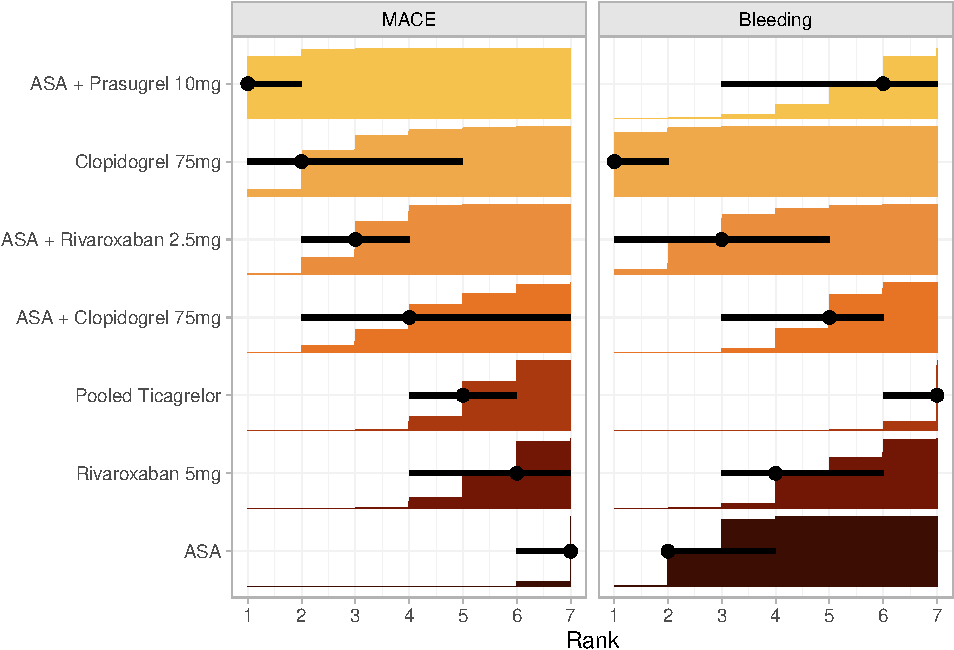
\includegraphics{03_supplementary_files/figure-latex/unnamed-chunk-17-1} \end{center}

Marginal posterior distributions for the rank of each treatment. Left
panel depicts ranks for MACE, while right panel for the Bleeding
outcome. In each panel, there are a point estimate, interval bar, and
bar plot for each treatment (Y-axis). The point estimate represents the
median rank. The interval bar shows the 95\% credible (quantile)
interval of the underlying marginal posterior distribution. Lastly, the
bar plot shows the cumulative distribution function (CDF).

\hypertarget{separate-dosages-ticagrelor-networks-mace-and-bleeding-outcomes}{%
\section{Separate Dosages Ticagrelor Networks: MACE and Bleeding
Outcomes}\label{separate-dosages-ticagrelor-networks-mace-and-bleeding-outcomes}}

\hypertarget{efigure-3-network-plot}{%
\subsection{eFigure 3: Network Plot}\label{efigure-3-network-plot}}

\begin{center}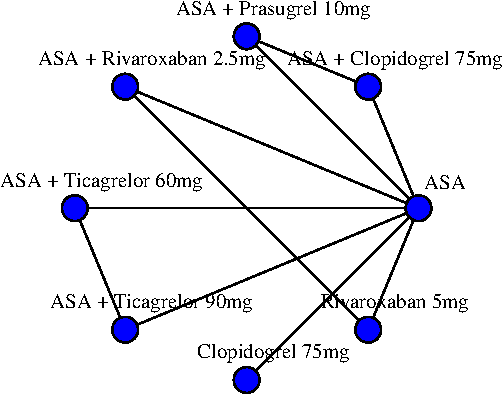
\includegraphics{03_supplementary_files/figure-latex/unnamed-chunk-20-1} \end{center}

\begin{landscape}

\hypertarget{efigure-4-forest-plot}{%
\subsection{eFigure 4: Forest Plot}\label{efigure-4-forest-plot}}

\begin{center}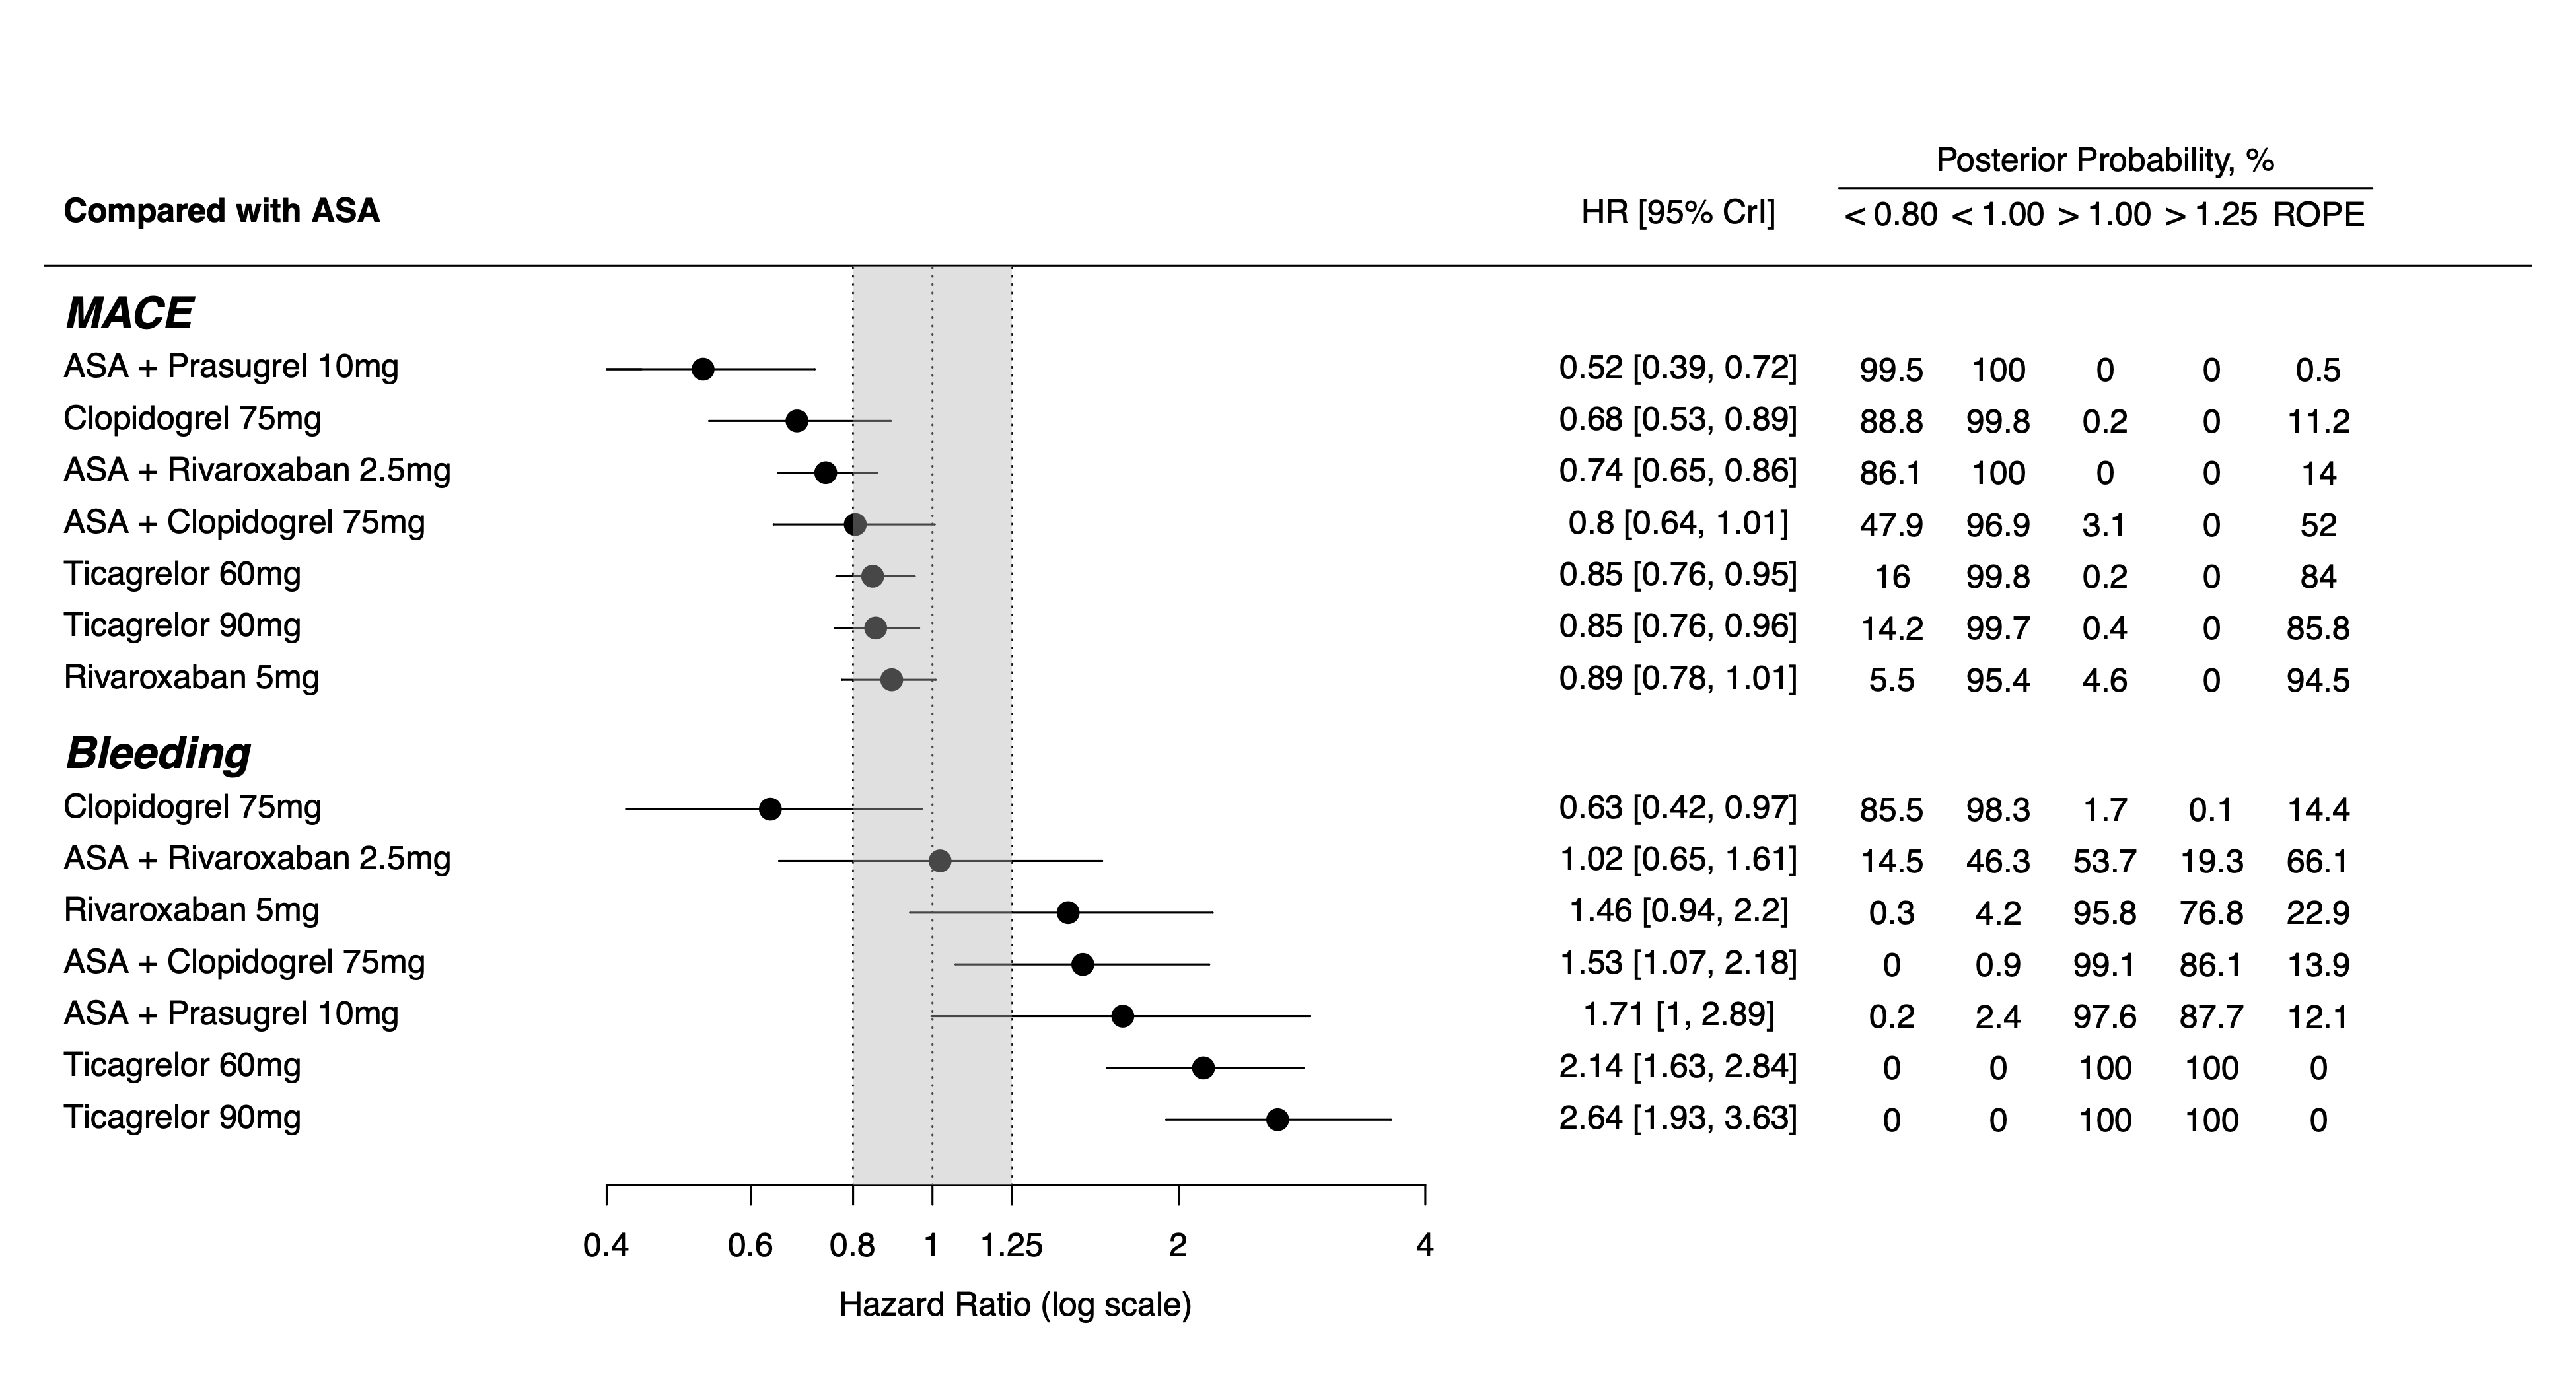
\includegraphics[width=1\linewidth]{/Users/arthur/Coding/projects/active/ARICOCAD_nma/output/plots/supplementary/forest_not_pooled_primary} \end{center}

Left panel: Network of MACE and Bleeding outcomes while separing
Ticagrelor's dosages. Right panel: Treatment effects compared to ASA on
MACE and Bleeding outcomes, ordered according to underlying SUCRA
values. HR below 1.0 favors the experimental treatment. On the left,
treatment names are depicted. In the middle, forest plot shows each
treatment effect median and 95\% credible intervals. Gray area
corresponds to the ROPE (from 0.8 to 1.25 HR). On the right, exact
effect sizes along with posterior probabilities are shown.
Abbreviations: ROPE, region of practical equivalence; HR, hazard ratio.

\hypertarget{league-tables-1}{%
\subsection{League Tables}\label{league-tables-1}}

\hypertarget{etable-8-median-and-95-credible-intervals}{%
\subsubsection{eTable 8: Median and 95\% Credible
Intervals}\label{etable-8-median-and-95-credible-intervals}}

\begin{table}[!h]
\centering
\resizebox{\linewidth}{!}{
\begin{tabular}[t]{llllllll}
\toprule
  &   &   &   &   &   &   &  \\
\midrule
ASA & 0.89 (0.78, 1.01) & 0.85 (0.76, 0.95) & 0.68 (0.53, 0.89) & 0.85 (0.76, 0.96) & 0.74 (0.65, 0.86) & 0.52 (0.39, 0.72) & 0.80 (0.64, 1.01)\\
1.46 (0.94, 2.20) & Rivaroxaban 5mg & 0.95 (0.80, 1.14) & 0.77 (0.58, 1.02) & 0.96 (0.79, 1.14) & 0.83 (0.72, 0.95) & 0.59 (0.42, 0.83) & 0.90 (0.69, 1.17)\\
2.14 (1.63, 2.84) & 1.46 (0.88, 2.46) & Ticagrelor 60mg & 0.81 (0.61, 1.07) & 1.01 (0.90, 1.14) & 0.88 (0.73, 1.04) & 0.62 (0.45, 0.87) & 0.95 (0.74, 1.22)\\
0.63 (0.42, 0.97) & 0.43 (0.24, 0.80) & 0.30 (0.18, 0.49) & Clopidogrel 75mg & 1.25 (0.94, 1.66) & 1.09 (0.81, 1.45) & 0.77 (0.52, 1.16) & 1.18 (0.83, 1.65)\\
2.64 (1.93, 3.63) & 1.80 (1.07, 3.14) & 1.23 (0.83, 1.86) & 4.17 (2.46, 6.83) & Ticagrelor 90mg & 0.87 (0.72, 1.04) & 0.61 (0.45, 0.88) & 0.94 (0.73, 1.23)\\
\addlinespace
1.02 (0.65, 1.61) & 0.70 (0.38, 1.28) & 0.48 (0.28, 0.81) & 1.61 (0.87, 2.97) & 0.39 (0.23, 0.68) & ASA + Rivaroxaban 2.5mg & 0.71 (0.51, 1.01) & 1.08 (0.84, 1.42)\\
1.71 (1.00, 2.89) & 1.17 (0.60, 2.28) & 0.80 (0.44, 1.43) & 2.68 (1.40, 5.31) & 0.64 (0.35, 1.22) & 1.68 (0.86, 3.35) & ASA + Prasugrel 10mg & 1.54 (1.18, 1.97)\\
1.53 (1.07, 2.18) & 1.04 (0.57, 1.74) & 0.71 (0.45, 1.10) & 2.41 (1.33, 4.10) & 0.58 (0.37, 0.93) & 1.50 (0.84, 2.66) & 0.90 (0.51, 1.61) & ASA + Clopidogrel 75mg\\
\bottomrule
\end{tabular}}
\end{table}

Hazard ratios (95\% credible interval) for the MACE or Bleeding
outcomes. Treatments are shown in the diagonal. Results to the right of
this diagonal (right upper half table) correspond to the MACE outcome.
Results to the left (left lower half table) correspond to the Bleeding
outcome. Comparisons between treatments should be read from left to
right and the estimate is in the cell in common between the
column-defining treatment and the row-defining treatment. For both
outcomes, a hazard ratio \textless{} 1.0 favors the column-defining
treatment. For example, in the Rivaroxaban 5mg vs.~ASA comparison for
MACE, the corresponding HR (95\% CrI) was 0.89 (0.78, 1.01), favoring
Rivaroxaban 5mg (ie, HR \textless{} 1.0).

\newpage

\hypertarget{etable-9-posterior-probabilities-of-hazard-ratio-1.0}{%
\subsubsection{eTable 9: Posterior Probabilities of Hazard Ratio
\textless{}
1.0}\label{etable-9-posterior-probabilities-of-hazard-ratio-1.0}}

\begin{table}[!h]
\centering
\resizebox{\linewidth}{!}{
\begin{tabular}[t]{llllllll}
\toprule
  &   &   &   &   &   &   &  \\
\midrule
ASA & 95.41 & 99.83 & 99.80 & 99.65 & 100.00 & 100.00 & 96.94\\
4.19 & Rivaroxaban 5mg & 72.45 & 96.55 & 68.62 & 99.60 & 99.81 & 77.71\\
0.00 & 7.22 & Ticagrelor 60mg & 93.51 & 44.66 & 92.74 & 99.75 & 65.62\\
98.30 & 99.67 & 100.00 & Clopidogrel 75mg & 6.05 & 29.04 & 89.31 & 17.41\\
0.00 & 1.74 & 15.07 & 0.00 & Ticagrelor 90mg & 93.29 & 99.72 & 67.73\\
\addlinespace
46.27 & 87.56 & 99.69 & 6.48 & 99.95 & ASA + Rivaroxaban 2.5mg & 97.45 & 27.45\\
2.43 & 32.60 & 76.79 & 0.10 & 91.61 & 7.49 & ASA + Prasugrel 10mg & 0.04\\
0.86 & 44.02 & 92.47 & 0.09 & 98.98 & 8.45 & 64.12 & ASA + Clopidogrel 75mg\\
\bottomrule
\end{tabular}}
\end{table}

Hazard ratios (95\% credible interval) for the MACE or Bleeding
outcomes. Treatments are shown in the diagonal. Results to the right of
this diagonal (right upper half table) correspond to the MACE outcome.
Results to the left (left lower half table) correspond to the Bleeding
outcome. Comparisons between treatments should be read from left to
right and the estimate is in the cell in common between the
column-defining treatment and the row-defining treatment. For both
outcomes, a hazard ratio \textless{} 1.0 favors the column-defining
treatment. For example, in the Rivaroxaban 5mg vs.~ASA comparison for
MACE, the corresponding HR (95\% CrI) was 95.41, favoring Rivaroxaban
5mg (ie, HR \textless{} 1.0).

\newpage

\hypertarget{etable-10-posterior-probabilities-of-hazard-ratio-0.8}{%
\subsubsection{eTable 10: Posterior Probabilities of Hazard Ratio
\textless{}
0.8}\label{etable-10-posterior-probabilities-of-hazard-ratio-0.8}}

\begin{table}[!h]
\centering
\resizebox{\linewidth}{!}{
\begin{tabular}[t]{llllllll}
\toprule
  &   &   &   &   &   &   &  \\
\midrule
ASA & 5.53 & 16.05 & 88.83 & 14.24 & 86.05 & 99.50 & 47.95\\
0.27 & Rivaroxaban 5mg & 2.69 & 61.99 & 2.41 & 28.99 & 96.06 & 18.36\\
0.00 & 1.16 & Ticagrelor 60mg & 47.15 & 0.00 & 15.75 & 93.44 & 8.50\\
85.49 & 97.67 & 100.00 & Clopidogrel 75mg & 0.11 & 1.98 & 56.94 & 1.32\\
0.00 & 0.14 & 1.93 & 0.00 & Ticagrelor 90mg & 19.01 & 94.04 & 9.84\\
\addlinespace
14.54 & 67.14 & 97.06 & 1.30 & 99.52 & ASA + Rivaroxaban 2.5mg & 75.20 & 1.12\\
0.22 & 13.63 & 50.51 & 0.04 & 74.86 & 1.79 & ASA + Prasugrel 10mg & 0.00\\
0.00 & 17.41 & 68.16 & 0.01 & 90.64 & 1.70 & 35.40 & ASA + Clopidogrel 75mg\\
\bottomrule
\end{tabular}}
\end{table}

Posterior probabilities (\%) of hazard ratio \textless{} 0.8 for the
MACE or Bleeding outcomes. Treatments are shown in the diagonal. Results
to the right of this diagonal (right upper half table) correspond to the
MACE outcome. Results to the left (left lower half table) correspond to
the Bleeding outcome. Comparisons between treatments should be read from
left to right and the estimate is in the cell in common between the
column-defining treatment and the row-defining treatment. For both
outcomes, a hazard ratio \textless{} 1.0 favors the column-defining
treatment. For example, in the Rivaroxaban 5mg vs.~ASA comparison for
MACE, there was a posterior probability of 5.53\% that the hazard ratio
is below 0.8 (ie, there was a 5.53\% probability for Rivaroxaban 5mg
superiority).

\newpage

\hypertarget{etable-11-posterior-probabilities-of-hazard-ratio-1.25}{%
\subsubsection{eTable 11: Posterior Probabilities of Hazard Ratio
\textgreater{}
1.25}\label{etable-11-posterior-probabilities-of-hazard-ratio-1.25}}

\begin{table}[!h]
\centering
\resizebox{\linewidth}{!}{
\begin{tabular}[t]{llllllll}
\toprule
  &   &   &   &   &   &   &  \\
\midrule
ASA & 0.00 & 0.00 & 0.00 & 0.00 & 0.00 & 0.00 & 0.03\\
76.79 & Rivaroxaban 5mg & 0.10 & 0.04 & 0.19 & 0.00 & 0.00 & 0.84\\
100.00 & 72.41 & Ticagrelor 60mg & 0.11 & 0.00 & 0.00 & 0.00 & 1.68\\
0.06 & 0.01 & 0.00 & Clopidogrel 75mg & 49.40 & 17.16 & 0.92 & 36.89\\
100.00 & 91.36 & 47.58 & 100.00 & Ticagrelor 90mg & 0.03 & 0.00 & 1.74\\
\addlinespace
19.31 & 3.04 & 0.03 & 79.15 & 0.00 & ASA + Rivaroxaban 2.5mg & 0.11 & 15.01\\
87.69 & 41.61 & 6.88 & 98.60 & 2.02 & 79.42 & ASA + Prasugrel 10mg & 94.09\\
86.11 & 26.52 & 0.73 & 98.95 & 0.06 & 72.36 & 12.75 & ASA + Clopidogrel 75mg\\
\bottomrule
\end{tabular}}
\end{table}

Posterior probabilities (\%) of hazard ratio \textless{} 0.8 for the
MACE or Bleeding outcomes. Treatments are shown in the diagonal. Results
to the right of this diagonal (right upper half table) correspond to the
MACE outcome. Results to the left (left lower half table) correspond to
the Bleeding outcome. Comparisons between treatments should be read from
left to right and the estimate is in the cell in common between the
column-defining treatment and the row-defining treatment. For both
outcomes, a hazard ratio \textless{} 1.0 favors the column-defining
treatment. For example, in the Rivaroxaban 5mg vs.~ASA comparison for
MACE, there was a posterior probability of 0.00\% that the hazard ratio
is below 0.8 (ie, there was a 0.00\% probability for Rivaroxaban 5mg
superiority).

\newpage

\hypertarget{etable-12-posterior-probabilities-of-hazard-ratio-within-the-rope}{%
\subsubsection{eTable 12: Posterior Probabilities of Hazard Ratio within
the
ROPE}\label{etable-12-posterior-probabilities-of-hazard-ratio-within-the-rope}}

\begin{table}[!h]
\centering
\resizebox{\linewidth}{!}{
\begin{tabular}[t]{llllllll}
\toprule
  &   &   &   &   &   &   &  \\
\midrule
ASA & 94.47 & 83.95 & 11.18 & 85.76 & 13.95 & 0.50 & 52.02\\
22.94 & Rivaroxaban 5mg & 97.21 & 37.97 & 97.40 & 71.01 & 3.94 & 80.80\\
0.00 & 26.42 & Ticagrelor 60mg & 52.74 & 100.00 & 84.25 & 6.56 & 89.83\\
14.45 & 2.31 & 0.00 & Clopidogrel 75mg & 50.49 & 80.86 & 42.14 & 61.79\\
0.00 & 8.50 & 50.50 & 0.00 & Ticagrelor 90mg & 80.96 & 5.96 & 88.42\\
\addlinespace
66.15 & 29.83 & 2.91 & 19.55 & 0.47 & ASA + Rivaroxaban 2.5mg & 24.69 & 83.86\\
12.09 & 44.76 & 42.61 & 1.36 & 23.11 & 18.79 & ASA + Prasugrel 10mg & 5.91\\
13.89 & 56.06 & 31.11 & 1.04 & 9.30 & 25.94 & 51.85 & ASA + Clopidogrel 75mg\\
\bottomrule
\end{tabular}}
\end{table}

Posterior probabilities (\%) of hazard ratio within the region of
practical equivalence (ROPE), ie, between 0.80 and 1.25, for the MACE or
Bleeding outcomes. Treatments are shown in the diagonal. Results to the
right of this diagonal (right upper half table) correspond to the MACE
outcome. Results to the left (left lower half table) correspond to the
Bleeding outcome. Comparisons between treatments should be read from
left to right and the estimate is in the cell in common between the
column-defining treatment and the row-defining treatment. For both
outcomes, a hazard ratio \textless{} 1.0 favors the column-defining
treatment. For example, in the Rivaroxaban 5mg vs.~ASA comparison for
MACE, there was a posterior probability of 94.47\% that the hazard ratio
is within the ROPE.

\newpage

\hypertarget{efigure-5-ranks-and-sucra}{%
\subsection{eFigure 5: Ranks and
SUCRA}\label{efigure-5-ranks-and-sucra}}

\begin{center}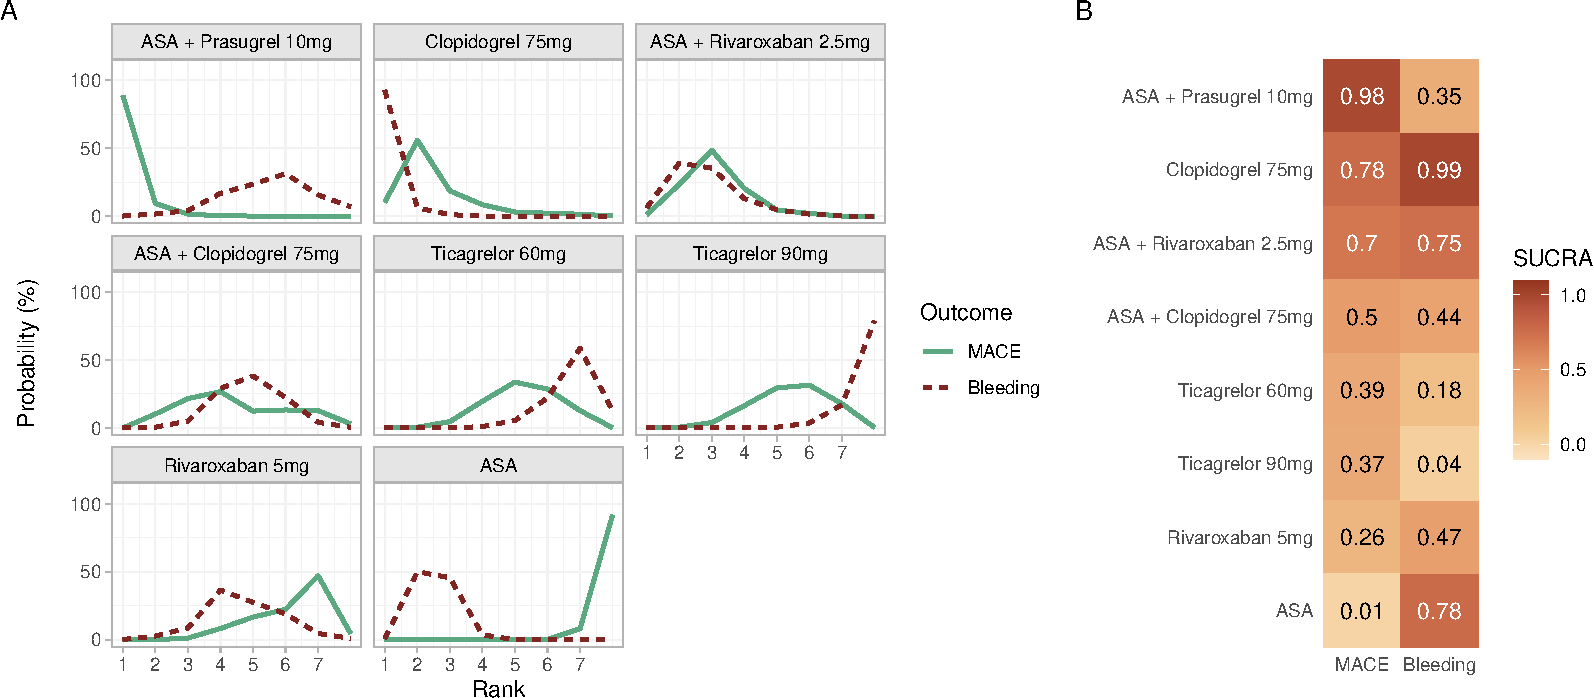
\includegraphics{03_supplementary_files/figure-latex/unnamed-chunk-29-1} \end{center}

Panel A: Ranking probabilities for MACE (solid line) and Bleeding
(dotted line) outcomes for each treatment. Panel B: Heatmap with
corresponding SUCRA values. While each row corresponds to a treatment,
each column depicts one outcome.

\end{landscape}

\hypertarget{efigure-6-ranks-with-uncertainty}{%
\subsection{eFigure 6: Ranks with
Uncertainty}\label{efigure-6-ranks-with-uncertainty}}

\begin{center}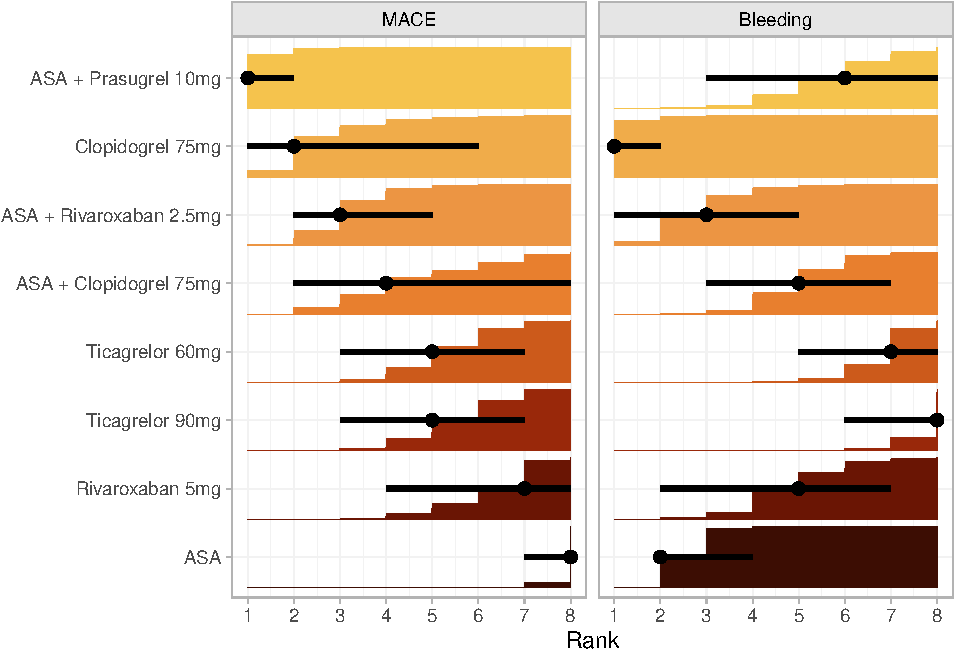
\includegraphics{03_supplementary_files/figure-latex/unnamed-chunk-30-1} \end{center}

Marginal posterior distributions for the rank of each treatment. Left
panel depicts ranks for MACE, while right panel for the Bleeding
outcome. In each panel, there are a point estimate, interval bar, and
bar plot for each treatment (Y-axis). The point estimate represents the
median rank. The interval bar shows the 95\% credible interval of the
underlying marginal posterior distribution. Lastly, the bar plot shows
the cumulative distribution function (CDF).

\newpage

\hypertarget{pooled-ticagrelor-networks-secondary-outcomes}{%
\section{Pooled Ticagrelor Networks: Secondary
Outcomes}\label{pooled-ticagrelor-networks-secondary-outcomes}}

\hypertarget{efigure-7-network-plots}{%
\subsection{eFigure 7: Network Plots}\label{efigure-7-network-plots}}

\textbf{Acute Myocardial Infarction}

\begin{center}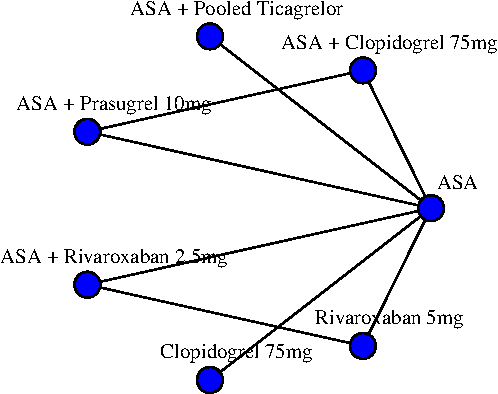
\includegraphics{03_supplementary_files/figure-latex/unnamed-chunk-31-1} \end{center}

\textbf{Ischemic Stroke, All-cause Mortality, and Cardiovascular Mortality}

\begin{center}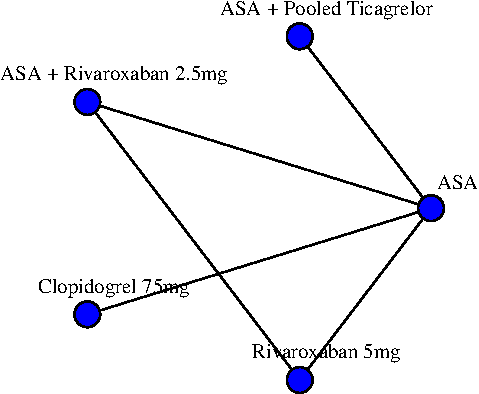
\includegraphics{03_supplementary_files/figure-latex/unnamed-chunk-32-1} \end{center}

\newpage

\hypertarget{efigure-8-forest-plot}{%
\subsection{eFigure 8: Forest Plot}\label{efigure-8-forest-plot}}

\begin{center}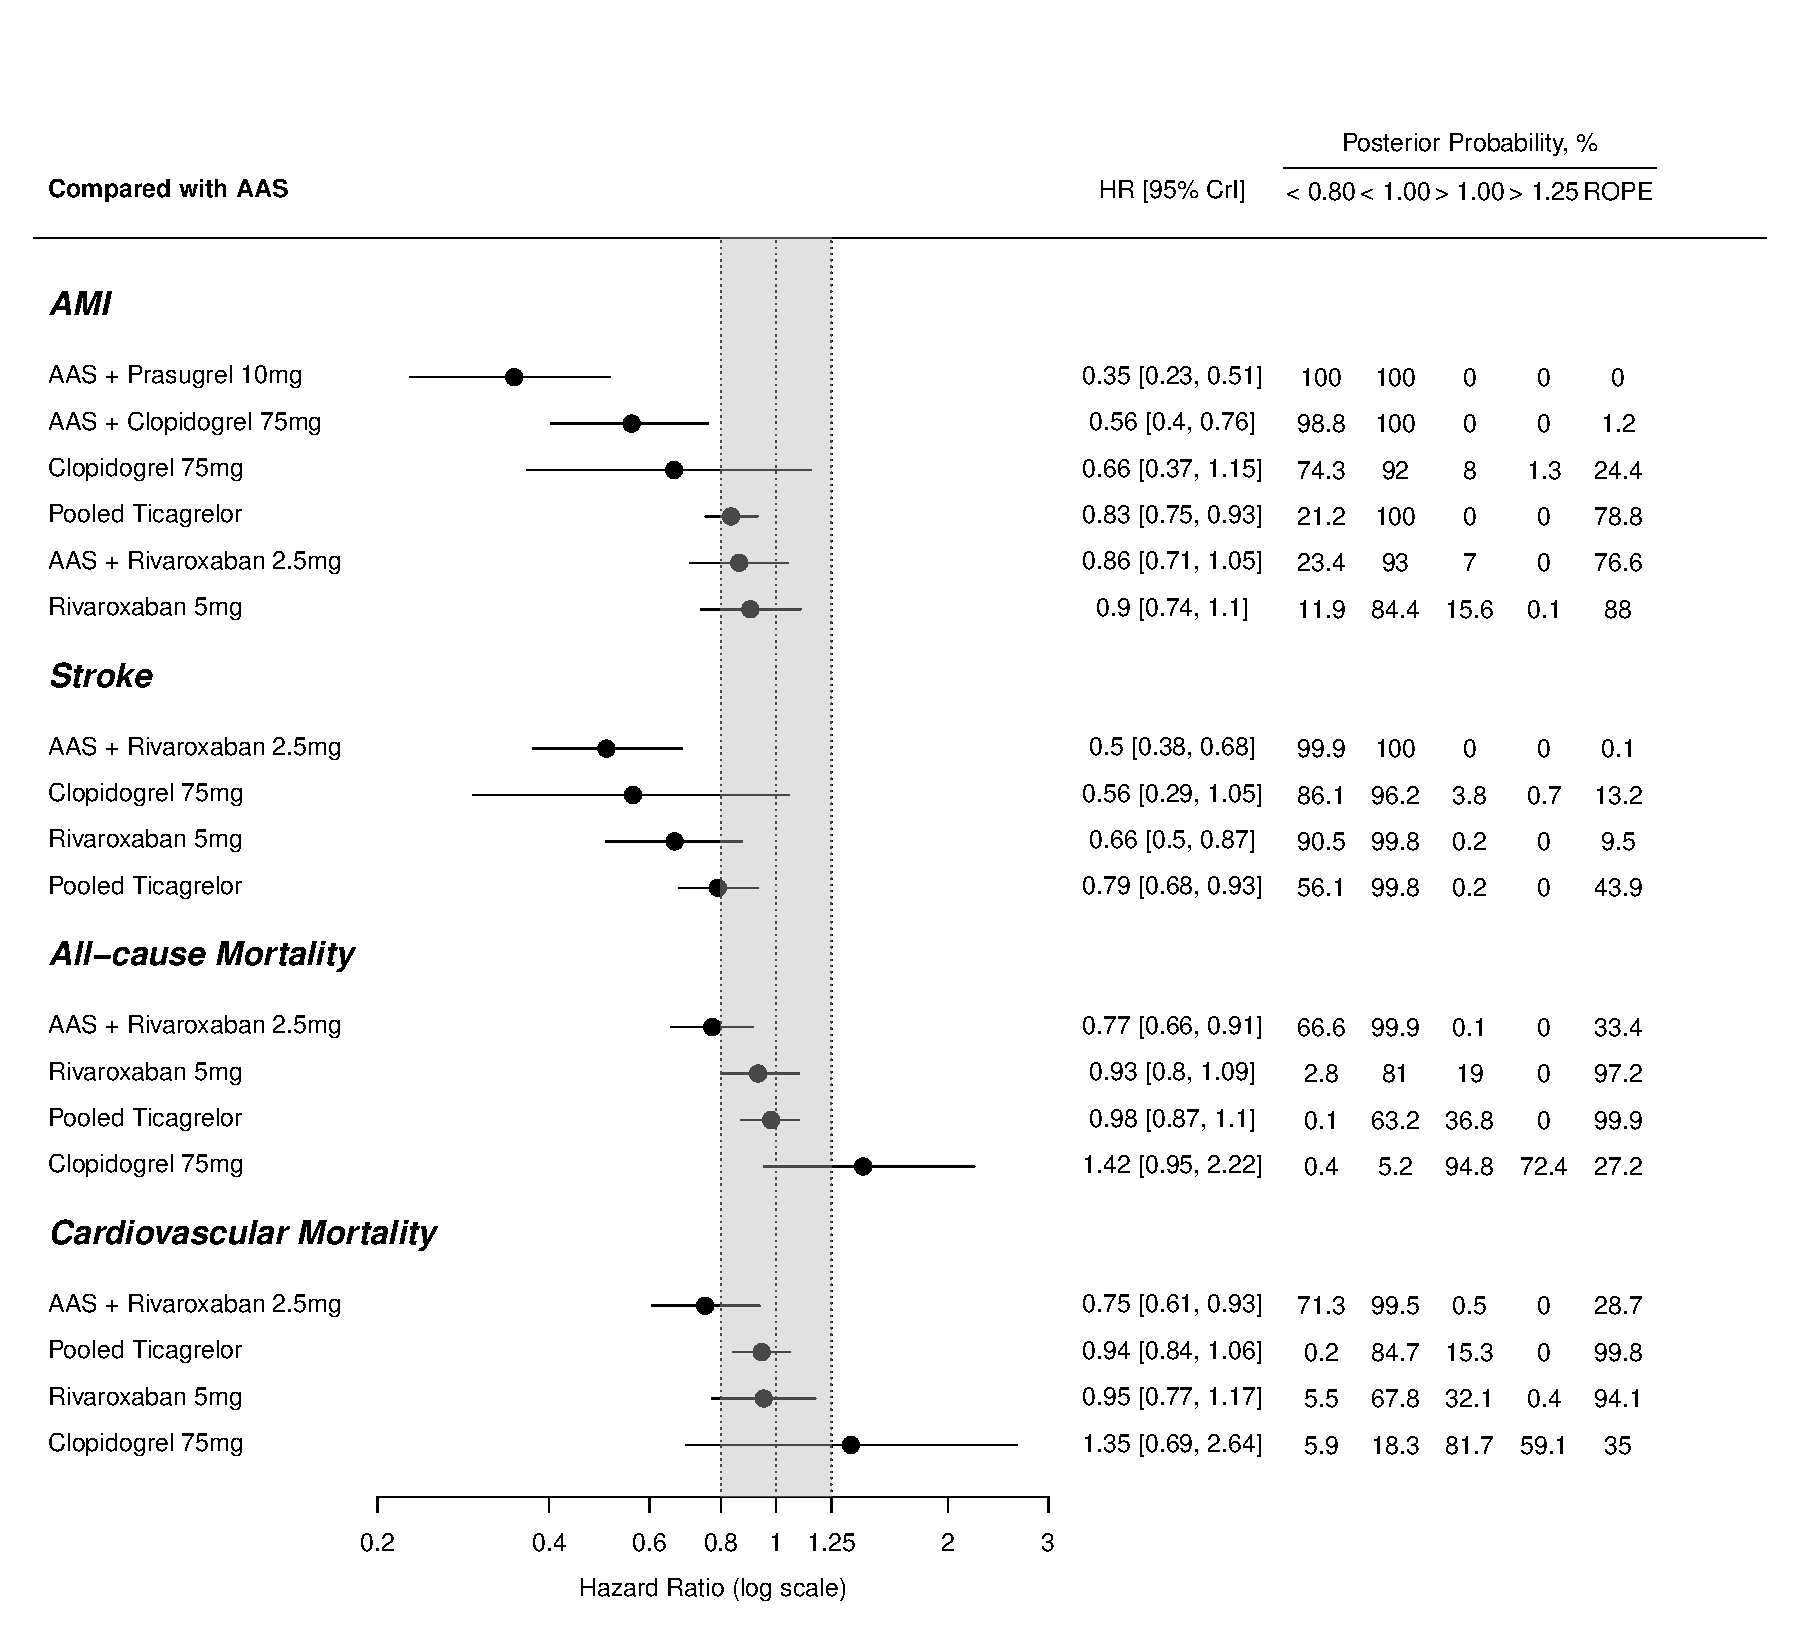
\includegraphics[width=1.1\linewidth]{/Users/arthur/Coding/projects/active/ARICOCAD_nma/output/plots/supplementary/forest_secondary_outcomes} \end{center}

Treatment effects compared to ASA on MACE and Bleeding outcomes, ordered
according to underlying SUCRA values. HR below 1.0 favors the
experimental treatment. On the left, treatment names are depicted. In
the middle, forest plot shows each treatment effect median and 95\%
credible intervals. Gray area corresponds to the ROPE (from 0.8 to 1.25
HR). On the right, exact effect sizes along with posterior probabilities
are shown.

Abbreviations: ROPE, region of practical equivalence; HR, hazard ratio.

\newpage

\begin{landscape}

\hypertarget{league-tables-2}{%
\subsection{League Tables}\label{league-tables-2}}

\hypertarget{etables-13-15-median-and-95-credible-intervals}{%
\subsubsection{eTables 13-15: Median and 95\% Credible
Intervals}\label{etables-13-15-median-and-95-credible-intervals}}

\begin{table}[!h]

\caption{\label{tab:unnamed-chunk-35}Acute Myocardial Infarction}
\centering
\resizebox{\linewidth}{!}{
\begin{tabular}[t]{lllllll}
\toprule
  &   &   &   &   &   &  \\
\midrule
ASA & 0.90 (0.74, 1.10) & 0.66 (0.37, 1.15) & 0.86 (0.71, 1.05) & 0.35 (0.23, 0.51) & 0.56 (0.40, 0.76) & 0.83 (0.75, 0.93)\\
 & Rivaroxaban 5mg & 0.73 (0.40, 1.35) & 0.96 (0.79, 1.17) & 0.38 (0.25, 0.60) & 0.62 (0.43, 0.90) & 0.93 (0.75, 1.16)\\
 &  & Clopidogrel 75mg & 1.30 (0.73, 2.44) & 0.53 (0.26, 1.04) & 0.84 (0.45, 1.65) & 1.26 (0.71, 2.32)\\
 &  &  & ASA + Rivaroxaban 2.5mg & 0.40 (0.26, 0.64) & 0.65 (0.44, 0.94) & 0.97 (0.77, 1.20)\\
 &  &  &  & ASA + Prasugrel 10mg & 1.60 (1.13, 2.21) & 2.40 (1.57, 3.59)\\
\addlinespace
 &  &  &  &  & ASA + Clopidogrel 75mg & 1.49 (1.07, 2.10)\\
 &  &  &  &  &  & Pooled Ticagrelor\\
\bottomrule
\end{tabular}}
\end{table}

Hazard ratios (95\% credible interval) for the Acute Myocardial
Infarction outcome. Treatments are shown in the diagonal. Comparisons
between treatments should be read from left to right and the estimate is
in the cell in common between the column-defining treatment and the
row-defining treatment. A hazard ratio \textless{} 1.0 favors the
column-defining treatment. For example, in the Rivaroxaban 5mg vs.~ASA
comparison, the corresponding HR (95\% CrI) was 0.90 (0.74, 1.10),
favoring Rivaroxaban 5mg (ie, HR \textless{} 1.0).

\end{landscape}

\begin{table}[!h]

\caption{\label{tab:unnamed-chunk-36}Ischemic Stroke}
\centering
\resizebox{\linewidth}{!}{
\begin{tabular}[t]{lllll}
\toprule
  &   &   &   &  \\
\midrule
ASA & 0.66 (0.50, 0.87) & 0.56 (0.29, 1.05) & 0.50 (0.38, 0.68) & 0.79 (0.68, 0.93)\\
 & Rivaroxaban 5mg & 0.84 (0.43, 1.67) & 0.76 (0.56, 1.00) & 1.19 (0.87, 1.63)\\
 &  & Clopidogrel 75mg & 0.90 (0.45, 1.80) & 1.41 (0.73, 2.68)\\
 &  &  & ASA + Rivaroxaban 2.5mg & 1.57 (1.13, 2.20)\\
 &  &  &  & Pooled Ticagrelor\\
\bottomrule
\end{tabular}}
\end{table}

Hazard ratios (95\% credible interval) for the Ischemic Stroke outcome.
Treatments are shown in the diagonal. Comparisons between treatments
should be read from left to right and the estimate is in the cell in
common between the column-defining treatment and the row-defining
treatment. A hazard ratio \textless{} 1.0 favors the column-defining
treatment. For example, in the Rivaroxaban 5mg vs.~ASA comparison, the
corresponding HR (95\% CrI) was 0.66 (0.50, 0.87), favoring Rivaroxaban
5mg (ie, HR \textless{} 1.0).

\begin{table}[!h]

\caption{\label{tab:unnamed-chunk-37}All-cause and Cardiovascular Mortality}
\centering
\resizebox{\linewidth}{!}{
\begin{tabular}[t]{lllll}
\toprule
  &   &   &   &  \\
\midrule
ASA & 0.93 (0.80, 1.09) & 1.42 (0.95, 2.22) & 0.77 (0.66, 0.91) & 0.98 (0.87, 1.10)\\
0.95 (0.77, 1.17) & Rivaroxaban 5mg & 1.52 (0.98, 2.41) & 0.83 (0.71, 0.98) & 1.05 (0.87, 1.28)\\
1.35 (0.69, 2.64) & 1.42 (0.71, 2.82) & Clopidogrel 75mg & 0.54 (0.35, 0.85) & 0.69 (0.44, 1.07)\\
0.75 (0.61, 0.93) & 0.79 (0.63, 0.97) & 0.56 (0.28, 1.12) & ASA + Rivaroxaban 2.5mg & 1.27 (1.03, 1.55)\\
0.94 (0.84, 1.06) & 0.99 (0.79, 1.27) & 0.70 (0.36, 1.37) & 1.26 (0.97, 1.60) & Pooled Ticagrelor\\
\bottomrule
\end{tabular}}
\end{table}

Hazard ratios (95\% credible interval) for the All-cause or
Cardiovascular mortality outcomes. Treatments are shown in the diagonal.
Results to the right of this diagonal (right upper half table)
correspond to the All-cause mortality outcome. Results to the left (left
lower half table) correspond to the Cardiovascular mortality outcome.
Comparisons between treatments should be read from left to right and the
estimate is in the cell in common between the column-defining treatment
and the row-defining treatment. For both outcomes, a hazard ratio
\textless{} 1.0 favors the column-defining treatment. For example, in
the Rivaroxaban 5mg vs.~ASA comparison for All-cause mortality, the
corresponding HR (95\% CrI) was 0.93 (0.80, 1.09), favoring Rivaroxaban
5mg (ie, HR \textless{} 1.0).

\newpage

\begin{landscape}

\hypertarget{etables-16-18-posterior-probabilities-of-hazard-ratio-1.0}{%
\subsubsection{eTables 16-18: Posterior Probabilities of Hazard Ratio
\textless{}
1.0}\label{etables-16-18-posterior-probabilities-of-hazard-ratio-1.0}}

\begin{table}[!h]

\caption{\label{tab:unnamed-chunk-38}Acute Myocardial Infarction}
\centering
\resizebox{\linewidth}{!}{
\begin{tabular}[t]{lllllll}
\toprule
  &   &   &   &   &   &  \\
\midrule
ASA & 84.41 & 91.96 & 93.05 & 100.00 & 99.99 & 99.99\\
 & Rivaroxaban 5mg & 84.44 & 66.90 & 100.00 & 99.49 & 75.36\\
 &  & Clopidogrel 75mg & 19.30 & 96.45 & 69.55 & 21.73\\
 &  &  & ASA + Rivaroxaban 2.5mg & 100.00 & 98.88 & 60.91\\
 &  &  &  & ASA + Prasugrel 10mg & 0.34 & 0.00\\
\addlinespace
 &  &  &  &  & ASA + Clopidogrel 75mg & 0.84\\
 &  &  &  &  &  & Pooled Ticagrelor\\
\bottomrule
\end{tabular}}
\end{table}

Posterior probabilities (\%) of hazard ratio \textless{} 1.0 for the
Acute Myocardial Infarction outcome. Treatments are shown in the
diagonal. Comparisons between treatments should be read from left to
right and the estimate is in the cell in common between the
column-defining treatment and the row-defining treatment. A hazard ratio
\textless{} 1.0 favors the column-defining treatment. For example, in
the Rivaroxaban 5mg vs.~ASA comparison, there was a posterior
probability of 84.41\% that the hazard ratio is below 1.0 (ie, there was
a 84.41\% probability for Rivaroxaban 5mg superiority).

\end{landscape}

\begin{table}[!h]

\caption{\label{tab:unnamed-chunk-39}Ischemic Stroke}
\centering
\resizebox{\linewidth}{!}{
\begin{tabular}[t]{lllll}
\toprule
  &   &   &   &  \\
\midrule
ASA & 99.78 & 96.21 & 100.00 & 99.84\\
 & Rivaroxaban 5mg & 67.96 & 96.91 & 14.72\\
 &  & Clopidogrel 75mg & 61.85 & 15.14\\
 &  &  & ASA + Rivaroxaban 2.5mg & 0.47\\
 &  &  &  & Pooled Ticagrelor\\
\bottomrule
\end{tabular}}
\end{table}

Posterior probabilities (\%) of hazard ratio \textless{} 1.0 for the
Ischemic Stroke outcome. Treatments are shown in the diagonal.
Comparisons between treatments should be read from left to right and the
estimate is in the cell in common between the column-defining treatment
and the row-defining treatment. A hazard ratio \textless{} 1.0 favors
the column-defining treatment. For example, in the Rivaroxaban 5mg
vs.~ASA comparison, there was a posterior probability of 99.78\% that
the hazard ratio is below 1.0 (ie, there was a 99.78\% probability for
Rivaroxaban 5mg superiority).

\begin{table}[!h]

\caption{\label{tab:unnamed-chunk-40}All-cause and Cardiovascular Mortality}
\centering
\resizebox{\linewidth}{!}{
\begin{tabular}[t]{lllll}
\toprule
  &   &   &   &  \\
\midrule
ASA & 81.00 & 5.22 & 99.88 & 63.21\\
67.85 & Rivaroxaban 5mg & 3.20 & 99.01 & 31.13\\
18.30 & 15.59 & Clopidogrel 75mg & 99.55 & 95.09\\
99.51 & 98.32 & 95.00 & ASA + Rivaroxaban 2.5mg & 1.09\\
84.67 & 52.39 & 85.71 & 3.71 & Pooled Ticagrelor\\
\bottomrule
\end{tabular}}
\end{table}

Posterior probabilities (\%) of hazard ratio \textless{} 1.0 for the
All-cause or Cardiovascular mortality outcomes. Treatments are shown in
the diagonal. Results to the right of this diagonal (right upper half
table) correspond to the All-cause mortality outcome. Results to the
left (left lower half table) correspond to the Cardiovascular mortality
outcome. Comparisons between treatments should be read from left to
right and the estimate is in the cell in common between the
column-defining treatment and the row-defining treatment. For both
outcomes, a hazard ratio \textless{} 1.0 favors the column-defining
treatment. For example, in the Rivaroxaban 5mg vs.~ASA comparison for
All-cause mortality, there was a posterior probability of 81.00\% that
the hazard ratio is below 1.0 (ie, there was a 81.00\% probability for
Rivaroxaban 5mg superiority).

\newpage

\begin{landscape}

\hypertarget{etables-19-21-posterior-probabilities-of-hazard-ratio-0.8}{%
\subsubsection{eTables 19-21: Posterior Probabilities of Hazard Ratio
\textless{}
0.8}\label{etables-19-21-posterior-probabilities-of-hazard-ratio-0.8}}

\begin{table}[!h]

\caption{\label{tab:unnamed-chunk-41}Acute Myocardial Infarction}
\centering
\resizebox{\linewidth}{!}{
\begin{tabular}[t]{lllllll}
\toprule
  &   &   &   &   &   &  \\
\midrule
ASA & 11.95 & 74.31 & 23.38 & 100.00 & 98.76 & 21.18\\
 & Rivaroxaban 5mg & 61.42 & 4.20 & 99.96 & 91.38 & 10.10\\
 &  & Clopidogrel 75mg & 5.47 & 87.78 & 43.68 & 6.42\\
 &  &  & ASA + Rivaroxaban 2.5mg & 99.92 & 86.95 & 4.42\\
 &  &  &  & ASA + Prasugrel 10mg & 0.01 & 0.00\\
\addlinespace
 &  &  &  &  & ASA + Clopidogrel 75mg & 0.00\\
 &  &  &  &  &  & Pooled Ticagrelor\\
\bottomrule
\end{tabular}}
\end{table}

Posterior probabilities (\%) of hazard ratio \textless{} 0.80 for the
Acute Myocardial Infarction outcome. Treatments are shown in the
diagonal. Comparisons between treatments should be read from left to
right and the estimate is in the cell in common between the
column-defining treatment and the row-defining treatment. A hazard ratio
\textless{} 1.0 favors the column-defining treatment. For example, in
the Rivaroxaban 5mg vs.~ASA comparison, there was a posterior
probability of 11.95\% that the hazard ratio is below 0.80.

\end{landscape}

\begin{table}[!h]

\caption{\label{tab:unnamed-chunk-42}Ischemic Stroke}
\centering
\resizebox{\linewidth}{!}{
\begin{tabular}[t]{lllll}
\toprule
  &   &   &   &  \\
\midrule
ASA & 90.46 & 86.09 & 99.90 & 56.12\\
 & Rivaroxaban 5mg & 44.45 & 63.78 & 0.69\\
 &  & Clopidogrel 75mg & 37.50 & 4.54\\
 &  &  & ASA + Rivaroxaban 2.5mg & 0.00\\
 &  &  &  & Pooled Ticagrelor\\
\bottomrule
\end{tabular}}
\end{table}

Posterior probabilities (\%) of hazard ratio \textless{} 0.80 for the
Ischemic Stroke outcome. Treatments are shown in the diagonal.
Comparisons between treatments should be read from left to right and the
estimate is in the cell in common between the column-defining treatment
and the row-defining treatment. A hazard ratio \textless{} 1.0 favors
the column-defining treatment. For example, in the Rivaroxaban 5mg
vs.~ASA comparison, there was a posterior probability of 90.46\% that
the hazard ratio is below 0.80.

\begin{table}[!h]

\caption{\label{tab:unnamed-chunk-43}All-cause and Cardiovascular Mortality}
\centering
\resizebox{\linewidth}{!}{
\begin{tabular}[t]{lllll}
\toprule
  &   &   &   &  \\
\midrule
ASA & 2.84 & 0.35 & 66.61 & 0.09\\
5.51 & Rivaroxaban 5mg & 0.26 & 33.65 & 0.43\\
5.90 & 5.30 & Clopidogrel 75mg & 95.43 & 74.46\\
71.29 & 54.85 & 85.20 & ASA + Rivaroxaban 2.5mg & 0.00\\
0.24 & 4.01 & 65.56 & 0.00 & Pooled Ticagrelor\\
\bottomrule
\end{tabular}}
\end{table}

Posterior probabilities (\%) of hazard ratio \textless{} 0.80 for the
All-cause or Cardiovascular mortality outcomes. Treatments are shown in
the diagonal. Results to the right of this diagonal (right upper half
table) correspond to the All-cause mortality outcome. Results to the
left (left lower half table) correspond to the Cardiovascular mortality
outcome. Comparisons between treatments should be read from left to
right and the estimate is in the cell in common between the
column-defining treatment and the row-defining treatment. For both
outcomes, a hazard ratio \textless{} 1.0 favors the column-defining
treatment. For example, in the Rivaroxaban 5mg vs.~ASA comparison for
All-cause mortality, there was a posterior probability of 2.84\% that
the hazard ratio is below 0.80.

\newpage

\begin{landscape}

\hypertarget{etables-22-24-posterior-probabilities-of-hazard-ratio-1.25}{%
\subsubsection{eTables 22-24: Posterior Probabilities of Hazard Ratio
\textgreater{}
1.25}\label{etables-22-24-posterior-probabilities-of-hazard-ratio-1.25}}

\begin{table}[!h]

\caption{\label{tab:unnamed-chunk-44}Acute Myocardial Infarction}
\centering
\resizebox{\linewidth}{!}{
\begin{tabular}[t]{lllllll}
\toprule
  &   &   &   &   &   &  \\
\midrule
ASA & 0.06 & 1.32 & 0.00 & 0.00 & 0.00 & 0.00\\
 & Rivaroxaban 5mg & 4.19 & 0.35 & 0.00 & 0.01 & 0.41\\
 &  & Clopidogrel 75mg & 55.04 & 0.91 & 11.80 & 51.45\\
 &  &  & ASA + Rivaroxaban 2.5mg & 0.00 & 0.04 & 1.20\\
 &  &  &  & ASA + Prasugrel 10mg & 92.62 & 99.90\\
\addlinespace
 &  &  &  &  & ASA + Clopidogrel 75mg & 85.66\\
 &  &  &  &  &  & Pooled Ticagrelor\\
\bottomrule
\end{tabular}}
\end{table}

Posterior probabilities (\%) of hazard ratio \textgreater{} 1.25 for the
Acute Myocardial Infarction outcome. Treatments are shown in the
diagonal. Comparisons between treatments should be read from left to
right and the estimate is in the cell in common between the
column-defining treatment and the row-defining treatment. For both
outcomes, a hazard ratio \textless{} 1.0 favors the column-defining
treatment. For example, in the Rivaroxaban 5mg vs.~ASA comparison, there
was a posterior probability of 0.06\% that the hazard ratio is above
1.25.

\end{landscape}

\begin{table}[!h]

\caption{\label{tab:unnamed-chunk-45}Ischemic Stroke}
\centering
\resizebox{\linewidth}{!}{
\begin{tabular}[t]{lllll}
\toprule
  &   &   &   &  \\
\midrule
ASA & 0.00 & 0.66 & 0.00 & 0.00\\
 & Rivaroxaban 5mg & 13.48 & 0.00 & 38.48\\
 &  & Clopidogrel 75mg & 18.57 & 64.20\\
 &  &  & ASA + Rivaroxaban 2.5mg & 90.22\\
 &  &  &  & Pooled Ticagrelor\\
\bottomrule
\end{tabular}}
\end{table}

Posterior probabilities (\%) of hazard ratio \textgreater{} 1.25 for the
Ischemic Stroke outcome. Treatments are shown in the diagonal.
Comparisons between treatments should be read from left to right and the
estimate is in the cell in common between the column-defining treatment
and the row-defining treatment. For both outcomes, a hazard ratio
\textless{} 1.0 favors the column-defining treatment. For example, in
the Rivaroxaban 5mg vs.~ASA comparison, there was a posterior
probability of 0.00\% that the hazard ratio is above 1.25.

\begin{table}[!h]

\caption{\label{tab:unnamed-chunk-46}All-cause and Cardiovascular Mortality}
\centering
\resizebox{\linewidth}{!}{
\begin{tabular}[t]{lllll}
\toprule
  &   &   &   &  \\
\midrule
ASA & 0.00 & 72.41 & 0.00 & 0.00\\
0.41 & Rivaroxaban 5mg & 80.41 & 0.00 & 3.99\\
59.11 & 64.08 & Clopidogrel 75mg & 0.00 & 0.41\\
0.00 & 0.00 & 1.29 & ASA + Rivaroxaban 2.5mg & 56.09\\
0.00 & 3.02 & 4.54 & 51.69 & Pooled Ticagrelor\\
\bottomrule
\end{tabular}}
\end{table}

Posterior probabilities (\%) of hazard ratio \textgreater{} 1.25 for the
All-cause or Cardiovascular mortality outcomes. Treatments are shown in
the diagonal. Results to the right of this diagonal (right upper half
table) correspond to the All-cause mortality outcome. Results to the
left (left lower half table) correspond to the Cardiovascular mortality
outcome. Comparisons between treatments should be read from left to
right and the estimate is in the cell in common between the
column-defining treatment and the row-defining treatment. For both
outcomes, a hazard ratio \textless{} 1.0 favors the column-defining
treatment. For example, in the Rivaroxaban 5mg vs.~ASA comparison for
MACE, there was a posterior probability of 0.00\% that the hazard ratio
is above 1.25.

\newpage

\begin{landscape}

\hypertarget{etables-25-27-posterior-probabilities-of-hazard-ratio-within-the-rope}{%
\subsubsection{eTables 25-27: Posterior Probabilities of Hazard Ratio
within the
ROPE}\label{etables-25-27-posterior-probabilities-of-hazard-ratio-within-the-rope}}

\begin{table}[!h]

\caption{\label{tab:unnamed-chunk-47}Acute Myocardial Infarction}
\centering
\resizebox{\linewidth}{!}{
\begin{tabular}[t]{lllllll}
\toprule
  &   &   &   &   &   &  \\
\midrule
ASA & 87.99 & 24.36 & 76.62 & 0.00 & 1.24 & 78.83\\
 & Rivaroxaban 5mg & 34.39 & 95.45 & 0.04 & 8.61 & 89.49\\
 &  & Clopidogrel 75mg & 39.49 & 11.31 & 44.52 & 42.12\\
 &  &  & ASA + Rivaroxaban 2.5mg & 0.07 & 13.01 & 94.38\\
 &  &  &  & ASA + Prasugrel 10mg & 7.36 & 0.10\\
\addlinespace
 &  &  &  &  & ASA + Clopidogrel 75mg & 14.34\\
 &  &  &  &  &  & Pooled Ticagrelor\\
\bottomrule
\end{tabular}}
\end{table}

Posterior probabilities (\%) of hazard ratio within the region of
practical equivalence (ROPE), ie, between 0.80 and 1.25, for the Acute
Myocardial Infarction outcome. Treatments are shown in the diagonal.
Comparisons between treatments should be read from left to right and the
estimate is in the cell in common between the column-defining treatment
and the row-defining treatment. For both outcomes, a hazard ratio
\textless{} 1.0 favors the column-defining treatment. For example, in
the Rivaroxaban 5mg vs.~ASA comparison, there was a posterior
probability of 87.99\% that the hazard ratio is within the ROPE.

\end{landscape}

\begin{table}[!h]

\caption{\label{tab:unnamed-chunk-48}Ischemic Stroke}
\centering
\resizebox{\linewidth}{!}{
\begin{tabular}[t]{lllll}
\toprule
  &   &   &   &  \\
\midrule
ASA & 9.54 & 13.25 & 0.10 & 43.88\\
 & Rivaroxaban 5mg & 42.08 & 36.23 & 60.84\\
 &  & Clopidogrel 75mg & 43.92 & 31.26\\
 &  &  & ASA + Rivaroxaban 2.5mg & 9.78\\
 &  &  &  & Pooled Ticagrelor\\
\bottomrule
\end{tabular}}
\end{table}

Posterior probabilities (\%) of hazard ratio within the region of
practical equivalence (ROPE), ie, between 0.80 and 1.25, for the
Ischemic Stroke outcome. Treatments are shown in the diagonal.
Comparisons between treatments should be read from left to right and the
estimate is in the cell in common between the column-defining treatment
and the row-defining treatment. For both outcomes, a hazard ratio
\textless{} 1.0 favors the column-defining treatment. For example, in
the Rivaroxaban 5mg vs.~ASA comparison, there was a posterior
probability of 9.54\% that the hazard ratio is within the ROPE.

\begin{table}[!h]

\caption{\label{tab:unnamed-chunk-49}All-cause and Cardiovascular Mortality}
\centering
\resizebox{\linewidth}{!}{
\begin{tabular}[t]{lllll}
\toprule
  &   &   &   &  \\
\midrule
ASA & 97.16 & 27.24 & 33.39 & 99.91\\
67.85 & Rivaroxaban 5mg & 19.32 & 66.35 & 95.59\\
18.30 & 15.59 & Clopidogrel 75mg & 4.58 & 25.12\\
99.51 & 98.32 & 95.00 & ASA + Rivaroxaban 2.5mg & 43.91\\
84.67 & 52.39 & 85.71 & 3.71 & Pooled Ticagrelor\\
\bottomrule
\end{tabular}}
\end{table}

Posterior probabilities (\%) of hazard ratio within the region of
practical equivalence (ROPE), ie, between 0.80 and 1.25, for the
All-cause or Cardiovascular mortality outcomes. Treatments are shown in
the diagonal. Results to the right of this diagonal (right upper half
table) correspond to the All-cause mortality outcome. Results to the
left (left lower half table) correspond to the Cardiovascular mortality
outcome. Comparisons between treatments should be read from left to
right and the estimate is in the cell in common between the
column-defining treatment and the row-defining treatment. For both
outcomes, a hazard ratio \textless{} 1.0 favors the column-defining
treatment. For example, in the Rivaroxaban 5mg vs.~ASA comparison for
All-cause mortality, there was a posterior probability of 97.16\% that
the hazard ratio is within the ROPE.

\newpage

\begin{landscape}

\hypertarget{efigure-9-ranks-sucra}{%
\subsection{eFigure 9: Ranks + SUCRA}\label{efigure-9-ranks-sucra}}

\begin{center}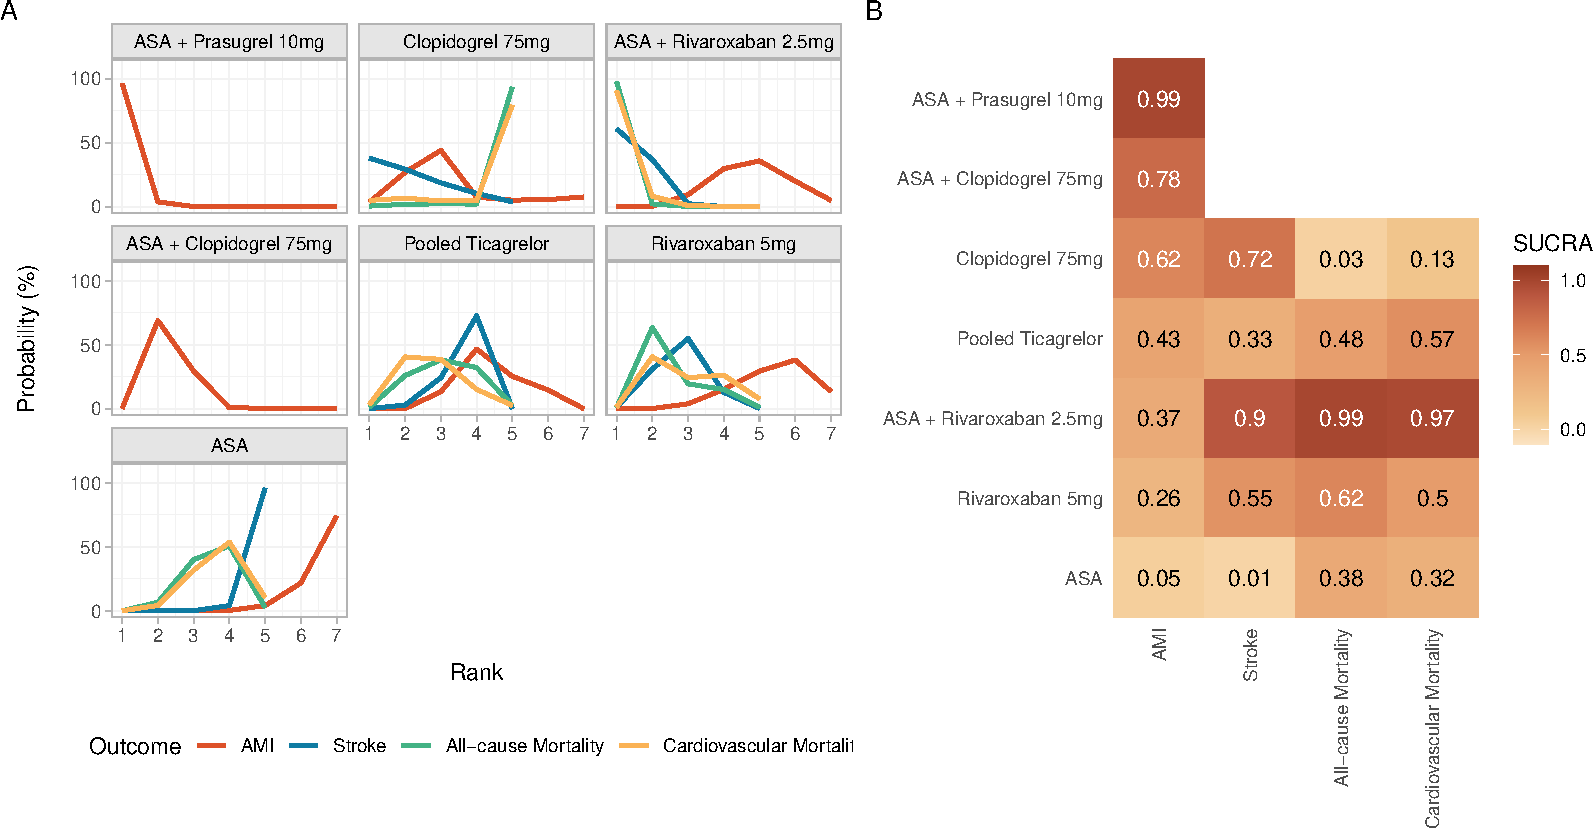
\includegraphics{03_supplementary_files/figure-latex/unnamed-chunk-52-1} \end{center}

Panel A: Ranking probabilities for Acute Myocardical Infarction (AMI),
Stroke, All-cause and Cardiovascular Mortality outcomes for each
treatment. There are only AMI rankings for ``ASA + Prasugrel 10mg'' and
``ASA + Clopidogrel 75mg'' because there was no data available for other
outcomes in corresponding studies. Panel B: Heatmap with corresponding
SUCRA values. While each row corresponds to a treatment, each column
depicts one outcome.

\end{landscape}

\hypertarget{efigure-10-ranks-with-uncertainty}{%
\subsection{eFigure 10: Ranks with
Uncertainty}\label{efigure-10-ranks-with-uncertainty}}

\begin{center}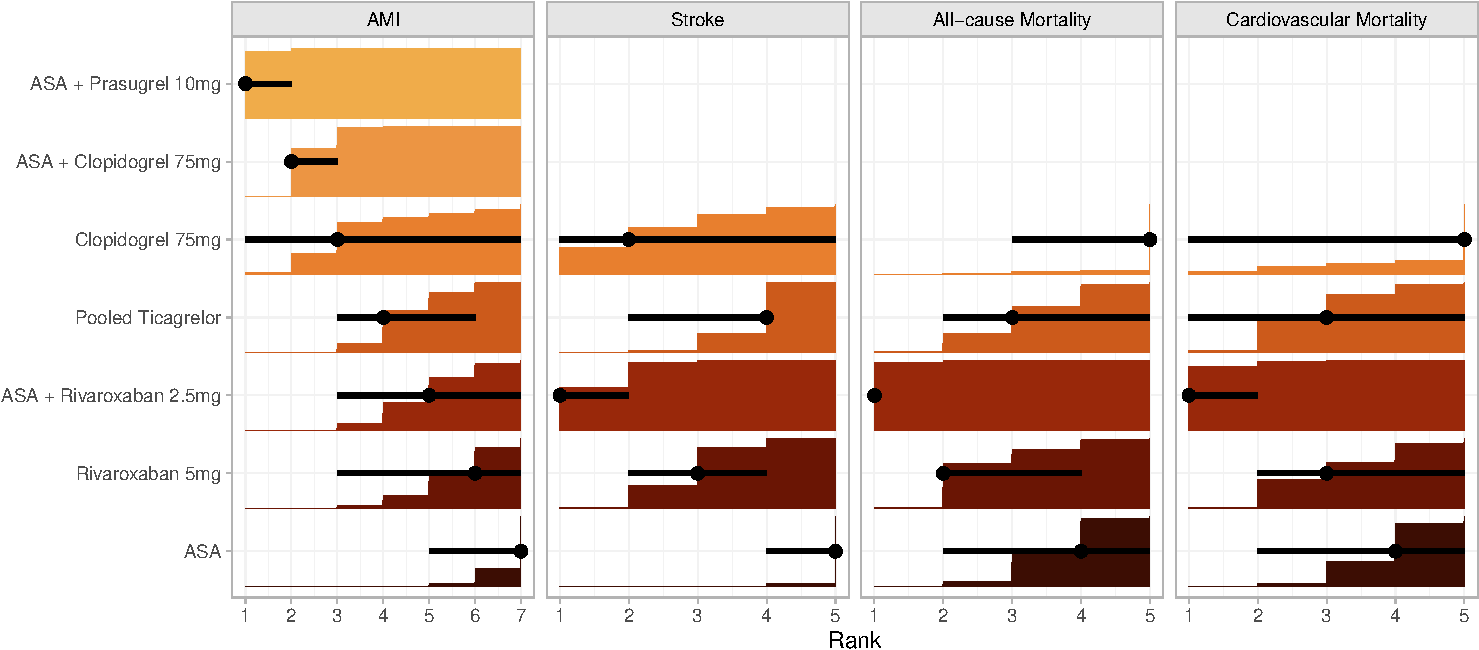
\includegraphics{03_supplementary_files/figure-latex/unnamed-chunk-53-1} \end{center}

Marginal posterior distributions for the rank of each treatment. Each
panel corresponds to a separate outcome, labeled on top. In each panel,
there are a point estimate, interval bar, and bar plot for each
treatment (Y-axis). The point estimate represents the median rank. The
interval bar shows the 95\% credible (quantile) interval of the
underlying marginal posterior distribution. Lastly, the bar plot shows
the cumulative distribution function (CDF).

\newpage

\begin{landscape}

\hypertarget{cinema}{%
\section{CINeMA}\label{cinema}}

\hypertarget{etables-28-33-pooled-ticagrelor-networks}{%
\subsection{eTables 28-33: Pooled Ticagrelor
Networks}\label{etables-28-33-pooled-ticagrelor-networks}}

\hypertarget{mace-1}{%
\subsubsection{MACE}\label{mace-1}}

\begin{table}[!h]
\centering
\resizebox{\linewidth}{!}{
\begin{tabular}[t]{llllllll}
\toprule
Comparison & Within-study bias & Reporting bias & Indirectness & Imprecision & Heterogeneity & Incoherence & Overall rating\\
\midrule
ASA vs. Rivaroxaban 5mg & \cellcolor[HTML]{5CA881}{\textcolor{white}{No concerns}} & \cellcolor[HTML]{E7B03C}{\textcolor{white}{Suspected}} & \cellcolor[HTML]{5CA881}{\textcolor{white}{No concerns}} & \cellcolor[HTML]{E7B03C}{\textcolor{white}{Some concerns}} & \cellcolor[HTML]{B5B5B5}{Not applicable} & \cellcolor[HTML]{EA4025}{\textcolor{white}{Major concerns}} & \cellcolor[HTML]{A32A31}{\textcolor{white}{Very Low}}\\
ASA vs. Clopidogrel 75mg & \cellcolor[HTML]{5CA881}{\textcolor{white}{No concerns}} & \cellcolor[HTML]{5CA881}{\textcolor{white}{Undetected}} & \cellcolor[HTML]{5CA881}{\textcolor{white}{No concerns}} & \cellcolor[HTML]{5CA881}{\textcolor{white}{No concerns}} & \cellcolor[HTML]{B5B5B5}{Not applicable} & \cellcolor[HTML]{EA4025}{\textcolor{white}{Major concerns}} & \cellcolor[HTML]{EA4025}{\textcolor{white}{Low}}\\
ASA vs. ASA + Rivaroxaban 2.5mg & \cellcolor[HTML]{5CA881}{\textcolor{white}{No concerns}} & \cellcolor[HTML]{E7B03C}{\textcolor{white}{Suspected}} & \cellcolor[HTML]{5CA881}{\textcolor{white}{No concerns}} & \cellcolor[HTML]{5CA881}{\textcolor{white}{No concerns}} & \cellcolor[HTML]{B5B5B5}{Not applicable} & \cellcolor[HTML]{EA4025}{\textcolor{white}{Major concerns}} & \cellcolor[HTML]{EA4025}{\textcolor{white}{Low}}\\
ASA vs. ASA + Prasugrel 10mg & \cellcolor[HTML]{5CA881}{\textcolor{white}{No concerns}} & \cellcolor[HTML]{5CA881}{\textcolor{white}{Undetected}} & \cellcolor[HTML]{5CA881}{\textcolor{white}{No concerns}} & \cellcolor[HTML]{5CA881}{\textcolor{white}{No concerns}} & \cellcolor[HTML]{B5B5B5}{Not applicable} & \cellcolor[HTML]{EA4025}{\textcolor{white}{Major concerns}} & \cellcolor[HTML]{EA4025}{\textcolor{white}{Low}}\\
ASA vs. ASA + Clopidogrel 75mg & \cellcolor[HTML]{5CA881}{\textcolor{white}{No concerns}} & \cellcolor[HTML]{5CA881}{\textcolor{white}{Undetected}} & \cellcolor[HTML]{5CA881}{\textcolor{white}{No concerns}} & \cellcolor[HTML]{5CA881}{\textcolor{white}{No concerns}} & \cellcolor[HTML]{B5B5B5}{Not applicable} & \cellcolor[HTML]{EA4025}{\textcolor{white}{Major concerns}} & \cellcolor[HTML]{EA4025}{\textcolor{white}{Low}}\\
\addlinespace
ASA vs. Pooled Ticagrelor & \cellcolor[HTML]{5CA881}{\textcolor{white}{No concerns}} & \cellcolor[HTML]{E7B03C}{\textcolor{white}{Suspected}} & \cellcolor[HTML]{5CA881}{\textcolor{white}{No concerns}} & \cellcolor[HTML]{5CA881}{\textcolor{white}{No concerns}} & \cellcolor[HTML]{B5B5B5}{Not applicable} & \cellcolor[HTML]{EA4025}{\textcolor{white}{Major concerns}} & \cellcolor[HTML]{EA4025}{\textcolor{white}{Low}}\\
Rivaroxaban 5mg vs. Clopidogrel 75mg & \cellcolor[HTML]{5CA881}{\textcolor{white}{No concerns}} & \cellcolor[HTML]{E7B03C}{\textcolor{white}{Suspected}} & \cellcolor[HTML]{5CA881}{\textcolor{white}{No concerns}} & \cellcolor[HTML]{E7B03C}{\textcolor{white}{Some concerns}} & \cellcolor[HTML]{B5B5B5}{Not applicable} & \cellcolor[HTML]{EA4025}{\textcolor{white}{Major concerns}} & \cellcolor[HTML]{A32A31}{\textcolor{white}{Very Low}}\\
Rivaroxaban 5mg vs. ASA + Rivaroxaban 2.5mg & \cellcolor[HTML]{5CA881}{\textcolor{white}{No concerns}} & \cellcolor[HTML]{E7B03C}{\textcolor{white}{Suspected}} & \cellcolor[HTML]{5CA881}{\textcolor{white}{No concerns}} & \cellcolor[HTML]{5CA881}{\textcolor{white}{No concerns}} & \cellcolor[HTML]{B5B5B5}{Not applicable} & \cellcolor[HTML]{EA4025}{\textcolor{white}{Major concerns}} & \cellcolor[HTML]{EA4025}{\textcolor{white}{Low}}\\
Rivaroxaban 5mg vs. ASA + Prasugrel 10mg & \cellcolor[HTML]{5CA881}{\textcolor{white}{No concerns}} & \cellcolor[HTML]{E7B03C}{\textcolor{white}{Suspected}} & \cellcolor[HTML]{5CA881}{\textcolor{white}{No concerns}} & \cellcolor[HTML]{5CA881}{\textcolor{white}{No concerns}} & \cellcolor[HTML]{B5B5B5}{Not applicable} & \cellcolor[HTML]{EA4025}{\textcolor{white}{Major concerns}} & \cellcolor[HTML]{EA4025}{\textcolor{white}{Low}}\\
Rivaroxaban 5mg vs. ASA + Clopidogrel 75mg & \cellcolor[HTML]{5CA881}{\textcolor{white}{No concerns}} & \cellcolor[HTML]{E7B03C}{\textcolor{white}{Suspected}} & \cellcolor[HTML]{5CA881}{\textcolor{white}{No concerns}} & \cellcolor[HTML]{E7B03C}{\textcolor{white}{Some concerns}} & \cellcolor[HTML]{B5B5B5}{Not applicable} & \cellcolor[HTML]{EA4025}{\textcolor{white}{Major concerns}} & \cellcolor[HTML]{A32A31}{\textcolor{white}{Very Low}}\\
\addlinespace
Rivaroxaban 5mg vs. Pooled Ticagrelor & \cellcolor[HTML]{5CA881}{\textcolor{white}{No concerns}} & \cellcolor[HTML]{E7B03C}{\textcolor{white}{Suspected}} & \cellcolor[HTML]{5CA881}{\textcolor{white}{No concerns}} & \cellcolor[HTML]{5CA881}{\textcolor{white}{No concerns}} & \cellcolor[HTML]{B5B5B5}{Not applicable} & \cellcolor[HTML]{EA4025}{\textcolor{white}{Major concerns}} & \cellcolor[HTML]{EA4025}{\textcolor{white}{Low}}\\
Clopidogrel 75mg vs. ASA + Rivaroxaban 2.5mg & \cellcolor[HTML]{5CA881}{\textcolor{white}{No concerns}} & \cellcolor[HTML]{E7B03C}{\textcolor{white}{Suspected}} & \cellcolor[HTML]{5CA881}{\textcolor{white}{No concerns}} & \cellcolor[HTML]{EA4025}{\textcolor{white}{Major concerns}} & \cellcolor[HTML]{B5B5B5}{Not applicable} & \cellcolor[HTML]{EA4025}{\textcolor{white}{Major concerns}} & \cellcolor[HTML]{A32A31}{\textcolor{white}{Very Low}}\\
Clopidogrel 75mg vs. ASA + Prasugrel 10mg & \cellcolor[HTML]{5CA881}{\textcolor{white}{No concerns}} & \cellcolor[HTML]{5CA881}{\textcolor{white}{Undetected}} & \cellcolor[HTML]{5CA881}{\textcolor{white}{No concerns}} & \cellcolor[HTML]{E7B03C}{\textcolor{white}{Some concerns}} & \cellcolor[HTML]{B5B5B5}{Not applicable} & \cellcolor[HTML]{EA4025}{\textcolor{white}{Major concerns}} & \cellcolor[HTML]{A32A31}{\textcolor{white}{Very Low}}\\
Clopidogrel 75mg vs. ASA + Clopidogrel 75mg & \cellcolor[HTML]{5CA881}{\textcolor{white}{No concerns}} & \cellcolor[HTML]{5CA881}{\textcolor{white}{Undetected}} & \cellcolor[HTML]{5CA881}{\textcolor{white}{No concerns}} & \cellcolor[HTML]{E7B03C}{\textcolor{white}{Some concerns}} & \cellcolor[HTML]{B5B5B5}{Not applicable} & \cellcolor[HTML]{EA4025}{\textcolor{white}{Major concerns}} & \cellcolor[HTML]{A32A31}{\textcolor{white}{Very Low}}\\
Clopidogrel 75mg vs. Pooled Ticagrelor & \cellcolor[HTML]{5CA881}{\textcolor{white}{No concerns}} & \cellcolor[HTML]{E7B03C}{\textcolor{white}{Suspected}} & \cellcolor[HTML]{5CA881}{\textcolor{white}{No concerns}} & \cellcolor[HTML]{E7B03C}{\textcolor{white}{Some concerns}} & \cellcolor[HTML]{B5B5B5}{Not applicable} & \cellcolor[HTML]{EA4025}{\textcolor{white}{Major concerns}} & \cellcolor[HTML]{A32A31}{\textcolor{white}{Very Low}}\\
\addlinespace
ASA + Rivaroxaban 2.5mg vs. ASA + Prasugrel 10mg & \cellcolor[HTML]{5CA881}{\textcolor{white}{No concerns}} & \cellcolor[HTML]{E7B03C}{\textcolor{white}{Suspected}} & \cellcolor[HTML]{5CA881}{\textcolor{white}{No concerns}} & \cellcolor[HTML]{5CA881}{\textcolor{white}{No concerns}} & \cellcolor[HTML]{B5B5B5}{Not applicable} & \cellcolor[HTML]{EA4025}{\textcolor{white}{Major concerns}} & \cellcolor[HTML]{EA4025}{\textcolor{white}{Low}}\\
ASA + Rivaroxaban 2.5mg vs. ASA + Clopidogrel 75mg & \cellcolor[HTML]{5CA881}{\textcolor{white}{No concerns}} & \cellcolor[HTML]{E7B03C}{\textcolor{white}{Suspected}} & \cellcolor[HTML]{5CA881}{\textcolor{white}{No concerns}} & \cellcolor[HTML]{E7B03C}{\textcolor{white}{Some concerns}} & \cellcolor[HTML]{B5B5B5}{Not applicable} & \cellcolor[HTML]{EA4025}{\textcolor{white}{Major concerns}} & \cellcolor[HTML]{A32A31}{\textcolor{white}{Very Low}}\\
ASA + Rivaroxaban 2.5mg vs. Pooled Ticagrelor & \cellcolor[HTML]{5CA881}{\textcolor{white}{No concerns}} & \cellcolor[HTML]{E7B03C}{\textcolor{white}{Suspected}} & \cellcolor[HTML]{5CA881}{\textcolor{white}{No concerns}} & \cellcolor[HTML]{5CA881}{\textcolor{white}{No concerns}} & \cellcolor[HTML]{B5B5B5}{Not applicable} & \cellcolor[HTML]{EA4025}{\textcolor{white}{Major concerns}} & \cellcolor[HTML]{EA4025}{\textcolor{white}{Low}}\\
ASA + Prasugrel 10mg vs. ASA + Clopidogrel 75mg & \cellcolor[HTML]{5CA881}{\textcolor{white}{No concerns}} & \cellcolor[HTML]{5CA881}{\textcolor{white}{Undetected}} & \cellcolor[HTML]{5CA881}{\textcolor{white}{No concerns}} & \cellcolor[HTML]{5CA881}{\textcolor{white}{No concerns}} & \cellcolor[HTML]{B5B5B5}{Not applicable} & \cellcolor[HTML]{EA4025}{\textcolor{white}{Major concerns}} & \cellcolor[HTML]{EA4025}{\textcolor{white}{Low}}\\
ASA + Prasugrel 10mg vs. Pooled Ticagrelor & \cellcolor[HTML]{5CA881}{\textcolor{white}{No concerns}} & \cellcolor[HTML]{E7B03C}{\textcolor{white}{Suspected}} & \cellcolor[HTML]{5CA881}{\textcolor{white}{No concerns}} & \cellcolor[HTML]{5CA881}{\textcolor{white}{No concerns}} & \cellcolor[HTML]{B5B5B5}{Not applicable} & \cellcolor[HTML]{EA4025}{\textcolor{white}{Major concerns}} & \cellcolor[HTML]{EA4025}{\textcolor{white}{Low}}\\
\addlinespace
ASA + Clopidogrel 75mg vs. Pooled Ticagrelor & \cellcolor[HTML]{5CA881}{\textcolor{white}{No concerns}} & \cellcolor[HTML]{E7B03C}{\textcolor{white}{Suspected}} & \cellcolor[HTML]{5CA881}{\textcolor{white}{No concerns}} & \cellcolor[HTML]{E7B03C}{\textcolor{white}{Some concerns}} & \cellcolor[HTML]{B5B5B5}{Not applicable} & \cellcolor[HTML]{EA4025}{\textcolor{white}{Major concerns}} & \cellcolor[HTML]{A32A31}{\textcolor{white}{Very Low}}\\
\bottomrule
\end{tabular}}
\end{table}

\newpage

\hypertarget{bleeding-1}{%
\subsubsection{Bleeding}\label{bleeding-1}}

\begin{table}[!h]
\centering
\resizebox{\linewidth}{!}{
\begin{tabular}[t]{llllllll}
\toprule
Comparison & Within-study bias & Reporting bias & Indirectness & Imprecision & Heterogeneity & Incoherence & Overall rating\\
\midrule
ASA vs. Rivaroxaban 5mg & \cellcolor[HTML]{E7B03C}{\textcolor{white}{Some concerns}} & \cellcolor[HTML]{E7B03C}{\textcolor{white}{Suspected}} & \cellcolor[HTML]{5CA881}{\textcolor{white}{No concerns}} & \cellcolor[HTML]{E7B03C}{\textcolor{white}{Some concerns}} & \cellcolor[HTML]{B5B5B5}{Not applicable} & \cellcolor[HTML]{EA4025}{\textcolor{white}{Major concerns}} & \cellcolor[HTML]{A32A31}{\textcolor{white}{Very Low}}\\
ASA vs. Clopidogrel 75mg & \cellcolor[HTML]{5CA881}{\textcolor{white}{No concerns}} & \cellcolor[HTML]{5CA881}{\textcolor{white}{Undetected}} & \cellcolor[HTML]{5CA881}{\textcolor{white}{No concerns}} & \cellcolor[HTML]{E7B03C}{\textcolor{white}{Some concerns}} & \cellcolor[HTML]{B5B5B5}{Not applicable} & \cellcolor[HTML]{EA4025}{\textcolor{white}{Major concerns}} & \cellcolor[HTML]{A32A31}{\textcolor{white}{Very Low}}\\
ASA vs. ASA + Rivaroxaban 2.5mg & \cellcolor[HTML]{E7B03C}{\textcolor{white}{Some concerns}} & \cellcolor[HTML]{E7B03C}{\textcolor{white}{Suspected}} & \cellcolor[HTML]{5CA881}{\textcolor{white}{No concerns}} & \cellcolor[HTML]{5CA881}{\textcolor{white}{No concerns}} & \cellcolor[HTML]{B5B5B5}{Not applicable} & \cellcolor[HTML]{EA4025}{\textcolor{white}{Major concerns}} & \cellcolor[HTML]{EA4025}{\textcolor{white}{Low}}\\
ASA vs. ASA + Prasugrel 10mg & \cellcolor[HTML]{5CA881}{\textcolor{white}{No concerns}} & \cellcolor[HTML]{5CA881}{\textcolor{white}{Undetected}} & \cellcolor[HTML]{5CA881}{\textcolor{white}{No concerns}} & \cellcolor[HTML]{EA4025}{\textcolor{white}{Major concerns}} & \cellcolor[HTML]{B5B5B5}{Not applicable} & \cellcolor[HTML]{EA4025}{\textcolor{white}{Major concerns}} & \cellcolor[HTML]{A32A31}{\textcolor{white}{Very Low}}\\
ASA vs. ASA + Clopidogrel 75mg & \cellcolor[HTML]{5CA881}{\textcolor{white}{No concerns}} & \cellcolor[HTML]{5CA881}{\textcolor{white}{Undetected}} & \cellcolor[HTML]{5CA881}{\textcolor{white}{No concerns}} & \cellcolor[HTML]{5CA881}{\textcolor{white}{No concerns}} & \cellcolor[HTML]{B5B5B5}{Not applicable} & \cellcolor[HTML]{EA4025}{\textcolor{white}{Major concerns}} & \cellcolor[HTML]{EA4025}{\textcolor{white}{Low}}\\
\addlinespace
ASA vs. Pooled Ticagrelor & \cellcolor[HTML]{5CA881}{\textcolor{white}{No concerns}} & \cellcolor[HTML]{E7B03C}{\textcolor{white}{Suspected}} & \cellcolor[HTML]{5CA881}{\textcolor{white}{No concerns}} & \cellcolor[HTML]{5CA881}{\textcolor{white}{No concerns}} & \cellcolor[HTML]{B5B5B5}{Not applicable} & \cellcolor[HTML]{EA4025}{\textcolor{white}{Major concerns}} & \cellcolor[HTML]{EA4025}{\textcolor{white}{Low}}\\
Rivaroxaban 5mg vs. Clopidogrel 75mg & \cellcolor[HTML]{E7B03C}{\textcolor{white}{Some concerns}} & \cellcolor[HTML]{E7B03C}{\textcolor{white}{Suspected}} & \cellcolor[HTML]{5CA881}{\textcolor{white}{No concerns}} & \cellcolor[HTML]{5CA881}{\textcolor{white}{No concerns}} & \cellcolor[HTML]{B5B5B5}{Not applicable} & \cellcolor[HTML]{EA4025}{\textcolor{white}{Major concerns}} & \cellcolor[HTML]{EA4025}{\textcolor{white}{Low}}\\
Rivaroxaban 5mg vs. ASA + Rivaroxaban 2.5mg & \cellcolor[HTML]{E7B03C}{\textcolor{white}{Some concerns}} & \cellcolor[HTML]{E7B03C}{\textcolor{white}{Suspected}} & \cellcolor[HTML]{5CA881}{\textcolor{white}{No concerns}} & \cellcolor[HTML]{E7B03C}{\textcolor{white}{Some concerns}} & \cellcolor[HTML]{B5B5B5}{Not applicable} & \cellcolor[HTML]{EA4025}{\textcolor{white}{Major concerns}} & \cellcolor[HTML]{A32A31}{\textcolor{white}{Very Low}}\\
Rivaroxaban 5mg vs. ASA + Prasugrel 10mg & \cellcolor[HTML]{E7B03C}{\textcolor{white}{Some concerns}} & \cellcolor[HTML]{E7B03C}{\textcolor{white}{Suspected}} & \cellcolor[HTML]{5CA881}{\textcolor{white}{No concerns}} & \cellcolor[HTML]{EA4025}{\textcolor{white}{Major concerns}} & \cellcolor[HTML]{B5B5B5}{Not applicable} & \cellcolor[HTML]{EA4025}{\textcolor{white}{Major concerns}} & \cellcolor[HTML]{A32A31}{\textcolor{white}{Very Low}}\\
Rivaroxaban 5mg vs. ASA + Clopidogrel 75mg & \cellcolor[HTML]{E7B03C}{\textcolor{white}{Some concerns}} & \cellcolor[HTML]{E7B03C}{\textcolor{white}{Suspected}} & \cellcolor[HTML]{5CA881}{\textcolor{white}{No concerns}} & \cellcolor[HTML]{EA4025}{\textcolor{white}{Major concerns}} & \cellcolor[HTML]{B5B5B5}{Not applicable} & \cellcolor[HTML]{EA4025}{\textcolor{white}{Major concerns}} & \cellcolor[HTML]{A32A31}{\textcolor{white}{Very Low}}\\
\addlinespace
Rivaroxaban 5mg vs. Pooled Ticagrelor & \cellcolor[HTML]{E7B03C}{\textcolor{white}{Some concerns}} & \cellcolor[HTML]{E7B03C}{\textcolor{white}{Suspected}} & \cellcolor[HTML]{5CA881}{\textcolor{white}{No concerns}} & \cellcolor[HTML]{E7B03C}{\textcolor{white}{Some concerns}} & \cellcolor[HTML]{B5B5B5}{Not applicable} & \cellcolor[HTML]{EA4025}{\textcolor{white}{Major concerns}} & \cellcolor[HTML]{A32A31}{\textcolor{white}{Very Low}}\\
Clopidogrel 75mg vs. ASA + Rivaroxaban 2.5mg & \cellcolor[HTML]{E7B03C}{\textcolor{white}{Some concerns}} & \cellcolor[HTML]{E7B03C}{\textcolor{white}{Suspected}} & \cellcolor[HTML]{5CA881}{\textcolor{white}{No concerns}} & \cellcolor[HTML]{E7B03C}{\textcolor{white}{Some concerns}} & \cellcolor[HTML]{B5B5B5}{Not applicable} & \cellcolor[HTML]{EA4025}{\textcolor{white}{Major concerns}} & \cellcolor[HTML]{A32A31}{\textcolor{white}{Very Low}}\\
Clopidogrel 75mg vs. ASA + Prasugrel 10mg & \cellcolor[HTML]{5CA881}{\textcolor{white}{No concerns}} & \cellcolor[HTML]{5CA881}{\textcolor{white}{Undetected}} & \cellcolor[HTML]{5CA881}{\textcolor{white}{No concerns}} & \cellcolor[HTML]{5CA881}{\textcolor{white}{No concerns}} & \cellcolor[HTML]{B5B5B5}{Not applicable} & \cellcolor[HTML]{EA4025}{\textcolor{white}{Major concerns}} & \cellcolor[HTML]{EA4025}{\textcolor{white}{Low}}\\
Clopidogrel 75mg vs. ASA + Clopidogrel 75mg & \cellcolor[HTML]{5CA881}{\textcolor{white}{No concerns}} & \cellcolor[HTML]{5CA881}{\textcolor{white}{Undetected}} & \cellcolor[HTML]{5CA881}{\textcolor{white}{No concerns}} & \cellcolor[HTML]{5CA881}{\textcolor{white}{No concerns}} & \cellcolor[HTML]{B5B5B5}{Not applicable} & \cellcolor[HTML]{EA4025}{\textcolor{white}{Major concerns}} & \cellcolor[HTML]{EA4025}{\textcolor{white}{Low}}\\
Clopidogrel 75mg vs. Pooled Ticagrelor & \cellcolor[HTML]{5CA881}{\textcolor{white}{No concerns}} & \cellcolor[HTML]{E7B03C}{\textcolor{white}{Suspected}} & \cellcolor[HTML]{5CA881}{\textcolor{white}{No concerns}} & \cellcolor[HTML]{5CA881}{\textcolor{white}{No concerns}} & \cellcolor[HTML]{B5B5B5}{Not applicable} & \cellcolor[HTML]{EA4025}{\textcolor{white}{Major concerns}} & \cellcolor[HTML]{EA4025}{\textcolor{white}{Low}}\\
\addlinespace
ASA + Rivaroxaban 2.5mg vs. ASA + Prasugrel 10mg & \cellcolor[HTML]{E7B03C}{\textcolor{white}{Some concerns}} & \cellcolor[HTML]{E7B03C}{\textcolor{white}{Suspected}} & \cellcolor[HTML]{5CA881}{\textcolor{white}{No concerns}} & \cellcolor[HTML]{E7B03C}{\textcolor{white}{Some concerns}} & \cellcolor[HTML]{B5B5B5}{Not applicable} & \cellcolor[HTML]{EA4025}{\textcolor{white}{Major concerns}} & \cellcolor[HTML]{A32A31}{\textcolor{white}{Very Low}}\\
ASA + Rivaroxaban 2.5mg vs. ASA + Clopidogrel 75mg & \cellcolor[HTML]{E7B03C}{\textcolor{white}{Some concerns}} & \cellcolor[HTML]{E7B03C}{\textcolor{white}{Suspected}} & \cellcolor[HTML]{5CA881}{\textcolor{white}{No concerns}} & \cellcolor[HTML]{E7B03C}{\textcolor{white}{Some concerns}} & \cellcolor[HTML]{B5B5B5}{Not applicable} & \cellcolor[HTML]{EA4025}{\textcolor{white}{Major concerns}} & \cellcolor[HTML]{A32A31}{\textcolor{white}{Very Low}}\\
ASA + Rivaroxaban 2.5mg vs. Pooled Ticagrelor & \cellcolor[HTML]{E7B03C}{\textcolor{white}{Some concerns}} & \cellcolor[HTML]{E7B03C}{\textcolor{white}{Suspected}} & \cellcolor[HTML]{5CA881}{\textcolor{white}{No concerns}} & \cellcolor[HTML]{5CA881}{\textcolor{white}{No concerns}} & \cellcolor[HTML]{B5B5B5}{Not applicable} & \cellcolor[HTML]{EA4025}{\textcolor{white}{Major concerns}} & \cellcolor[HTML]{EA4025}{\textcolor{white}{Low}}\\
ASA + Prasugrel 10mg vs. ASA + Clopidogrel 75mg & \cellcolor[HTML]{5CA881}{\textcolor{white}{No concerns}} & \cellcolor[HTML]{5CA881}{\textcolor{white}{Undetected}} & \cellcolor[HTML]{5CA881}{\textcolor{white}{No concerns}} & \cellcolor[HTML]{EA4025}{\textcolor{white}{Major concerns}} & \cellcolor[HTML]{B5B5B5}{Not applicable} & \cellcolor[HTML]{EA4025}{\textcolor{white}{Major concerns}} & \cellcolor[HTML]{A32A31}{\textcolor{white}{Very Low}}\\
ASA + Prasugrel 10mg vs. Pooled Ticagrelor & \cellcolor[HTML]{5CA881}{\textcolor{white}{No concerns}} & \cellcolor[HTML]{E7B03C}{\textcolor{white}{Suspected}} & \cellcolor[HTML]{5CA881}{\textcolor{white}{No concerns}} & \cellcolor[HTML]{EA4025}{\textcolor{white}{Major concerns}} & \cellcolor[HTML]{B5B5B5}{Not applicable} & \cellcolor[HTML]{EA4025}{\textcolor{white}{Major concerns}} & \cellcolor[HTML]{A32A31}{\textcolor{white}{Very Low}}\\
\addlinespace
ASA + Clopidogrel 75mg vs. Pooled Ticagrelor & \cellcolor[HTML]{5CA881}{\textcolor{white}{No concerns}} & \cellcolor[HTML]{E7B03C}{\textcolor{white}{Suspected}} & \cellcolor[HTML]{5CA881}{\textcolor{white}{No concerns}} & \cellcolor[HTML]{5CA881}{\textcolor{white}{No concerns}} & \cellcolor[HTML]{B5B5B5}{Not applicable} & \cellcolor[HTML]{EA4025}{\textcolor{white}{Major concerns}} & \cellcolor[HTML]{EA4025}{\textcolor{white}{Low}}\\
\bottomrule
\end{tabular}}
\end{table}

\newpage

\hypertarget{acute-myocardial-infarction-1}{%
\subsubsection{Acute Myocardial
Infarction}\label{acute-myocardial-infarction-1}}

\begin{table}[!h]
\centering
\resizebox{\linewidth}{!}{
\begin{tabular}[t]{llllllll}
\toprule
Comparison & Within-study bias & Reporting bias & Indirectness & Imprecision & Heterogeneity & Incoherence & Overall rating\\
\midrule
ASA vs. Rivaroxaban 5mg & \cellcolor[HTML]{5CA881}{\textcolor{white}{No concerns}} & \cellcolor[HTML]{E7B03C}{\textcolor{white}{Suspected}} & \cellcolor[HTML]{5CA881}{\textcolor{white}{No concerns}} & \cellcolor[HTML]{E7B03C}{\textcolor{white}{Some concerns}} & \cellcolor[HTML]{B5B5B5}{Not applicable} & \cellcolor[HTML]{EA4025}{\textcolor{white}{Major concerns}} & \cellcolor[HTML]{A32A31}{\textcolor{white}{Very Low}}\\
ASA vs. Clopidogrel 75mg & \cellcolor[HTML]{5CA881}{\textcolor{white}{No concerns}} & \cellcolor[HTML]{5CA881}{\textcolor{white}{Undetected}} & \cellcolor[HTML]{5CA881}{\textcolor{white}{No concerns}} & \cellcolor[HTML]{E7B03C}{\textcolor{white}{Some concerns}} & \cellcolor[HTML]{B5B5B5}{Not applicable} & \cellcolor[HTML]{EA4025}{\textcolor{white}{Major concerns}} & \cellcolor[HTML]{A32A31}{\textcolor{white}{Very Low}}\\
ASA vs. ASA + Rivaroxaban 2.5mg & \cellcolor[HTML]{5CA881}{\textcolor{white}{No concerns}} & \cellcolor[HTML]{E7B03C}{\textcolor{white}{Suspected}} & \cellcolor[HTML]{5CA881}{\textcolor{white}{No concerns}} & \cellcolor[HTML]{E7B03C}{\textcolor{white}{Some concerns}} & \cellcolor[HTML]{B5B5B5}{Not applicable} & \cellcolor[HTML]{EA4025}{\textcolor{white}{Major concerns}} & \cellcolor[HTML]{A32A31}{\textcolor{white}{Very Low}}\\
ASA vs. ASA + Prasugrel 10mg & \cellcolor[HTML]{5CA881}{\textcolor{white}{No concerns}} & \cellcolor[HTML]{5CA881}{\textcolor{white}{Undetected}} & \cellcolor[HTML]{5CA881}{\textcolor{white}{No concerns}} & \cellcolor[HTML]{5CA881}{\textcolor{white}{No concerns}} & \cellcolor[HTML]{B5B5B5}{Not applicable} & \cellcolor[HTML]{EA4025}{\textcolor{white}{Major concerns}} & \cellcolor[HTML]{EA4025}{\textcolor{white}{Low}}\\
ASA vs. ASA + Clopidogrel 75mg & \cellcolor[HTML]{5CA881}{\textcolor{white}{No concerns}} & \cellcolor[HTML]{5CA881}{\textcolor{white}{Undetected}} & \cellcolor[HTML]{5CA881}{\textcolor{white}{No concerns}} & \cellcolor[HTML]{5CA881}{\textcolor{white}{No concerns}} & \cellcolor[HTML]{B5B5B5}{Not applicable} & \cellcolor[HTML]{EA4025}{\textcolor{white}{Major concerns}} & \cellcolor[HTML]{EA4025}{\textcolor{white}{Low}}\\
\addlinespace
ASA vs. Pooled Ticagrelor & \cellcolor[HTML]{5CA881}{\textcolor{white}{No concerns}} & \cellcolor[HTML]{E7B03C}{\textcolor{white}{Suspected}} & \cellcolor[HTML]{5CA881}{\textcolor{white}{No concerns}} & \cellcolor[HTML]{5CA881}{\textcolor{white}{No concerns}} & \cellcolor[HTML]{B5B5B5}{Not applicable} & \cellcolor[HTML]{EA4025}{\textcolor{white}{Major concerns}} & \cellcolor[HTML]{EA4025}{\textcolor{white}{Low}}\\
Rivaroxaban 5mg vs. Clopidogrel 75mg & \cellcolor[HTML]{5CA881}{\textcolor{white}{No concerns}} & \cellcolor[HTML]{E7B03C}{\textcolor{white}{Suspected}} & \cellcolor[HTML]{5CA881}{\textcolor{white}{No concerns}} & \cellcolor[HTML]{EA4025}{\textcolor{white}{Major concerns}} & \cellcolor[HTML]{B5B5B5}{Not applicable} & \cellcolor[HTML]{EA4025}{\textcolor{white}{Major concerns}} & \cellcolor[HTML]{A32A31}{\textcolor{white}{Very Low}}\\
Rivaroxaban 5mg vs. ASA + Rivaroxaban 2.5mg & \cellcolor[HTML]{5CA881}{\textcolor{white}{No concerns}} & \cellcolor[HTML]{E7B03C}{\textcolor{white}{Suspected}} & \cellcolor[HTML]{5CA881}{\textcolor{white}{No concerns}} & \cellcolor[HTML]{E7B03C}{\textcolor{white}{Some concerns}} & \cellcolor[HTML]{B5B5B5}{Not applicable} & \cellcolor[HTML]{EA4025}{\textcolor{white}{Major concerns}} & \cellcolor[HTML]{A32A31}{\textcolor{white}{Very Low}}\\
Rivaroxaban 5mg vs. ASA + Prasugrel 10mg & \cellcolor[HTML]{5CA881}{\textcolor{white}{No concerns}} & \cellcolor[HTML]{E7B03C}{\textcolor{white}{Suspected}} & \cellcolor[HTML]{5CA881}{\textcolor{white}{No concerns}} & \cellcolor[HTML]{5CA881}{\textcolor{white}{No concerns}} & \cellcolor[HTML]{B5B5B5}{Not applicable} & \cellcolor[HTML]{EA4025}{\textcolor{white}{Major concerns}} & \cellcolor[HTML]{EA4025}{\textcolor{white}{Low}}\\
Rivaroxaban 5mg vs. ASA + Clopidogrel 75mg & \cellcolor[HTML]{5CA881}{\textcolor{white}{No concerns}} & \cellcolor[HTML]{E7B03C}{\textcolor{white}{Suspected}} & \cellcolor[HTML]{5CA881}{\textcolor{white}{No concerns}} & \cellcolor[HTML]{5CA881}{\textcolor{white}{No concerns}} & \cellcolor[HTML]{B5B5B5}{Not applicable} & \cellcolor[HTML]{EA4025}{\textcolor{white}{Major concerns}} & \cellcolor[HTML]{EA4025}{\textcolor{white}{Low}}\\
\addlinespace
Rivaroxaban 5mg vs. Pooled Ticagrelor & \cellcolor[HTML]{5CA881}{\textcolor{white}{No concerns}} & \cellcolor[HTML]{E7B03C}{\textcolor{white}{Suspected}} & \cellcolor[HTML]{5CA881}{\textcolor{white}{No concerns}} & \cellcolor[HTML]{E7B03C}{\textcolor{white}{Some concerns}} & \cellcolor[HTML]{B5B5B5}{Not applicable} & \cellcolor[HTML]{EA4025}{\textcolor{white}{Major concerns}} & \cellcolor[HTML]{A32A31}{\textcolor{white}{Very Low}}\\
Clopidogrel 75mg vs. ASA + Rivaroxaban 2.5mg & \cellcolor[HTML]{5CA881}{\textcolor{white}{No concerns}} & \cellcolor[HTML]{E7B03C}{\textcolor{white}{Suspected}} & \cellcolor[HTML]{5CA881}{\textcolor{white}{No concerns}} & \cellcolor[HTML]{EA4025}{\textcolor{white}{Major concerns}} & \cellcolor[HTML]{B5B5B5}{Not applicable} & \cellcolor[HTML]{EA4025}{\textcolor{white}{Major concerns}} & \cellcolor[HTML]{A32A31}{\textcolor{white}{Very Low}}\\
Clopidogrel 75mg vs. ASA + Prasugrel 10mg & \cellcolor[HTML]{5CA881}{\textcolor{white}{No concerns}} & \cellcolor[HTML]{5CA881}{\textcolor{white}{Undetected}} & \cellcolor[HTML]{5CA881}{\textcolor{white}{No concerns}} & \cellcolor[HTML]{E7B03C}{\textcolor{white}{Some concerns}} & \cellcolor[HTML]{B5B5B5}{Not applicable} & \cellcolor[HTML]{EA4025}{\textcolor{white}{Major concerns}} & \cellcolor[HTML]{A32A31}{\textcolor{white}{Very Low}}\\
Clopidogrel 75mg vs. ASA + Clopidogrel 75mg & \cellcolor[HTML]{5CA881}{\textcolor{white}{No concerns}} & \cellcolor[HTML]{5CA881}{\textcolor{white}{Undetected}} & \cellcolor[HTML]{5CA881}{\textcolor{white}{No concerns}} & \cellcolor[HTML]{EA4025}{\textcolor{white}{Major concerns}} & \cellcolor[HTML]{B5B5B5}{Not applicable} & \cellcolor[HTML]{EA4025}{\textcolor{white}{Major concerns}} & \cellcolor[HTML]{A32A31}{\textcolor{white}{Very Low}}\\
Clopidogrel 75mg vs. Pooled Ticagrelor & \cellcolor[HTML]{5CA881}{\textcolor{white}{No concerns}} & \cellcolor[HTML]{E7B03C}{\textcolor{white}{Suspected}} & \cellcolor[HTML]{5CA881}{\textcolor{white}{No concerns}} & \cellcolor[HTML]{EA4025}{\textcolor{white}{Major concerns}} & \cellcolor[HTML]{B5B5B5}{Not applicable} & \cellcolor[HTML]{EA4025}{\textcolor{white}{Major concerns}} & \cellcolor[HTML]{A32A31}{\textcolor{white}{Very Low}}\\
\addlinespace
ASA + Rivaroxaban 2.5mg vs. ASA + Prasugrel 10mg & \cellcolor[HTML]{5CA881}{\textcolor{white}{No concerns}} & \cellcolor[HTML]{E7B03C}{\textcolor{white}{Suspected}} & \cellcolor[HTML]{5CA881}{\textcolor{white}{No concerns}} & \cellcolor[HTML]{5CA881}{\textcolor{white}{No concerns}} & \cellcolor[HTML]{B5B5B5}{Not applicable} & \cellcolor[HTML]{EA4025}{\textcolor{white}{Major concerns}} & \cellcolor[HTML]{EA4025}{\textcolor{white}{Low}}\\
ASA + Rivaroxaban 2.5mg vs. ASA + Clopidogrel 75mg & \cellcolor[HTML]{5CA881}{\textcolor{white}{No concerns}} & \cellcolor[HTML]{E7B03C}{\textcolor{white}{Suspected}} & \cellcolor[HTML]{5CA881}{\textcolor{white}{No concerns}} & \cellcolor[HTML]{5CA881}{\textcolor{white}{No concerns}} & \cellcolor[HTML]{B5B5B5}{Not applicable} & \cellcolor[HTML]{EA4025}{\textcolor{white}{Major concerns}} & \cellcolor[HTML]{EA4025}{\textcolor{white}{Low}}\\
ASA + Rivaroxaban 2.5mg vs. Pooled Ticagrelor & \cellcolor[HTML]{5CA881}{\textcolor{white}{No concerns}} & \cellcolor[HTML]{E7B03C}{\textcolor{white}{Suspected}} & \cellcolor[HTML]{5CA881}{\textcolor{white}{No concerns}} & \cellcolor[HTML]{E7B03C}{\textcolor{white}{Some concerns}} & \cellcolor[HTML]{B5B5B5}{Not applicable} & \cellcolor[HTML]{EA4025}{\textcolor{white}{Major concerns}} & \cellcolor[HTML]{A32A31}{\textcolor{white}{Very Low}}\\
ASA + Prasugrel 10mg vs. ASA + Clopidogrel 75mg & \cellcolor[HTML]{5CA881}{\textcolor{white}{No concerns}} & \cellcolor[HTML]{5CA881}{\textcolor{white}{Undetected}} & \cellcolor[HTML]{5CA881}{\textcolor{white}{No concerns}} & \cellcolor[HTML]{5CA881}{\textcolor{white}{No concerns}} & \cellcolor[HTML]{B5B5B5}{Not applicable} & \cellcolor[HTML]{EA4025}{\textcolor{white}{Major concerns}} & \cellcolor[HTML]{EA4025}{\textcolor{white}{Low}}\\
ASA + Prasugrel 10mg vs. Pooled Ticagrelor & \cellcolor[HTML]{5CA881}{\textcolor{white}{No concerns}} & \cellcolor[HTML]{E7B03C}{\textcolor{white}{Suspected}} & \cellcolor[HTML]{5CA881}{\textcolor{white}{No concerns}} & \cellcolor[HTML]{5CA881}{\textcolor{white}{No concerns}} & \cellcolor[HTML]{B5B5B5}{Not applicable} & \cellcolor[HTML]{EA4025}{\textcolor{white}{Major concerns}} & \cellcolor[HTML]{EA4025}{\textcolor{white}{Low}}\\
\addlinespace
ASA + Clopidogrel 75mg vs. Pooled Ticagrelor & \cellcolor[HTML]{5CA881}{\textcolor{white}{No concerns}} & \cellcolor[HTML]{E7B03C}{\textcolor{white}{Suspected}} & \cellcolor[HTML]{5CA881}{\textcolor{white}{No concerns}} & \cellcolor[HTML]{5CA881}{\textcolor{white}{No concerns}} & \cellcolor[HTML]{B5B5B5}{Not applicable} & \cellcolor[HTML]{EA4025}{\textcolor{white}{Major concerns}} & \cellcolor[HTML]{EA4025}{\textcolor{white}{Low}}\\
\bottomrule
\end{tabular}}
\end{table}

\newpage

\hypertarget{ischemic-stroke-1}{%
\subsubsection{Ischemic Stroke}\label{ischemic-stroke-1}}

\begin{table}[!h]
\centering
\resizebox{\linewidth}{!}{
\begin{tabular}[t]{llllllll}
\toprule
Comparison & Within-study bias & Reporting bias & Indirectness & Imprecision & Heterogeneity & Incoherence & Overall rating\\
\midrule
ASA vs. Rivaroxaban 5mg & \cellcolor[HTML]{5CA881}{\textcolor{white}{No concerns}} & \cellcolor[HTML]{E7B03C}{\textcolor{white}{Suspected}} & \cellcolor[HTML]{5CA881}{\textcolor{white}{No concerns}} & \cellcolor[HTML]{5CA881}{\textcolor{white}{No concerns}} & \cellcolor[HTML]{B5B5B5}{Not applicable} & \cellcolor[HTML]{EA4025}{\textcolor{white}{Major concerns}} & \cellcolor[HTML]{EA4025}{\textcolor{white}{Low}}\\
ASA vs. Clopidogrel 75mg & \cellcolor[HTML]{5CA881}{\textcolor{white}{No concerns}} & \cellcolor[HTML]{5CA881}{\textcolor{white}{Undetected}} & \cellcolor[HTML]{5CA881}{\textcolor{white}{No concerns}} & \cellcolor[HTML]{E7B03C}{\textcolor{white}{Some concerns}} & \cellcolor[HTML]{B5B5B5}{Not applicable} & \cellcolor[HTML]{EA4025}{\textcolor{white}{Major concerns}} & \cellcolor[HTML]{A32A31}{\textcolor{white}{Very Low}}\\
ASA vs. ASA + Rivaroxaban 2.5mg & \cellcolor[HTML]{5CA881}{\textcolor{white}{No concerns}} & \cellcolor[HTML]{E7B03C}{\textcolor{white}{Suspected}} & \cellcolor[HTML]{5CA881}{\textcolor{white}{No concerns}} & \cellcolor[HTML]{5CA881}{\textcolor{white}{No concerns}} & \cellcolor[HTML]{B5B5B5}{Not applicable} & \cellcolor[HTML]{EA4025}{\textcolor{white}{Major concerns}} & \cellcolor[HTML]{EA4025}{\textcolor{white}{Low}}\\
ASA vs. Pooled Ticagrelor & \cellcolor[HTML]{5CA881}{\textcolor{white}{No concerns}} & \cellcolor[HTML]{E7B03C}{\textcolor{white}{Suspected}} & \cellcolor[HTML]{5CA881}{\textcolor{white}{No concerns}} & \cellcolor[HTML]{5CA881}{\textcolor{white}{No concerns}} & \cellcolor[HTML]{B5B5B5}{Not applicable} & \cellcolor[HTML]{EA4025}{\textcolor{white}{Major concerns}} & \cellcolor[HTML]{EA4025}{\textcolor{white}{Low}}\\
Rivaroxaban 5mg vs. Clopidogrel 75mg & \cellcolor[HTML]{5CA881}{\textcolor{white}{No concerns}} & \cellcolor[HTML]{E7B03C}{\textcolor{white}{Suspected}} & \cellcolor[HTML]{5CA881}{\textcolor{white}{No concerns}} & \cellcolor[HTML]{EA4025}{\textcolor{white}{Major concerns}} & \cellcolor[HTML]{B5B5B5}{Not applicable} & \cellcolor[HTML]{EA4025}{\textcolor{white}{Major concerns}} & \cellcolor[HTML]{A32A31}{\textcolor{white}{Very Low}}\\
\addlinespace
Rivaroxaban 5mg vs. ASA + Rivaroxaban 2.5mg & \cellcolor[HTML]{5CA881}{\textcolor{white}{No concerns}} & \cellcolor[HTML]{E7B03C}{\textcolor{white}{Suspected}} & \cellcolor[HTML]{5CA881}{\textcolor{white}{No concerns}} & \cellcolor[HTML]{5CA881}{\textcolor{white}{No concerns}} & \cellcolor[HTML]{B5B5B5}{Not applicable} & \cellcolor[HTML]{EA4025}{\textcolor{white}{Major concerns}} & \cellcolor[HTML]{EA4025}{\textcolor{white}{Low}}\\
Rivaroxaban 5mg vs. Pooled Ticagrelor & \cellcolor[HTML]{5CA881}{\textcolor{white}{No concerns}} & \cellcolor[HTML]{E7B03C}{\textcolor{white}{Suspected}} & \cellcolor[HTML]{5CA881}{\textcolor{white}{No concerns}} & \cellcolor[HTML]{E7B03C}{\textcolor{white}{Some concerns}} & \cellcolor[HTML]{B5B5B5}{Not applicable} & \cellcolor[HTML]{EA4025}{\textcolor{white}{Major concerns}} & \cellcolor[HTML]{A32A31}{\textcolor{white}{Very Low}}\\
Clopidogrel 75mg vs. ASA + Rivaroxaban 2.5mg & \cellcolor[HTML]{5CA881}{\textcolor{white}{No concerns}} & \cellcolor[HTML]{E7B03C}{\textcolor{white}{Suspected}} & \cellcolor[HTML]{5CA881}{\textcolor{white}{No concerns}} & \cellcolor[HTML]{EA4025}{\textcolor{white}{Major concerns}} & \cellcolor[HTML]{B5B5B5}{Not applicable} & \cellcolor[HTML]{EA4025}{\textcolor{white}{Major concerns}} & \cellcolor[HTML]{A32A31}{\textcolor{white}{Very Low}}\\
Clopidogrel 75mg vs. Pooled Ticagrelor & \cellcolor[HTML]{5CA881}{\textcolor{white}{No concerns}} & \cellcolor[HTML]{E7B03C}{\textcolor{white}{Suspected}} & \cellcolor[HTML]{5CA881}{\textcolor{white}{No concerns}} & \cellcolor[HTML]{EA4025}{\textcolor{white}{Major concerns}} & \cellcolor[HTML]{B5B5B5}{Not applicable} & \cellcolor[HTML]{EA4025}{\textcolor{white}{Major concerns}} & \cellcolor[HTML]{A32A31}{\textcolor{white}{Very Low}}\\
ASA + Rivaroxaban 2.5mg vs. Pooled Ticagrelor & \cellcolor[HTML]{5CA881}{\textcolor{white}{No concerns}} & \cellcolor[HTML]{E7B03C}{\textcolor{white}{Suspected}} & \cellcolor[HTML]{5CA881}{\textcolor{white}{No concerns}} & \cellcolor[HTML]{5CA881}{\textcolor{white}{No concerns}} & \cellcolor[HTML]{B5B5B5}{Not applicable} & \cellcolor[HTML]{EA4025}{\textcolor{white}{Major concerns}} & \cellcolor[HTML]{EA4025}{\textcolor{white}{Low}}\\
\bottomrule
\end{tabular}}
\end{table}

\hypertarget{all-cause-mortality-1}{%
\subsubsection{All-cause Mortality}\label{all-cause-mortality-1}}

\begin{table}[!h]
\centering
\resizebox{\linewidth}{!}{
\begin{tabular}[t]{llllllll}
\toprule
Comparison & Within-study bias & Reporting bias & Indirectness & Imprecision & Heterogeneity & Incoherence & Overall rating\\
\midrule
ASA vs. Rivaroxaban 5mg & \cellcolor[HTML]{5CA881}{\textcolor{white}{No concerns}} & \cellcolor[HTML]{E7B03C}{\textcolor{white}{Suspected}} & \cellcolor[HTML]{5CA881}{\textcolor{white}{No concerns}} & \cellcolor[HTML]{E7B03C}{\textcolor{white}{Some concerns}} & \cellcolor[HTML]{B5B5B5}{Not applicable} & \cellcolor[HTML]{EA4025}{\textcolor{white}{Major concerns}} & \cellcolor[HTML]{A32A31}{\textcolor{white}{Very Low}}\\
ASA vs. Clopidogrel 75mg & \cellcolor[HTML]{5CA881}{\textcolor{white}{No concerns}} & \cellcolor[HTML]{5CA881}{\textcolor{white}{Undetected}} & \cellcolor[HTML]{5CA881}{\textcolor{white}{No concerns}} & \cellcolor[HTML]{E7B03C}{\textcolor{white}{Some concerns}} & \cellcolor[HTML]{B5B5B5}{Not applicable} & \cellcolor[HTML]{EA4025}{\textcolor{white}{Major concerns}} & \cellcolor[HTML]{A32A31}{\textcolor{white}{Very Low}}\\
ASA vs. ASA + Rivaroxaban 2.5mg & \cellcolor[HTML]{5CA881}{\textcolor{white}{No concerns}} & \cellcolor[HTML]{E7B03C}{\textcolor{white}{Suspected}} & \cellcolor[HTML]{5CA881}{\textcolor{white}{No concerns}} & \cellcolor[HTML]{5CA881}{\textcolor{white}{No concerns}} & \cellcolor[HTML]{B5B5B5}{Not applicable} & \cellcolor[HTML]{EA4025}{\textcolor{white}{Major concerns}} & \cellcolor[HTML]{EA4025}{\textcolor{white}{Low}}\\
ASA vs. Pooled Ticagrelor & \cellcolor[HTML]{5CA881}{\textcolor{white}{No concerns}} & \cellcolor[HTML]{E7B03C}{\textcolor{white}{Suspected}} & \cellcolor[HTML]{5CA881}{\textcolor{white}{No concerns}} & \cellcolor[HTML]{5CA881}{\textcolor{white}{No concerns}} & \cellcolor[HTML]{B5B5B5}{Not applicable} & \cellcolor[HTML]{EA4025}{\textcolor{white}{Major concerns}} & \cellcolor[HTML]{EA4025}{\textcolor{white}{Low}}\\
Rivaroxaban 5mg vs. Clopidogrel 75mg & \cellcolor[HTML]{5CA881}{\textcolor{white}{No concerns}} & \cellcolor[HTML]{E7B03C}{\textcolor{white}{Suspected}} & \cellcolor[HTML]{5CA881}{\textcolor{white}{No concerns}} & \cellcolor[HTML]{E7B03C}{\textcolor{white}{Some concerns}} & \cellcolor[HTML]{B5B5B5}{Not applicable} & \cellcolor[HTML]{EA4025}{\textcolor{white}{Major concerns}} & \cellcolor[HTML]{A32A31}{\textcolor{white}{Very Low}}\\
\addlinespace
Rivaroxaban 5mg vs. ASA + Rivaroxaban 2.5mg & \cellcolor[HTML]{5CA881}{\textcolor{white}{No concerns}} & \cellcolor[HTML]{E7B03C}{\textcolor{white}{Suspected}} & \cellcolor[HTML]{5CA881}{\textcolor{white}{No concerns}} & \cellcolor[HTML]{5CA881}{\textcolor{white}{No concerns}} & \cellcolor[HTML]{B5B5B5}{Not applicable} & \cellcolor[HTML]{EA4025}{\textcolor{white}{Major concerns}} & \cellcolor[HTML]{EA4025}{\textcolor{white}{Low}}\\
Rivaroxaban 5mg vs. Pooled Ticagrelor & \cellcolor[HTML]{5CA881}{\textcolor{white}{No concerns}} & \cellcolor[HTML]{E7B03C}{\textcolor{white}{Suspected}} & \cellcolor[HTML]{5CA881}{\textcolor{white}{No concerns}} & \cellcolor[HTML]{E7B03C}{\textcolor{white}{Some concerns}} & \cellcolor[HTML]{B5B5B5}{Not applicable} & \cellcolor[HTML]{EA4025}{\textcolor{white}{Major concerns}} & \cellcolor[HTML]{A32A31}{\textcolor{white}{Very Low}}\\
Clopidogrel 75mg vs. ASA + Rivaroxaban 2.5mg & \cellcolor[HTML]{5CA881}{\textcolor{white}{No concerns}} & \cellcolor[HTML]{E7B03C}{\textcolor{white}{Suspected}} & \cellcolor[HTML]{5CA881}{\textcolor{white}{No concerns}} & \cellcolor[HTML]{5CA881}{\textcolor{white}{No concerns}} & \cellcolor[HTML]{B5B5B5}{Not applicable} & \cellcolor[HTML]{EA4025}{\textcolor{white}{Major concerns}} & \cellcolor[HTML]{EA4025}{\textcolor{white}{Low}}\\
Clopidogrel 75mg vs. Pooled Ticagrelor & \cellcolor[HTML]{5CA881}{\textcolor{white}{No concerns}} & \cellcolor[HTML]{E7B03C}{\textcolor{white}{Suspected}} & \cellcolor[HTML]{5CA881}{\textcolor{white}{No concerns}} & \cellcolor[HTML]{E7B03C}{\textcolor{white}{Some concerns}} & \cellcolor[HTML]{B5B5B5}{Not applicable} & \cellcolor[HTML]{EA4025}{\textcolor{white}{Major concerns}} & \cellcolor[HTML]{A32A31}{\textcolor{white}{Very Low}}\\
ASA + Rivaroxaban 2.5mg vs. Pooled Ticagrelor & \cellcolor[HTML]{5CA881}{\textcolor{white}{No concerns}} & \cellcolor[HTML]{E7B03C}{\textcolor{white}{Suspected}} & \cellcolor[HTML]{5CA881}{\textcolor{white}{No concerns}} & \cellcolor[HTML]{5CA881}{\textcolor{white}{No concerns}} & \cellcolor[HTML]{B5B5B5}{Not applicable} & \cellcolor[HTML]{EA4025}{\textcolor{white}{Major concerns}} & \cellcolor[HTML]{EA4025}{\textcolor{white}{Low}}\\
\bottomrule
\end{tabular}}
\end{table}

\newpage

\hypertarget{cardiovascular-mortality-1}{%
\subsubsection{Cardiovascular
Mortality}\label{cardiovascular-mortality-1}}

\begin{table}[!h]
\centering
\resizebox{\linewidth}{!}{
\begin{tabular}[t]{llllllll}
\toprule
Comparison & Within-study bias & Reporting bias & Indirectness & Imprecision & Heterogeneity & Incoherence & Overall rating\\
\midrule
ASA vs. Rivaroxaban 5mg & \cellcolor[HTML]{5CA881}{\textcolor{white}{No concerns}} & \cellcolor[HTML]{E7B03C}{\textcolor{white}{Suspected}} & \cellcolor[HTML]{5CA881}{\textcolor{white}{No concerns}} & \cellcolor[HTML]{E7B03C}{\textcolor{white}{Some concerns}} & \cellcolor[HTML]{B5B5B5}{Not applicable} & \cellcolor[HTML]{EA4025}{\textcolor{white}{Major concerns}} & \cellcolor[HTML]{A32A31}{\textcolor{white}{Very Low}}\\
ASA vs. Clopidogrel 75mg & \cellcolor[HTML]{5CA881}{\textcolor{white}{No concerns}} & \cellcolor[HTML]{5CA881}{\textcolor{white}{Undetected}} & \cellcolor[HTML]{5CA881}{\textcolor{white}{No concerns}} & \cellcolor[HTML]{EA4025}{\textcolor{white}{Major concerns}} & \cellcolor[HTML]{B5B5B5}{Not applicable} & \cellcolor[HTML]{EA4025}{\textcolor{white}{Major concerns}} & \cellcolor[HTML]{A32A31}{\textcolor{white}{Very Low}}\\
ASA vs. ASA + Rivaroxaban 2.5mg & \cellcolor[HTML]{5CA881}{\textcolor{white}{No concerns}} & \cellcolor[HTML]{E7B03C}{\textcolor{white}{Suspected}} & \cellcolor[HTML]{5CA881}{\textcolor{white}{No concerns}} & \cellcolor[HTML]{5CA881}{\textcolor{white}{No concerns}} & \cellcolor[HTML]{B5B5B5}{Not applicable} & \cellcolor[HTML]{EA4025}{\textcolor{white}{Major concerns}} & \cellcolor[HTML]{EA4025}{\textcolor{white}{Low}}\\
ASA vs. Pooled Ticagrelor & \cellcolor[HTML]{5CA881}{\textcolor{white}{No concerns}} & \cellcolor[HTML]{E7B03C}{\textcolor{white}{Suspected}} & \cellcolor[HTML]{5CA881}{\textcolor{white}{No concerns}} & \cellcolor[HTML]{E7B03C}{\textcolor{white}{Some concerns}} & \cellcolor[HTML]{B5B5B5}{Not applicable} & \cellcolor[HTML]{EA4025}{\textcolor{white}{Major concerns}} & \cellcolor[HTML]{A32A31}{\textcolor{white}{Very Low}}\\
Rivaroxaban 5mg vs. Clopidogrel 75mg & \cellcolor[HTML]{5CA881}{\textcolor{white}{No concerns}} & \cellcolor[HTML]{E7B03C}{\textcolor{white}{Suspected}} & \cellcolor[HTML]{5CA881}{\textcolor{white}{No concerns}} & \cellcolor[HTML]{EA4025}{\textcolor{white}{Major concerns}} & \cellcolor[HTML]{B5B5B5}{Not applicable} & \cellcolor[HTML]{EA4025}{\textcolor{white}{Major concerns}} & \cellcolor[HTML]{A32A31}{\textcolor{white}{Very Low}}\\
\addlinespace
Rivaroxaban 5mg vs. ASA + Rivaroxaban 2.5mg & \cellcolor[HTML]{5CA881}{\textcolor{white}{No concerns}} & \cellcolor[HTML]{E7B03C}{\textcolor{white}{Suspected}} & \cellcolor[HTML]{5CA881}{\textcolor{white}{No concerns}} & \cellcolor[HTML]{5CA881}{\textcolor{white}{No concerns}} & \cellcolor[HTML]{B5B5B5}{Not applicable} & \cellcolor[HTML]{EA4025}{\textcolor{white}{Major concerns}} & \cellcolor[HTML]{EA4025}{\textcolor{white}{Low}}\\
Rivaroxaban 5mg vs. Pooled Ticagrelor & \cellcolor[HTML]{5CA881}{\textcolor{white}{No concerns}} & \cellcolor[HTML]{E7B03C}{\textcolor{white}{Suspected}} & \cellcolor[HTML]{5CA881}{\textcolor{white}{No concerns}} & \cellcolor[HTML]{EA4025}{\textcolor{white}{Major concerns}} & \cellcolor[HTML]{B5B5B5}{Not applicable} & \cellcolor[HTML]{EA4025}{\textcolor{white}{Major concerns}} & \cellcolor[HTML]{A32A31}{\textcolor{white}{Very Low}}\\
Clopidogrel 75mg vs. ASA + Rivaroxaban 2.5mg & \cellcolor[HTML]{5CA881}{\textcolor{white}{No concerns}} & \cellcolor[HTML]{E7B03C}{\textcolor{white}{Suspected}} & \cellcolor[HTML]{5CA881}{\textcolor{white}{No concerns}} & \cellcolor[HTML]{E7B03C}{\textcolor{white}{Some concerns}} & \cellcolor[HTML]{B5B5B5}{Not applicable} & \cellcolor[HTML]{EA4025}{\textcolor{white}{Major concerns}} & \cellcolor[HTML]{A32A31}{\textcolor{white}{Very Low}}\\
Clopidogrel 75mg vs. Pooled Ticagrelor & \cellcolor[HTML]{5CA881}{\textcolor{white}{No concerns}} & \cellcolor[HTML]{E7B03C}{\textcolor{white}{Suspected}} & \cellcolor[HTML]{5CA881}{\textcolor{white}{No concerns}} & \cellcolor[HTML]{EA4025}{\textcolor{white}{Major concerns}} & \cellcolor[HTML]{B5B5B5}{Not applicable} & \cellcolor[HTML]{EA4025}{\textcolor{white}{Major concerns}} & \cellcolor[HTML]{A32A31}{\textcolor{white}{Very Low}}\\
ASA + Rivaroxaban 2.5mg vs. Pooled Ticagrelor & \cellcolor[HTML]{5CA881}{\textcolor{white}{No concerns}} & \cellcolor[HTML]{E7B03C}{\textcolor{white}{Suspected}} & \cellcolor[HTML]{5CA881}{\textcolor{white}{No concerns}} & \cellcolor[HTML]{E7B03C}{\textcolor{white}{Some concerns}} & \cellcolor[HTML]{B5B5B5}{Not applicable} & \cellcolor[HTML]{EA4025}{\textcolor{white}{Major concerns}} & \cellcolor[HTML]{A32A31}{\textcolor{white}{Very Low}}\\
\bottomrule
\end{tabular}}
\end{table}

\newpage

\hypertarget{etables-34-35-separate-dosages-ticagrelor-networks}{%
\subsection{eTables 34-35: Separate Dosages Ticagrelor
Networks}\label{etables-34-35-separate-dosages-ticagrelor-networks}}

\hypertarget{mace-2}{%
\subsubsection{MACE}\label{mace-2}}

\begin{table}[!h]
\centering
\resizebox{\linewidth}{!}{
\begin{tabular}[t]{llllllll}
\toprule
Comparison & Within-study bias & Reporting bias & Indirectness & Imprecision & Heterogeneity & Incoherence & Overall rating\\
\midrule
ASA vs. Rivaroxaban 5mg & \cellcolor[HTML]{5CA881}{\textcolor{white}{No concerns}} & \cellcolor[HTML]{E7B03C}{\textcolor{white}{Suspected}} & \cellcolor[HTML]{5CA881}{\textcolor{white}{No concerns}} & \cellcolor[HTML]{E7B03C}{\textcolor{white}{Some concerns}} & \cellcolor[HTML]{B5B5B5}{Not applicable} & \cellcolor[HTML]{EA4025}{\textcolor{white}{Major concerns}} & \cellcolor[HTML]{A32A31}{\textcolor{white}{Very Low}}\\
ASA vs. Clopidogrel 75mg & \cellcolor[HTML]{5CA881}{\textcolor{white}{No concerns}} & \cellcolor[HTML]{5CA881}{\textcolor{white}{Undetected}} & \cellcolor[HTML]{5CA881}{\textcolor{white}{No concerns}} & \cellcolor[HTML]{5CA881}{\textcolor{white}{No concerns}} & \cellcolor[HTML]{B5B5B5}{Not applicable} & \cellcolor[HTML]{EA4025}{\textcolor{white}{Major concerns}} & \cellcolor[HTML]{EA4025}{\textcolor{white}{Low}}\\
ASA vs. ASA + Rivaroxaban 2.5mg & \cellcolor[HTML]{5CA881}{\textcolor{white}{No concerns}} & \cellcolor[HTML]{E7B03C}{\textcolor{white}{Suspected}} & \cellcolor[HTML]{5CA881}{\textcolor{white}{No concerns}} & \cellcolor[HTML]{5CA881}{\textcolor{white}{No concerns}} & \cellcolor[HTML]{B5B5B5}{Not applicable} & \cellcolor[HTML]{EA4025}{\textcolor{white}{Major concerns}} & \cellcolor[HTML]{EA4025}{\textcolor{white}{Low}}\\
ASA vs. ASA + Prasugrel 10mg & \cellcolor[HTML]{5CA881}{\textcolor{white}{No concerns}} & \cellcolor[HTML]{5CA881}{\textcolor{white}{Undetected}} & \cellcolor[HTML]{5CA881}{\textcolor{white}{No concerns}} & \cellcolor[HTML]{5CA881}{\textcolor{white}{No concerns}} & \cellcolor[HTML]{B5B5B5}{Not applicable} & \cellcolor[HTML]{EA4025}{\textcolor{white}{Major concerns}} & \cellcolor[HTML]{EA4025}{\textcolor{white}{Low}}\\
ASA vs. ASA + Clopidogrel 75mg & \cellcolor[HTML]{5CA881}{\textcolor{white}{No concerns}} & \cellcolor[HTML]{5CA881}{\textcolor{white}{Undetected}} & \cellcolor[HTML]{5CA881}{\textcolor{white}{No concerns}} & \cellcolor[HTML]{5CA881}{\textcolor{white}{No concerns}} & \cellcolor[HTML]{B5B5B5}{Not applicable} & \cellcolor[HTML]{EA4025}{\textcolor{white}{Major concerns}} & \cellcolor[HTML]{EA4025}{\textcolor{white}{Low}}\\
\addlinespace
ASA vs. Pooled Ticagrelor & \cellcolor[HTML]{5CA881}{\textcolor{white}{No concerns}} & \cellcolor[HTML]{E7B03C}{\textcolor{white}{Suspected}} & \cellcolor[HTML]{5CA881}{\textcolor{white}{No concerns}} & \cellcolor[HTML]{5CA881}{\textcolor{white}{No concerns}} & \cellcolor[HTML]{B5B5B5}{Not applicable} & \cellcolor[HTML]{EA4025}{\textcolor{white}{Major concerns}} & \cellcolor[HTML]{EA4025}{\textcolor{white}{Low}}\\
Rivaroxaban 5mg vs. Clopidogrel 75mg & \cellcolor[HTML]{5CA881}{\textcolor{white}{No concerns}} & \cellcolor[HTML]{E7B03C}{\textcolor{white}{Suspected}} & \cellcolor[HTML]{5CA881}{\textcolor{white}{No concerns}} & \cellcolor[HTML]{E7B03C}{\textcolor{white}{Some concerns}} & \cellcolor[HTML]{B5B5B5}{Not applicable} & \cellcolor[HTML]{EA4025}{\textcolor{white}{Major concerns}} & \cellcolor[HTML]{A32A31}{\textcolor{white}{Very Low}}\\
Rivaroxaban 5mg vs. ASA + Rivaroxaban 2.5mg & \cellcolor[HTML]{5CA881}{\textcolor{white}{No concerns}} & \cellcolor[HTML]{E7B03C}{\textcolor{white}{Suspected}} & \cellcolor[HTML]{5CA881}{\textcolor{white}{No concerns}} & \cellcolor[HTML]{5CA881}{\textcolor{white}{No concerns}} & \cellcolor[HTML]{B5B5B5}{Not applicable} & \cellcolor[HTML]{EA4025}{\textcolor{white}{Major concerns}} & \cellcolor[HTML]{EA4025}{\textcolor{white}{Low}}\\
Rivaroxaban 5mg vs. ASA + Prasugrel 10mg & \cellcolor[HTML]{5CA881}{\textcolor{white}{No concerns}} & \cellcolor[HTML]{E7B03C}{\textcolor{white}{Suspected}} & \cellcolor[HTML]{5CA881}{\textcolor{white}{No concerns}} & \cellcolor[HTML]{5CA881}{\textcolor{white}{No concerns}} & \cellcolor[HTML]{B5B5B5}{Not applicable} & \cellcolor[HTML]{EA4025}{\textcolor{white}{Major concerns}} & \cellcolor[HTML]{EA4025}{\textcolor{white}{Low}}\\
Rivaroxaban 5mg vs. ASA + Clopidogrel 75mg & \cellcolor[HTML]{5CA881}{\textcolor{white}{No concerns}} & \cellcolor[HTML]{E7B03C}{\textcolor{white}{Suspected}} & \cellcolor[HTML]{5CA881}{\textcolor{white}{No concerns}} & \cellcolor[HTML]{E7B03C}{\textcolor{white}{Some concerns}} & \cellcolor[HTML]{B5B5B5}{Not applicable} & \cellcolor[HTML]{EA4025}{\textcolor{white}{Major concerns}} & \cellcolor[HTML]{A32A31}{\textcolor{white}{Very Low}}\\
\addlinespace
Rivaroxaban 5mg vs. Pooled Ticagrelor & \cellcolor[HTML]{5CA881}{\textcolor{white}{No concerns}} & \cellcolor[HTML]{E7B03C}{\textcolor{white}{Suspected}} & \cellcolor[HTML]{5CA881}{\textcolor{white}{No concerns}} & \cellcolor[HTML]{5CA881}{\textcolor{white}{No concerns}} & \cellcolor[HTML]{B5B5B5}{Not applicable} & \cellcolor[HTML]{EA4025}{\textcolor{white}{Major concerns}} & \cellcolor[HTML]{EA4025}{\textcolor{white}{Low}}\\
Clopidogrel 75mg vs. ASA + Rivaroxaban 2.5mg & \cellcolor[HTML]{5CA881}{\textcolor{white}{No concerns}} & \cellcolor[HTML]{E7B03C}{\textcolor{white}{Suspected}} & \cellcolor[HTML]{5CA881}{\textcolor{white}{No concerns}} & \cellcolor[HTML]{EA4025}{\textcolor{white}{Major concerns}} & \cellcolor[HTML]{B5B5B5}{Not applicable} & \cellcolor[HTML]{EA4025}{\textcolor{white}{Major concerns}} & \cellcolor[HTML]{A32A31}{\textcolor{white}{Very Low}}\\
Clopidogrel 75mg vs. ASA + Prasugrel 10mg & \cellcolor[HTML]{5CA881}{\textcolor{white}{No concerns}} & \cellcolor[HTML]{5CA881}{\textcolor{white}{Undetected}} & \cellcolor[HTML]{5CA881}{\textcolor{white}{No concerns}} & \cellcolor[HTML]{E7B03C}{\textcolor{white}{Some concerns}} & \cellcolor[HTML]{B5B5B5}{Not applicable} & \cellcolor[HTML]{EA4025}{\textcolor{white}{Major concerns}} & \cellcolor[HTML]{A32A31}{\textcolor{white}{Very Low}}\\
Clopidogrel 75mg vs. ASA + Clopidogrel 75mg & \cellcolor[HTML]{5CA881}{\textcolor{white}{No concerns}} & \cellcolor[HTML]{5CA881}{\textcolor{white}{Undetected}} & \cellcolor[HTML]{5CA881}{\textcolor{white}{No concerns}} & \cellcolor[HTML]{E7B03C}{\textcolor{white}{Some concerns}} & \cellcolor[HTML]{B5B5B5}{Not applicable} & \cellcolor[HTML]{EA4025}{\textcolor{white}{Major concerns}} & \cellcolor[HTML]{A32A31}{\textcolor{white}{Very Low}}\\
Clopidogrel 75mg vs. Pooled Ticagrelor & \cellcolor[HTML]{5CA881}{\textcolor{white}{No concerns}} & \cellcolor[HTML]{E7B03C}{\textcolor{white}{Suspected}} & \cellcolor[HTML]{5CA881}{\textcolor{white}{No concerns}} & \cellcolor[HTML]{E7B03C}{\textcolor{white}{Some concerns}} & \cellcolor[HTML]{B5B5B5}{Not applicable} & \cellcolor[HTML]{EA4025}{\textcolor{white}{Major concerns}} & \cellcolor[HTML]{A32A31}{\textcolor{white}{Very Low}}\\
\addlinespace
ASA + Rivaroxaban 2.5mg vs. ASA + Prasugrel 10mg & \cellcolor[HTML]{5CA881}{\textcolor{white}{No concerns}} & \cellcolor[HTML]{E7B03C}{\textcolor{white}{Suspected}} & \cellcolor[HTML]{5CA881}{\textcolor{white}{No concerns}} & \cellcolor[HTML]{5CA881}{\textcolor{white}{No concerns}} & \cellcolor[HTML]{B5B5B5}{Not applicable} & \cellcolor[HTML]{EA4025}{\textcolor{white}{Major concerns}} & \cellcolor[HTML]{EA4025}{\textcolor{white}{Low}}\\
ASA + Rivaroxaban 2.5mg vs. ASA + Clopidogrel 75mg & \cellcolor[HTML]{5CA881}{\textcolor{white}{No concerns}} & \cellcolor[HTML]{E7B03C}{\textcolor{white}{Suspected}} & \cellcolor[HTML]{5CA881}{\textcolor{white}{No concerns}} & \cellcolor[HTML]{E7B03C}{\textcolor{white}{Some concerns}} & \cellcolor[HTML]{B5B5B5}{Not applicable} & \cellcolor[HTML]{EA4025}{\textcolor{white}{Major concerns}} & \cellcolor[HTML]{A32A31}{\textcolor{white}{Very Low}}\\
ASA + Rivaroxaban 2.5mg vs. Pooled Ticagrelor & \cellcolor[HTML]{5CA881}{\textcolor{white}{No concerns}} & \cellcolor[HTML]{E7B03C}{\textcolor{white}{Suspected}} & \cellcolor[HTML]{5CA881}{\textcolor{white}{No concerns}} & \cellcolor[HTML]{5CA881}{\textcolor{white}{No concerns}} & \cellcolor[HTML]{B5B5B5}{Not applicable} & \cellcolor[HTML]{EA4025}{\textcolor{white}{Major concerns}} & \cellcolor[HTML]{EA4025}{\textcolor{white}{Low}}\\
ASA + Prasugrel 10mg vs. ASA + Clopidogrel 75mg & \cellcolor[HTML]{5CA881}{\textcolor{white}{No concerns}} & \cellcolor[HTML]{5CA881}{\textcolor{white}{Undetected}} & \cellcolor[HTML]{5CA881}{\textcolor{white}{No concerns}} & \cellcolor[HTML]{5CA881}{\textcolor{white}{No concerns}} & \cellcolor[HTML]{B5B5B5}{Not applicable} & \cellcolor[HTML]{EA4025}{\textcolor{white}{Major concerns}} & \cellcolor[HTML]{EA4025}{\textcolor{white}{Low}}\\
ASA + Prasugrel 10mg vs. Pooled Ticagrelor & \cellcolor[HTML]{5CA881}{\textcolor{white}{No concerns}} & \cellcolor[HTML]{E7B03C}{\textcolor{white}{Suspected}} & \cellcolor[HTML]{5CA881}{\textcolor{white}{No concerns}} & \cellcolor[HTML]{5CA881}{\textcolor{white}{No concerns}} & \cellcolor[HTML]{B5B5B5}{Not applicable} & \cellcolor[HTML]{EA4025}{\textcolor{white}{Major concerns}} & \cellcolor[HTML]{EA4025}{\textcolor{white}{Low}}\\
\addlinespace
ASA + Clopidogrel 75mg vs. Pooled Ticagrelor & \cellcolor[HTML]{5CA881}{\textcolor{white}{No concerns}} & \cellcolor[HTML]{E7B03C}{\textcolor{white}{Suspected}} & \cellcolor[HTML]{5CA881}{\textcolor{white}{No concerns}} & \cellcolor[HTML]{E7B03C}{\textcolor{white}{Some concerns}} & \cellcolor[HTML]{B5B5B5}{Not applicable} & \cellcolor[HTML]{EA4025}{\textcolor{white}{Major concerns}} & \cellcolor[HTML]{A32A31}{\textcolor{white}{Very Low}}\\
\bottomrule
\end{tabular}}
\end{table}

\newpage

\hypertarget{bleeding-2}{%
\subsubsection{Bleeding}\label{bleeding-2}}

\begin{table}[!h]
\centering
\resizebox{\linewidth}{!}{
\begin{tabular}[t]{llllllll}
\toprule
Comparison & Within-study bias & Reporting bias & Indirectness & Imprecision & Heterogeneity & Incoherence & Overall rating\\
\midrule
ASA vs. Rivaroxaban 5mg & \cellcolor[HTML]{E7B03C}{\textcolor{white}{Some concerns}} & \cellcolor[HTML]{E7B03C}{\textcolor{white}{Suspected}} & \cellcolor[HTML]{5CA881}{\textcolor{white}{No concerns}} & \cellcolor[HTML]{E7B03C}{\textcolor{white}{Some concerns}} & \cellcolor[HTML]{B5B5B5}{Not applicable} & \cellcolor[HTML]{EA4025}{\textcolor{white}{Major concerns}} & \cellcolor[HTML]{A32A31}{\textcolor{white}{Very Low}}\\
ASA vs. Clopidogrel 75mg & \cellcolor[HTML]{5CA881}{\textcolor{white}{No concerns}} & \cellcolor[HTML]{5CA881}{\textcolor{white}{Undetected}} & \cellcolor[HTML]{5CA881}{\textcolor{white}{No concerns}} & \cellcolor[HTML]{E7B03C}{\textcolor{white}{Some concerns}} & \cellcolor[HTML]{B5B5B5}{Not applicable} & \cellcolor[HTML]{EA4025}{\textcolor{white}{Major concerns}} & \cellcolor[HTML]{A32A31}{\textcolor{white}{Very Low}}\\
ASA vs. ASA + Rivaroxaban 2.5mg & \cellcolor[HTML]{E7B03C}{\textcolor{white}{Some concerns}} & \cellcolor[HTML]{E7B03C}{\textcolor{white}{Suspected}} & \cellcolor[HTML]{5CA881}{\textcolor{white}{No concerns}} & \cellcolor[HTML]{5CA881}{\textcolor{white}{No concerns}} & \cellcolor[HTML]{B5B5B5}{Not applicable} & \cellcolor[HTML]{EA4025}{\textcolor{white}{Major concerns}} & \cellcolor[HTML]{EA4025}{\textcolor{white}{Low}}\\
ASA vs. ASA + Prasugrel 10mg & \cellcolor[HTML]{5CA881}{\textcolor{white}{No concerns}} & \cellcolor[HTML]{5CA881}{\textcolor{white}{Undetected}} & \cellcolor[HTML]{5CA881}{\textcolor{white}{No concerns}} & \cellcolor[HTML]{EA4025}{\textcolor{white}{Major concerns}} & \cellcolor[HTML]{B5B5B5}{Not applicable} & \cellcolor[HTML]{EA4025}{\textcolor{white}{Major concerns}} & \cellcolor[HTML]{A32A31}{\textcolor{white}{Very Low}}\\
ASA vs. ASA + Clopidogrel 75mg & \cellcolor[HTML]{5CA881}{\textcolor{white}{No concerns}} & \cellcolor[HTML]{5CA881}{\textcolor{white}{Undetected}} & \cellcolor[HTML]{5CA881}{\textcolor{white}{No concerns}} & \cellcolor[HTML]{5CA881}{\textcolor{white}{No concerns}} & \cellcolor[HTML]{B5B5B5}{Not applicable} & \cellcolor[HTML]{EA4025}{\textcolor{white}{Major concerns}} & \cellcolor[HTML]{EA4025}{\textcolor{white}{Low}}\\
\addlinespace
ASA vs. Pooled Ticagrelor & \cellcolor[HTML]{5CA881}{\textcolor{white}{No concerns}} & \cellcolor[HTML]{E7B03C}{\textcolor{white}{Suspected}} & \cellcolor[HTML]{5CA881}{\textcolor{white}{No concerns}} & \cellcolor[HTML]{5CA881}{\textcolor{white}{No concerns}} & \cellcolor[HTML]{B5B5B5}{Not applicable} & \cellcolor[HTML]{EA4025}{\textcolor{white}{Major concerns}} & \cellcolor[HTML]{EA4025}{\textcolor{white}{Low}}\\
Rivaroxaban 5mg vs. Clopidogrel 75mg & \cellcolor[HTML]{E7B03C}{\textcolor{white}{Some concerns}} & \cellcolor[HTML]{E7B03C}{\textcolor{white}{Suspected}} & \cellcolor[HTML]{5CA881}{\textcolor{white}{No concerns}} & \cellcolor[HTML]{5CA881}{\textcolor{white}{No concerns}} & \cellcolor[HTML]{B5B5B5}{Not applicable} & \cellcolor[HTML]{EA4025}{\textcolor{white}{Major concerns}} & \cellcolor[HTML]{EA4025}{\textcolor{white}{Low}}\\
Rivaroxaban 5mg vs. ASA + Rivaroxaban 2.5mg & \cellcolor[HTML]{E7B03C}{\textcolor{white}{Some concerns}} & \cellcolor[HTML]{E7B03C}{\textcolor{white}{Suspected}} & \cellcolor[HTML]{5CA881}{\textcolor{white}{No concerns}} & \cellcolor[HTML]{E7B03C}{\textcolor{white}{Some concerns}} & \cellcolor[HTML]{B5B5B5}{Not applicable} & \cellcolor[HTML]{EA4025}{\textcolor{white}{Major concerns}} & \cellcolor[HTML]{A32A31}{\textcolor{white}{Very Low}}\\
Rivaroxaban 5mg vs. ASA + Prasugrel 10mg & \cellcolor[HTML]{E7B03C}{\textcolor{white}{Some concerns}} & \cellcolor[HTML]{E7B03C}{\textcolor{white}{Suspected}} & \cellcolor[HTML]{5CA881}{\textcolor{white}{No concerns}} & \cellcolor[HTML]{EA4025}{\textcolor{white}{Major concerns}} & \cellcolor[HTML]{B5B5B5}{Not applicable} & \cellcolor[HTML]{EA4025}{\textcolor{white}{Major concerns}} & \cellcolor[HTML]{A32A31}{\textcolor{white}{Very Low}}\\
Rivaroxaban 5mg vs. ASA + Clopidogrel 75mg & \cellcolor[HTML]{E7B03C}{\textcolor{white}{Some concerns}} & \cellcolor[HTML]{E7B03C}{\textcolor{white}{Suspected}} & \cellcolor[HTML]{5CA881}{\textcolor{white}{No concerns}} & \cellcolor[HTML]{EA4025}{\textcolor{white}{Major concerns}} & \cellcolor[HTML]{B5B5B5}{Not applicable} & \cellcolor[HTML]{EA4025}{\textcolor{white}{Major concerns}} & \cellcolor[HTML]{A32A31}{\textcolor{white}{Very Low}}\\
\addlinespace
Rivaroxaban 5mg vs. Pooled Ticagrelor & \cellcolor[HTML]{E7B03C}{\textcolor{white}{Some concerns}} & \cellcolor[HTML]{E7B03C}{\textcolor{white}{Suspected}} & \cellcolor[HTML]{5CA881}{\textcolor{white}{No concerns}} & \cellcolor[HTML]{E7B03C}{\textcolor{white}{Some concerns}} & \cellcolor[HTML]{B5B5B5}{Not applicable} & \cellcolor[HTML]{EA4025}{\textcolor{white}{Major concerns}} & \cellcolor[HTML]{A32A31}{\textcolor{white}{Very Low}}\\
Clopidogrel 75mg vs. ASA + Rivaroxaban 2.5mg & \cellcolor[HTML]{E7B03C}{\textcolor{white}{Some concerns}} & \cellcolor[HTML]{E7B03C}{\textcolor{white}{Suspected}} & \cellcolor[HTML]{5CA881}{\textcolor{white}{No concerns}} & \cellcolor[HTML]{E7B03C}{\textcolor{white}{Some concerns}} & \cellcolor[HTML]{B5B5B5}{Not applicable} & \cellcolor[HTML]{EA4025}{\textcolor{white}{Major concerns}} & \cellcolor[HTML]{A32A31}{\textcolor{white}{Very Low}}\\
Clopidogrel 75mg vs. ASA + Prasugrel 10mg & \cellcolor[HTML]{5CA881}{\textcolor{white}{No concerns}} & \cellcolor[HTML]{5CA881}{\textcolor{white}{Undetected}} & \cellcolor[HTML]{5CA881}{\textcolor{white}{No concerns}} & \cellcolor[HTML]{5CA881}{\textcolor{white}{No concerns}} & \cellcolor[HTML]{B5B5B5}{Not applicable} & \cellcolor[HTML]{EA4025}{\textcolor{white}{Major concerns}} & \cellcolor[HTML]{EA4025}{\textcolor{white}{Low}}\\
Clopidogrel 75mg vs. ASA + Clopidogrel 75mg & \cellcolor[HTML]{5CA881}{\textcolor{white}{No concerns}} & \cellcolor[HTML]{5CA881}{\textcolor{white}{Undetected}} & \cellcolor[HTML]{5CA881}{\textcolor{white}{No concerns}} & \cellcolor[HTML]{5CA881}{\textcolor{white}{No concerns}} & \cellcolor[HTML]{B5B5B5}{Not applicable} & \cellcolor[HTML]{EA4025}{\textcolor{white}{Major concerns}} & \cellcolor[HTML]{EA4025}{\textcolor{white}{Low}}\\
Clopidogrel 75mg vs. Pooled Ticagrelor & \cellcolor[HTML]{5CA881}{\textcolor{white}{No concerns}} & \cellcolor[HTML]{E7B03C}{\textcolor{white}{Suspected}} & \cellcolor[HTML]{5CA881}{\textcolor{white}{No concerns}} & \cellcolor[HTML]{5CA881}{\textcolor{white}{No concerns}} & \cellcolor[HTML]{B5B5B5}{Not applicable} & \cellcolor[HTML]{EA4025}{\textcolor{white}{Major concerns}} & \cellcolor[HTML]{EA4025}{\textcolor{white}{Low}}\\
\addlinespace
ASA + Rivaroxaban 2.5mg vs. ASA + Prasugrel 10mg & \cellcolor[HTML]{E7B03C}{\textcolor{white}{Some concerns}} & \cellcolor[HTML]{E7B03C}{\textcolor{white}{Suspected}} & \cellcolor[HTML]{5CA881}{\textcolor{white}{No concerns}} & \cellcolor[HTML]{E7B03C}{\textcolor{white}{Some concerns}} & \cellcolor[HTML]{B5B5B5}{Not applicable} & \cellcolor[HTML]{EA4025}{\textcolor{white}{Major concerns}} & \cellcolor[HTML]{A32A31}{\textcolor{white}{Very Low}}\\
ASA + Rivaroxaban 2.5mg vs. ASA + Clopidogrel 75mg & \cellcolor[HTML]{E7B03C}{\textcolor{white}{Some concerns}} & \cellcolor[HTML]{E7B03C}{\textcolor{white}{Suspected}} & \cellcolor[HTML]{5CA881}{\textcolor{white}{No concerns}} & \cellcolor[HTML]{E7B03C}{\textcolor{white}{Some concerns}} & \cellcolor[HTML]{B5B5B5}{Not applicable} & \cellcolor[HTML]{EA4025}{\textcolor{white}{Major concerns}} & \cellcolor[HTML]{A32A31}{\textcolor{white}{Very Low}}\\
ASA + Rivaroxaban 2.5mg vs. Pooled Ticagrelor & \cellcolor[HTML]{E7B03C}{\textcolor{white}{Some concerns}} & \cellcolor[HTML]{E7B03C}{\textcolor{white}{Suspected}} & \cellcolor[HTML]{5CA881}{\textcolor{white}{No concerns}} & \cellcolor[HTML]{5CA881}{\textcolor{white}{No concerns}} & \cellcolor[HTML]{B5B5B5}{Not applicable} & \cellcolor[HTML]{EA4025}{\textcolor{white}{Major concerns}} & \cellcolor[HTML]{EA4025}{\textcolor{white}{Low}}\\
ASA + Prasugrel 10mg vs. ASA + Clopidogrel 75mg & \cellcolor[HTML]{5CA881}{\textcolor{white}{No concerns}} & \cellcolor[HTML]{5CA881}{\textcolor{white}{Undetected}} & \cellcolor[HTML]{5CA881}{\textcolor{white}{No concerns}} & \cellcolor[HTML]{EA4025}{\textcolor{white}{Major concerns}} & \cellcolor[HTML]{B5B5B5}{Not applicable} & \cellcolor[HTML]{EA4025}{\textcolor{white}{Major concerns}} & \cellcolor[HTML]{A32A31}{\textcolor{white}{Very Low}}\\
ASA + Prasugrel 10mg vs. Pooled Ticagrelor & \cellcolor[HTML]{5CA881}{\textcolor{white}{No concerns}} & \cellcolor[HTML]{E7B03C}{\textcolor{white}{Suspected}} & \cellcolor[HTML]{5CA881}{\textcolor{white}{No concerns}} & \cellcolor[HTML]{EA4025}{\textcolor{white}{Major concerns}} & \cellcolor[HTML]{B5B5B5}{Not applicable} & \cellcolor[HTML]{EA4025}{\textcolor{white}{Major concerns}} & \cellcolor[HTML]{A32A31}{\textcolor{white}{Very Low}}\\
\addlinespace
ASA + Clopidogrel 75mg vs. Pooled Ticagrelor & \cellcolor[HTML]{5CA881}{\textcolor{white}{No concerns}} & \cellcolor[HTML]{E7B03C}{\textcolor{white}{Suspected}} & \cellcolor[HTML]{5CA881}{\textcolor{white}{No concerns}} & \cellcolor[HTML]{5CA881}{\textcolor{white}{No concerns}} & \cellcolor[HTML]{B5B5B5}{Not applicable} & \cellcolor[HTML]{EA4025}{\textcolor{white}{Major concerns}} & \cellcolor[HTML]{EA4025}{\textcolor{white}{Low}}\\
\bottomrule
\end{tabular}}
\end{table}

\end{landscape}

\end{document}
